\documentclass[a4paper,12pt]{report}
\usepackage{amsmath}
\usepackage{graphicx}
\usepackage{url}
\usepackage{amsfonts}
\usepackage{extarrows} 
\usepackage{makecell}
\usepackage{placeins}
\usepackage{fancyhdr}
\usepackage{tikz}
\usepackage{physics}
\usepackage[]{algorithm2e}
\usepackage{subcaption} 
\usetikzlibrary{positioning,calc}

\usepackage[left=1in,right=1in,top=1.2in,bottom=1.2in]{geometry}

\newcommand{\tikzmark}[1]{\tikz[overlay,remember picture] \node (#1) [anchor=base] {};}
\newcommand{\snode}[3]{\node [] (#1) at (#2) {$\mathstrut #3$}}
\newcommand{\spath}[2]{\draw[<->] (#1) -- (#2) node [midway, above] () {S}}
\newcommand{\ppath}[2]{\draw[<->] (#1) -- (#2) node [midway, above] () {P}}
 
\fancypagestyle{firstpage}{%
\fancyhf{} % clear all six fields
\renewcommand{\headrulewidth}{0pt}
\renewcommand{\footrulewidth}{0pt}
}
\fancypagestyle{firstcoverpage}{%
\fancyhf{} % clear all six fields
\fancyfoot[C]{\thepage}
\renewcommand{\headrulewidth}{0pt}
\renewcommand{\footrulewidth}{0pt}
}
\fancypagestyle{followingpage}{%
\fancyhf{} % clear all six fields
\fancyhead[LE,RO]{\textbf{\thepage}}
\fancyhead[LO,RE]{\nouppercase{\rightmark}}
\renewcommand{\headrulewidth}{0.7pt}
\renewcommand{\footrulewidth}{0pt}
}
\pagestyle{followingpage}
 

%\documentclass[aip,reprint]{revtex4-1}

\newcommand{\ovl}{\overline}
\newcommand{\unl}{\underline}
\newcommand{\oli}{\overline{i}}
\newcommand{\olj}{\overline{j}}
\newcommand{\olk}{\overline{k}}
\newcommand{\oll}{\overline{l}}
\newcommand{\ola}{\overline{a}}
\newcommand{\olb}{\overline{b}}
\newcommand{\olc}{\overline{c}}
\newcommand{\old}{\overline{d}}

\newcommand{\eps}{\epsilon}

\newcommand{\olI}{\overline{I}}
\newcommand{\olJ}{\overline{J}}
\newcommand{\olK}{\overline{K}}
\newcommand{\olL}{\overline{L}}
\newcommand{\olA}{\overline{A}}
\newcommand{\olB}{\overline{B}}
\newcommand{\olC}{\overline{C}}
\newcommand{\olD}{\overline{D}}

\newcommand{\dota}{\hat{a}}
\newcommand{\dotb}{\hat{b}}
\newcommand{\doti}{\hat{i}}
\newcommand{\dotj}{\hat{j}}
\newcommand{\dotk}{\hat{k}}
\newcommand{\dotc}{\hat{c}}

\newcommand{\odota}{\overline{\dota}}
\newcommand{\odotb}{\overline{\dotb}}
\newcommand{\udoti}{\underline{\doti}}
\newcommand{\udotj}{\underline{\dotj}}
\newcommand{\udotk}{\underline{\dotk}}
\newcommand{\odotc}{\overline{\dotc}}

\newcommand{\uli}{\underline{i}}
\newcommand{\ulj}{\underline{j}}
\newcommand{\ulk}{\underline{k}}
\newcommand{\ull}{\underline{l}}

\newcommand{\ulgm}{\underline{\mu}}
\newcommand{\olgm}{\overline{\mu}}
\newcommand{\ulgn}{\underline{\nu}}
\newcommand{\olgn}{\overline{\nu}}
\newcommand{\ulgk}{\underline{\kappa}}
\newcommand{\olgl}{\overline{\lambda}}
\newcommand{\olga}{\overline{\alpha}}
\newcommand{\olgb}{\overline{\beta}}
\newcommand{\olgs}{\overline{\sigma}}
\newcommand{\olgg}{\overline{\gamma}}
\newcommand{\olgd}{\overline{\delta}}

\newcommand{\gm}{\mu}
\newcommand{\gn}{\nu}
\newcommand{\gk}{\kappa}
\newcommand{\gl}{\lambda}
\newcommand{\ga}{\alpha}
\newcommand{\gb}{\beta}
\renewcommand{\gg}{\gamma}
\newcommand{\gd}{\delta}
\newcommand{\gs}{\sigma}

\newcommand{\pa}{^{(\alpha)}}
\newcommand{\pt}{^{(\theta)}}
\newcommand{\ptw}{^{(\theta,\omega)}}

\newcommand{\cn}[2]{\left( #1 \mid #2 \right)}
\newcommand{\mbf}[1]{\mathbf{#1}}
\newcommand{\bfun}[2]{\chi_{#1}(\mathbf{r_{#2}})}
\newcommand{\cbra}[1]{\left( #1 \right\rvert }
\newcommand{\cket}[1]{\left\lvert #1 \right)}
\newcommand{\B}[2]{B_{#1}^{#2}}
\newcommand{\x}[2]{_{#1}^{#2}}
\newcommand{\xlr}[1]{\xleftrightarrow{#1}}

\newcommand{\bk}[2]{\bra{#1} \ket{#2}}

\newcommand{\ep}{\epsilon}

\newcommand{\ccpx}[1]{\mathcal{O}(N^{#1})}

\newcommand{\sym}[2]{_{#1 \leftrightarrow #2}}

\setcellgapes{10pt}

\begin{document}

\author{Maximilien Alexandre Ambroise}
\title{My PhD thesis}

\maketitle

This is a fancy front page: contains supervisors, university name, location, exam date ...

\newpage

Licensing

\newpage

(empty)

\newpage

\tableofcontents

\newpage

\section{Introduction}

This is the introduction. Talk about sparsity. Show sparse matrix. How does sparsity arise, what can we do with it, where else does it emerge?
State of arts: adc now, adc in the future

\begin{figure}
\centering
\includegraphics[scale=0.05]{Pics/fock.pdf}
\caption{Adenine-guanine fock matrix Hartree FOck cc-pVTZ}
\label{SparseExample}
\end{figure}

\newpage

\chapter{Electronic Structure Methods for the Ground State}

Over the last decades, quantum chemistry has emerged as a crucial tool for investigating a wide variety of problems in chemistry. This, in combination with the increasing performance and widespread use of computers, has spawned a whole new branch of chemistry known as \emph{computational chemistry}. The field of computational chemistry uses methods developed in \emph{theoretical chemistry} and incorporates them into efficient programs. Quantum chemical methods are routinely applied to assist in solving problems related to chemical structure, reactivity and spectroscopy. However, one of the main problems in computational chemistry is choosing a suitable level of theory for a given problem - the best choice is always a trade-off between speed and accuracy, and requires intricate knowledge of the methods' theoretical and computational limits. This chapter summarizes the core concepts of quantum chemistry and its most important methods for computing the ground state. It is by no means complete, and the reader is referred to the original text book resources on which this chapter is based on \cite{Sza1996,Hel2000,Jen2017,Nor2018,Sch2018}.

\section{Describing Dynamics in a Molecular System}

In order to describe a molecular system, one needs to decide
\begin{itemize}
\item what the fundamental particles are
\item what forces are governing them
\item what the starting conditions are
\item and what form the dynamical equations take.
\end{itemize}
\noindent The choice of particles dictates what properties the model is ultimately able to describe. For example, force field methods use atoms as the indivisible unit, which is sufficient to describe the molecular structure and dynamics of large molecules such as proteins, but does not provide any information on electron distribution. Using electrons and nuclei as the fundamental particles allows to get a better picture of the electron density and how it reacts to external perturbation, which is important for studies on reactivity and spectroscopic constants. To describe radioactive decay, it is necessary to further divide the nucleus into protons and neutrons. 

Smaller subdivisions lead to a stricter limit on the size of molecules that can be treated. Force field methods may describe the dynamics of molecules with several tens of thousands of atoms, while a finer grained method involving electrons can often only describe molecules one to two orders of magnitudes smaller depending on the approximation used.

The mathematical form of the dynamical equations is determined by the size and mass of the particles. They can be divided into four regimes (Figure \ref{fig:REGIMES}). Atoms are sufficiently heavy and slow that their trajectories can be described using classical (Newtonian) mechanics. The time evolution of the positions $\mathbf{r}$ of the atoms in a potential $\mathbf{V}$ can be written as
\begin{equation}
-\frac{\partial \mbf{V}}{\partial t} = m\frac{\partial^2 \mathbf{r}}{\partial t}
\end{equation} 
\noindent which is another form of Newton's second law $\mbf{F} = m\mbf{a}$. The potential $\mbf{V}$ is also treated classically as the sum of contributions of particle-particle interactions.

For objects with velocities approaching the speed of light, it is necessary to introduce \emph{relativistic effects}. Mass then becomes a function of velocity
\begin{equation}
m = \frac{m_0}{\sqrt{1-v^2/c^2}}
\end{equation}

Classical Newtonian mechanics cannot be applied to very light particles such as electrons, and quantum effects need to taken into considerations. For non-relativistic velocities, the dynamics are governed by the time-dependent Schrödinger equation:
\begin{equation}
\hat{H} \Psi(\mbf{r},t) = i \frac{\partial \Psi(\mbf{r},t)}{\partial t}
\end{equation}
\noindent where $\hat{H}$ is the Hamiltonian operator which is a sum of the kinetic and potential energy operators
\begin{align}
\hat{H} = \hat{T} + \hat{V} \\
\hat{T} = -\frac{1}{2m} \nabla^2
\end{align}
\noindent and $\Psi$ is the wave function of the system, which is obtained as the solution to the Schrödinger equation, and $\abs{\Psi}^2$ gives the probability of finding a particle at position $\mbf{r}$ at time $t$. Here, atomic units are assumed.

For electrons moving at relativistic speed, for example in the core orbitals of super-heavy atoms like Uranium, the Hamiltonian takes a more complex form, and the Schrödinger equation is then known as the $\emph{Dirac}$ equation:
\begin{equation}
\hat{H}_{Dirac} = \left(c\boldsymbol{\alpha} \hat{p} + \boldsymbol{\beta}mc^2\right) + \hat{V}
\end{equation}
\noindent where $\boldsymbol{\alpha}$ and $\boldsymbol{\beta}$ are 4 $\times$ 4 matrices. The relativistic wave function therefore has four components which are traditionally called the small and large components. Here, only the solutions and approximations to the non-relativistic Schrödinger equation will be discussed.

\begin{figure}
\centering
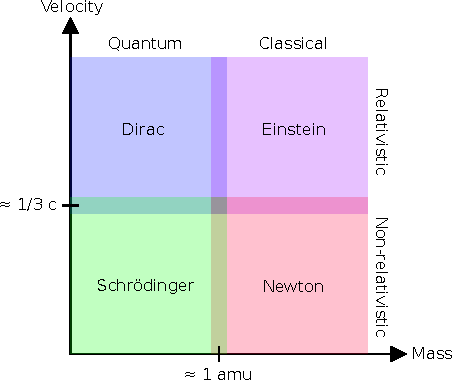
\includegraphics[scale=1.0]{Pics/dyneq}
\caption[Four regimes of dynamical equations]{Dynamical equations can be divided into four regimes, depending on the size and speed of the individual particles. Adapted form \cite{Jen2017}}
\label{fig:REGIMES}
\end{figure}

\section{The Electronic Schrödinger Equation}

\begin{quote}
  "Where did we get that [Schrödinger's equation] from? It's not possible to derive it from anything you know. It came out of the mind of Schrödinger."
  \begin{flushright}
    \small{--- \textit{Richard Feynman, The Feynman Lectures on Physics}}
  \end{flushright}
\end{quote}

If one is interested in describing the electron distribution in detail, the Schrödinger Equation (SEQ) is the best starting point. There is no formal, rigorous proof for the Schrödinger equation, similar to how Newton's second law cannot really be "derived", more than simply "motivated" by observation. 

As successful as the Schrödinger equation is, finding solutions to it is non-trivial. Different approximations may be applied to the SEQ to solve it more easily, without considerable loss of accuracy. 

\subsection{The Time-Independent Schrödinger Equation}

The potential energy operator is the only time-dependent part of the Hamiltonian:
\begin{equation}
\hat{H}(\mbf{r},t) = \hat{T}(\mbf{r}) + \hat{V}(\mbf{r},t)
\end{equation} 
\noindent For systems where the potential is time-independent, e.g. bound systems without external (electromagnetic) perturbation, the Hamiltonian is time-independent as well, which in turn allows to separate space and time variables. It can then be shown that the \emph{time-independent} Schrödinger equation takes the form
\begin{equation}
\hat{H}\Psi(\mbf{r}) = E \Psi(\mbf{r})
\end{equation}
\noindent where $E$ is the total energy of the system, and the eigenvalue of the wave function $\Psi$. The time-dependence is then simply reduced to a phase factor:
\begin{equation}
\Psi(\mbf{r},t) = e^{-iEt} \Psi(\mbf{r})
\end{equation}
\noindent 

\subsection{The Born-Oppenheimer Approximation}

Atomic nuclei are much heavier than electrons ($m_{proton} \approx 1836 m_{electron}$), and move much slower. To a good approximation, the nuclei can be assumed to be stationary from the point of view of electrons. This is known as the \emph{Born-Oppenheimer approximation}. The total Hamiltonian operator can be written in terms of the kinetic and potential operator of the nuclei ($n$) and electrons ($e$) as
\begin{equation}
\hat{H}_{tot} = \hat{T}_n + \hat{T}_e + \hat{V}_{ne} + \hat{V}_{ee} + \hat{V}_{nn}
\label{eq:FULLHAMILTONIAN}
\end{equation}
\noindent In the Born-Oppenheimer approximation, the kinetic energy of the nuclei $T_{nn}$ is neglected, and the nucleus-nucleus potential $V_{nn}$ is taken as a constant, which corresponds to neglecting the coupling between electrons and nuclei. This allows a separation of the electronic and nuclear variables. The remaining terms of Equation \ref{eq:FULLHAMILTONIAN} form the electronic Hamiltonian $\hat{H}_{elec}$. The solutions to the \emph{electronic Schrödinger equation}
\begin{equation}
\hat{H}_{elec} \Psi_{elec}(\mbf{r}_i, \mbf{R}_n ) = E_{elec}(\mbf{R}_n) \Psi_{elec}(\mbf{r}_i, \mbf{R}_n )
\end{equation}
\noindent produce the electronic wave function which depends on the (fixed) \emph{position} $\mbf{R}_n$ of the nuclei and no longer on the \emph{momentum} of the nuclei. The total energy
\begin{equation}
E_{tot}(\mbf{R}_n) = E_{elec}(\mbf{R}_n) + E_{nucl}(\mbf{R}_n)
\end{equation} 
\noindent provides a \emph{potential energy surface} (PES) on which the nuclei move. The PES can then be used to solve the nuclear Schrödinger equation to obtain information on vibrational, rotational and translational properties in the molecular system.

From this point onward, the subscript $elec$ is dropped, and only the electronic Schrödinger Equation is considered.

\section{Solutions to the Electronic Schrödinger Equation}

\subsection{Slater Determinants}

It is beneficial to first consider the wave function of a single electron. In single-atom systems, these functions take the form of "atomic orbitals" (AOs). Correspondingly, "molecular orbitals" (MOs) are defined as the single electron wave functions in a molecular system. These spatial orbital functions form the basis of the full electronic wave function.  

The Hamiltonian in \ref{eq:FULLHAMILTONIAN} only depends on the spatial coordinates. However, to fully describe an electron, spin also needs to be considered. This is done by introducing two orthonormal spin functions $\alpha(\omega)$ and $\beta(\omega)$ corresponding to spin-up ($\uparrow$) and spin-down ($\downarrow$), with the spin-coordinate $\omega$. For one spatial molecular orbital, this gives two possible \emph{spin-orbitals}
\begin{equation}
\phi(\mathbf{x}) = \left\lbrace\begin{matrix}
\varphi(\mathbf{r}) \alpha(\omega) \\
\varphi(\mathbf{r}) \beta(\omega)
\end{matrix} \right.
\end{equation}
\noindent where $\varphi$ are the \emph{spatial orbitals}, and $\mathbf{x}$ are the combined spatial and spin coordinates. The spin orbitals therefore depend on four variables.

To a first approximation, one may consider a molecular system to consist of $N$ \emph{non-interacting}, independent electrons. The Hamiltonian is then written as a sum of one-particle Hamiltonians 
\begin{equation}
\mathbf{H} = \sum_i^N \mathbf{h}_i 
\end{equation}
\noindent Electron correlation may be included in some average way by using \emph{effective} one-electron Hamiltonians, which is the basic working idea of the \emph{Hartree} method. The solution to the SEQ can then be expressed as a product of the one electron wave functions
\begin{equation}
\Psi^{HP}(\mbf{x}_1,\mbf{x}_2,...,\mbf{x}_N) = \phi(\mbf{x}_1) \phi(\mbf{x}_2) ... \phi(\mbf{x}_N)
\end{equation}
\noindent which is also known as \emph{Hartree product}. 

However, the Hartree product does not take into account the \emph{indistinguishability} of electrons. In what is known as the antisymmetry principle, a generalization of the Pauli exclusion principle, the wave function needs to fulfill 
\begin{equation}
\Psi(\mbf{x}_1,\mbf{x}_2) = - \Psi(\mbf{x}_2,\mbf{x}_1) 
\end{equation}
\noindent upon exchange of any two electrons in the system. This is most easily achieved by using \emph{Slater determinants} (SD). For a molecular system consisting of $N$ electrons distributed over $N$ spin orbitals $\phi_i$, the SD takes the form
\begin{equation}
\Psi_{SD}(\mbfx_1, \mbfx_2, \ldots, \mbfx_N) = \frac{1}{\sqrt{N!}}
\begin{vmatrix}
\phi_I(\mbfx_1) & \phi_J(\mbfx_1) & \ldots & \phi_P(\mbfx_1) \\
\phi_I(\mbfx_2) & \phi_J(\mbfx_2) & \ldots & \phi_P(\mbfx_2) \\
\vdots & \vdots & \ddots & \vdots \\
\phi_I(\mbfx_N) & \phi_J(\mbfx_N) & \ldots & \phi_P(\mbfx_N) \\
\end{vmatrix}
\end{equation}
\noindent Or, using the diagonal of the SD as a short-hand notation
\begin{equation}
\Psi_{SD}(\mbfx_1, \mbfx_2, \ldots, \mbfx_N) = \ket{\phi_I(\mbfx_1) , \phi_J(\mbfx_2), \ldots, \phi_P(\mbfx_N)}
\end{equation}

\subsection{The Fock Space}

A more generalized representation of the space of the antisymmetrized electron wave functions can be achieved by introducing the concept of occupation number (ON) vectors in the context of \emph{second quantization} (Appendix \ref{app:SECQUA}). In a system with $M$ possible states (which in the case of molecules correspond to spin molecular orbitals), the ON vectors take the form
\begin{equation}
\ket{\mbf{k}} = \ket{k_1, k_2, \ldots, k_M} = 
\left\lbrace
\begin{matrix}
1 \quad \textit{if $\phi_P$ occupied} \\
0   \quad \textit{if $\phi_P$ occupied}
\end{matrix}
\right.
\label{eq:ONVECTORS}
\end{equation}
\noindent The occupation number is 1 if $\phi_P$ is present in the SD, and 0 if not. Together, all possible ON vectors in Equation \ref{eq:ONVECTORS} form an orthonormal abstract vector space, known as Fock space. The Fock space formed by $N$ electrons distributed over $M$ orbitals is denoted as $F(M,N)$ with total dimension equal to the binomial coefficient $\smash{\binom{M}{N}}$. The sum of the occupation numbers in the ON vectors gives the total number of electrons
\begin{equation}
N = \sum_i^M k_i
\end{equation}
\noindent The special Fock space $F(0,M)$ contains a single vector known as the vacuum state with
\begin{align}
&\ket{vac} = \ket{0_1, 0_2, \ldots, 0_M} \\
&\bra{vac}\ket{vac} = 1
\end{align}
\noindent The ON vectors in $F(M,N)$ can alternatively be expressed in terms of the vacuum state from $F(M,0)$ using creation operators
\begin{equation}
\ket{\mbf{k}} = \left[ \prod_{P=1}^M (a\pdg_P)^{k_P} \right] \ket{vac}
\end{equation}
\noindent In second quantization, the antisymmetry principle of the wave function is guaranteed by the anticommutator relationship of the annihilation and creation operators $a_P$ and $a\pdg_P$ which act on the ON vectors.

\subsection{Exact Solution and Standard Models}

The simplest approach to solving the electronic SEQ is by approximating the exact wave function $\ket{\Psi}$ using a single Slater determinant where the electrons occupy the lowest lying molecular orbitals. The Hartree-Fock method is an example of a \emph{single-determinant method} and finds \emph{the} single best Slater determinant for $\ket{\Psi}$. In Fock space, the best possible determinant is represented by the ON vector where the $N$ lowest lying orbitals are occupied. 

As will be discussed in more detail later, a single-determinant treatment of the electronic wave function is insufficient to fully capture \emph{electron correlation}. The electron correlation energy is formerly defined as the difference between the Hartree-Fock energy and the \emph{exact} energy of $\ket{\Psi}$
\begin{equation}
E_{correlation} = E_{HF} - E_{exact}
\end{equation}
\noindent although the Hartree-Fock wave function does include correlation effects to some degree. In a more general sense, electron correlation is a broad term for any interactions between electrons that make their movement depend on each other, or \emph{correlate} with each other (see Section \ref{sec:CORRELATION}). 

In order to improve on the HF approximation, it is important to add additional Slater determinants. These SDs can be generated from the HF reference wave function by replacing the occupied MOs $\phi_I$ in a reference Slater determinant by one or multiple orbitals $\phi_A$ which were previously unoccupied. This effectively corresponds to exciting one or more electrons from their occupied molecular orbitals $I,J,..$ to unoccupied, or $virtual$ orbitals $A,B,..$. These excited Slater determinants can be classified by the number of electrons they excite and are often referred to as singles, doubles, triples and so on.
\begin{alignat}{2}
\ket{\Phi_0} &= \ket{\HFWFN} \quad & \text{Reference} \\
\ket{\Phi_{I}^{A}} &= a\pdg_A a_I \ket{\HFWFN} \quad & \text{Singles}  \\
\ket{\Phi_{IJ}^{AB}} &= a\pdg_A a_I a\pdg_B a_J \ket{\HFWFN} \quad & \text{Doubles} \\
\ket{\Phi_{IJK}^{ABC}} &= a\pdg_A a_I a\pdg_B a_J a\pdg_C a_K \ket{\HFWFN} \quad & \text{Triples} 
\end{alignat}
\noindent Alternatively, singles states are known as 1-particle-1-hole (1p-1h or simply p-h) states, doubles as 2-particle-2-hole (2p-2h) and so on, due to the excitation operators effectively creating \emph{holes} in the reference determinant and adding \emph{particles} in higher lying orbitals instead. 

The exact solution to the electronic Schrödinger equation is then given by the sum of the Hartree-Fock wave function and all possible ON vectors in $F(M,N)$
\begin{equation}
\ket{\Psi} = c_0 \ket{\HFWFN} + \sum^{\binom{M}{N}-1}_{i=1} c_i  \ket{i} 
\label{eq:EXACTWF}
\end{equation}  
\noindent Equation \ref{eq:EXACTWF} offers a systematic approach to improve on the Hartree Fock method, by increasing (1) the number of Slater determinants and (2) the basis set size $M$, and gives rise to a hierarchy of methods (Figure \ref{fig:STANDARDMODEL}). Correlated electronic structure methods mainly differ by how they determine the expansion coefficients $c$. For all but the smallest systems, the full $F(M,N)$ Fock space cannot be used in calculations due to the total number of ON vectors which increases binomially with $\smash{\binom{M}{N}}$, and hence the number of coefficients to be determined. In practice, the Fock space is \emph{truncated} to some degree.

\begin{figure}
\centering
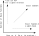
\includegraphics[scale=2.0]{Pics/standardmodel}
\caption[Converging towards the exact wave function]{The wave function converges to the exact solution in the limit of an infinitely large basis set that spans the molecular orbitals, and an infinitely large correlation space spanned by the Slater Determinants.}
\label{fig:STANDARDMODEL}
\end{figure}

\emph{Multi-determinant} methods like configuration interaction (CI) or coupled cluster (CC) use the Hartree Fock wave function as reference from which they generate singles, doubles, triples ... SDs. By truncating at different excitation levels, one gets a hierarchy of CI/CC methods which recover different amounts of correlation energy (e.g. CIS, CISD, CISDT ...). Multi-determinant methods are mainly suited to recover dynamic correlation.

For systems with strong static correlation, additionally, a multi-reference approach is needed. Here, the excited SDs are generated from multiple reference states rather than only from HF. Methods include multi-reference CI (MRCI) and multi-reference CC (MRCC). The reference states are traditionally obtained from multi-configurational self-consistent-field methods (MCSCF) like the complete active space SCF (CASSCF) or restricted active space SCF (RASSCF). MCSCF is a combination of HF and CI, which both optimizes the HF molecular coefficients and the CI expansion coefficients. Multi-reference methods methods mainly recover \emph{static correlation}. 

\subsection{The Variational Method}

The time-independent Schrödinger equation takes the form of an eigenvalue problem
\begin{equation}
\hat{H} \ket{\Psi_i} = E_i \ket{\Psi_i} \qquad i=0,1,2,...\infty
\label{eq:SEQINFTY}
\end{equation}
\noindent where the infinite set of exact solutions $\ket{\Psi_i}$ with eigenvalues $E_i$ forms an orthonormal basis
\begin{equation}
\bra{\Psi_i}\ket{\Psi_j} = \delta_{ij}
\end{equation} 
\noindent A trial wave function can be expanded in the basis of exact solutions with coefficients $c$ as
\begin{equation}
\ket{\tPsi} = \sum_i c_i \ket{\Psi_i}
\label{eq:trialwave}
\end{equation}
\noindent The \emph{variation principle} states that the expectation value of the Hamiltonian of an approximate wave function of the form \ref{eq:trialwave} is an upper bound to the exact ground state energy. This statement can be expressed as
\begin{equation}
\frac{\bra{\tPsi}\hat{H}\ket{\tPsi}}{\vphantom{\widetilde{\Psi}} \bra{\tPsi}\ket{\tPsi}} \geq E_0
\end{equation}
\noindent The equality only holds when $\ket{\tPsi}$ is equal to the exact solution $\ket{\Psi_0}$. One can recast the eigenvalue problem \ref{eq:SEQINFTY} as a variational optimization problem where the energy is a functional of a trial wave function
\begin{equation}
E[\tPsi] = \frac{\bra{\tPsi}\hat{H}\ket{\tPsi}}{\vphantom{\widetilde{\Psi}} \bra{\tPsi}\ket{\tPsi}}
\end{equation}
\noindent The saddle points of the energy functional then correspond to the exact solutions of the Schrödinger equation. The variational approach to the SEQ provides a powerful tool to solve a wide variety of problems in electronic structure theory.

The trial wave function depends on a set of coefficients $c$, and hence the energy functional will also depend on these coefficients. In general, determining the coefficients which minimize the functional is very difficult. However, a more simple approach of the variational method can be obtained by using a linear ansatz where the trial function is expanded in a fixed N-dimensional set of orthonormal basis functions $\ket{\phi}$
\begin{equation}
\ket{\tPsi} = \sum^N_i c_i \ket{\phi_i}
\end{equation}
By using Lagrange's method of undetermined multipliers
\begin{align}
\mathcal{L}(\mbf{c},E) &= \bra{\tPsi}\hat{H}\ket{\tPsi} - E(\bra{\tPsi}\ket{\tPsi} - 1) \\
\frac{\partial \mathcal{L}}{\partial \mathcal{\mbf{c}}} &= 0
\end{align}
\noindent it is possible to show that the variational problem corresponds to solving the eigenvalue problem involving the Hamiltonian matrix $\mbf{H}$:
\begin{equation}
\mbf{H}\mbf{c}_n = E_n \mbf{c_n}
\end{equation}
\noindent Or, in a more general form
\begin{equation}
\mbf{H}\mbf{C} = \mbf{C}\mbf{E}
\end{equation}
\noindent Here, $\mbf{C}$ is a $N$ by $N$ coefficient matrix containing $N$ column coefficient vectors $\mbf{c}_n$ ($n$ = $0...N$) which describe $N$ possible solutions for the trial wave function $\ket{\tPsi}$. $\mbf{E}$ is a diagonal matrix containing the eigenvalues $E_n$. This approach of finding approximate solutions to the eigenvalue problem \ref{eq:SEQINFTY} is known as the \emph{linear variational method}. 

\section{Hartree-Fock}

The Hartree-Fock method is central to electronic structure theory. It is computationally inexpensive, and is still routinely used in qualitative studies of large molecules, even if it does not accurately account for electron correlation. It also serves as the starting point for correlated methods. Only a few computational methods actually bypass the solution to the Hartree-Fock equations, firmly cementing its place in quantum chemistry.

\subsection{The Hartree Fock Equations}

Recall the structure of the electronic Hamiltonian
\begin{equation}
\hat{H} = \hat{T}_e + \hat{V}_{ne} + \hat{V}_{ee} + \hat{V}_{nn}
\end{equation}
\noindent with
\begin{alignat}{2}
\hat{T}_e &= -\sum_i^N \frac{1}{2} \nabla_i^2 & \qquad \textrm{kinetic energy of electrons} \\
\hat{V}_{ne} &= -\sum_a^{N_{nuc}} \sum_i^N \frac{Z_a}{\mid\mbf{R}_a - \mbf{r}_i\mid} & \qquad \textrm{nuclei-electron repulsion} \\
\hat{V}_{ee} &= \frac{1}{2} \sum^N_i \sum^N_{j \neq i} \frac{1}{\mid \mbf{r}_i - \mbf{r}_j\mid} & \qquad \textrm{electron-electron repulsion} \\
\hat{V}_{nn} &= \frac{1}{2}\sum_a^{N_{nuc}} \sum_{b \neq a}^{N_{nuc}} \frac{Z_a Z_b}{\mid \mbf{R}_a - \mbf{R}_b \mid} & \qquad \textrm{nuclei-nuclei repulsion} 
\end{alignat}
\noindent In Hartree-Fock theory, the electrons are treated as independent particles. One can therefore ignore the coupling between electrons in $\hat{V}_{ee}$ and express the Hamiltonian as a sum of an effective one-electron operator $\mbf{f}$, also known as the \emph{Fock} operator, of the form
\begin{align}
\hat{H} &= \sum_i \hat{f}_i =  \sum_i \hat{h}_i + \frac{1}{2} \sum_i \sum_{j \neq i} \hat{g}_{ij} \\
\hat{h}_i &= -\frac{1}{2}\nabla_i^2 - \sum_a^{N_{nuc}} \frac{Z_a}{\mid \mbf{R}_a - \mbf{r}_i |} \\
\hat{g}_{ij} &= \frac{1}{\mid \mbf{r}_i - \mbf{r}_j \mid}
\end{align}
\noindent The one-electron operator $\hat{h}$, also known as the \emph{core} Hamiltonian describes the movement of the electrons in the field of the nuclei. The two-electron operator $\mbf{g}_{ij}$ gives the average potential (or "field") experienced by electron $i$ due to the presence of all the other electrons $j$. For this reason, Hartree-Fock is also known the \emph{mean-field} approximation. In second quantization, the Fock operator takes the form
\begin{equation}
\hat{f} = \sum^{M}_{PQ} h_{PQ} a\pdg_P a_Q + \frac{1}{2} \sum^{M}_{PQRS} g_{PQRS} a\pdg_P a\pdg_R a_S a_Q
\label{eq:FOCK2Q}
\end{equation}
\noindent with the matrix elements of the one and two electron operators given by
\begin{align}
h_{PQ} &= \bra{\phi_P} \mbf{h} \ket{\phi_Q} = \int \phi_P^*(\mbf{x}) h(\mbf{x}) \phi_Q(\mbf{x}) d\mbf{x} \\
g_{PQRS} &= \bra{PQ}\ket{RS} = \int\int \phi_P^*(\mbf{x}_1) \phi^*_R(\mbf{x}_2) g(\mbf{x}_1,\mbf{x}_2) \phi_Q(\mbf{x}_1) \phi_S(\mbf{x}_2) d\mbf{x}_1 d\mbf{x}_2
\end{align} 
\noindent The elements $g_{PQRS}$ are known as the two-electron repulsion integrals. Calculating the expectation values for the Fock operator in \ref{eq:FOCK2Q} using second quantization gives the matrix elements \cite{Hel2000}
\begin{equation}
\begin{split}
f_{PQ} &= \bra{\phi_P} \mbf{f} \ket{\phi_Q} \\
	&= h_{PQ} + \sum_{I}^N \frac{1}{2} (g_{PQII} - g_{PIIQ}) \\
	&= h_{PQ} + \frac{1}{2} (J_{PQ} - K_{PQ})
\end{split}
\end{equation} 
\noindent The symmetric matrix with entries $f_{PQ}$ is also known as the \emph{Fock matrix}. $\mbf{J}$ is the \emph{coulomb matrix} and describes electron correlation due to the coulomb potential (coulomb correlation), and $\mbf{K}$ is the exchange matrix describing the electron correlation which arises due to the Pauli exclusion principle (Fermi correlation). The exchange contributions have no classical counterpart and arise purely from quantum mechanical considerations. 

In the special basis where the Fock matrix is diagonal
\begin{equation}
f_{PQ} = \delta_{PQ} \eps_P 
\end{equation}
\noindent the one-electron eigenfunctions of the Fock operator 
\begin{equation}
\mbf{f} \ket{\phi_P} = \eps_P \ket{\phi_P} 
\label{eq:HFEQ}
\end{equation} 
\noindent are known as the \emph{canonical molecular spin orbitals}, and the eigenvalues are the \emph{molecular orbital energies}. Solving the \emph{canonical Hartree-Fock equation} \ref{eq:HFEQ} gives the MOs which form the basis of the Hartree-Fock wave function. It should be stressed that the total electronic Hartree-Fock energy is not the sum of the individual MO energies, but is given by the expectation value of the Hamiltonian 
\begin{equation}
E_{HF} = \bra{\HFWFN}\hat{H}\ket{\HFWFN} = \sum_{I}^{N} h_{II} + \frac{1}{2} \sum_{I}^{N} \left( J_{II} - K_{II} \right) 
\end{equation}
\noindent which is equivalent to the \emph{trace} of the Hamiltonian matrix $\mbf{H}$. The index $I$ runs over all occupied spin molecular orbitals. For $N$ electrons distributed over $M$ MOs, there are $N$ occupied orbitals with $\eps_I < 0$ and $M-N$ virtual orbitals with $\eps_A > 0$. 

\subsection{The Basis Set Approximation}

Up until this point, the electronic wave function was constructed from Slater determinants of molecular spin orbitals. Virtually all applications use a basis set expansion to express the unknown MOs in terms of known functions, conventionally called \emph{atomic orbitals}. Any type of function can be used, e.g. exponentials, Gaussians, polynomials or plane waves. The molecular orbitals are then expressed as a \emph{linear combination of atomic orbitals} (LCAO)
\begin{equation}
\ket{\phi_i} = \sum_i^{M_{basis}} c_{i\mu} \chi_{\mu} 
\end{equation}
\noindent For molecular systems, there are two types of basis functions that are generally used, namely Slater Type Orbitals (STO) and Gaussian Type Orbitals (GTO):

\begin{align}
\chi_{\zeta, n, l, m}^{STO} (r,\theta ,\phi ) &= N Y_{l,m} (\theta , \phi ) r^{n-1} e^{-\zeta r}
\\
\chi_{\zeta, n, l, m}^{GTO} (r,\theta ,\phi ) &= N Y_{l,m} (\theta , \phi ) r^{2n - 2 - l} e^{-\zeta r^2}
\end{align}

\noindent where N is a normalization constant, $Y_{l,m}$ are spherical harmonics, and $\{n,l,m\}$ are the principal, angular momentum and magnetic quantum number respectively. There are two major differences between STOs and GTOs. At r = 0, STOs have finite slope and GTOs have zero slope. For large r values, GTOs decay much more rapidly than STOs. From an electronic structure point of view, one would prefer to use STOs, as they describe the qualitative features of molecular orbitals better than GTOs. Roughly three time as many GTOs are necessary to obtain the same accuracy as with STOs. Nonetheless, GTOs are preferred, as their drawbacks are outweighed by the relative ease with which their integrals can be evaluated compared to STOs.

\subsection{Working Equations for Restricted and Unrestricted Hartree\-/Fock}

For reasons of efficient implementation, it is useful to separate out different electron spin components. The Fock matrix has four spin blocks: $F_{\alpha\alpha}$, $F_{\alpha\beta}$, $F_{\beta\alpha}$ and $F_{\beta\beta}$. The Fock matrix in the canonical basis is diagonal, and therefore only the diagonal blocks  $F_{\alpha\alpha}$ and $F_{\beta\beta}$ are important. Introducing the notation $\olI$ for MOs with spin $\sigma'$, and $I$ with opposite spin $\sigma$, the matrix elements of a spin block are given by
\begin{equation}
\begin{split}
f_{PQ}^{\sigma} &= h_{PQ}^{\sigma} + \frac{1}{2} \left\lbrace \sum^{N_{\sigma}}_{PQ}\sum^{N_{\sigma}}_{I} \cn{PQ}{II} - \cn{PI}{QI}  - \sum^{N_{\sigma}}_{PQ}\sum^{N_{\sigma'}}_{I} \cn{PQ}{\olJ\olJ} - \cn{P\olJ}{Q\olJ} \right\rbrace \\
&= h_{PQ}^{\sigma} + \sum^{N_{\sigma}}_{PQ} J^{\sigma}_{PQ} - K^{\sigma}_{PQ} + J^{\sigma'}_{PQ} - K^{\sigma'}_{PQ}
\end{split}
\end{equation}
\noindent The opposite spin block $f_{PQ}^{\sigma'}$ is obtained by substituting indices with a bar by indices without a bar and vice-versa. Spin separation yields two coupled sets of equations for alpha and beta MOs
\begin{equation}
\begin{split}
\mbf{f}^{\alpha} \sket{\phi^{\alpha}_I} &= \eps^{\alpha}_I \sket{\phi^{\alpha}_I} \\
\mbf{f}^{\beta} \sket{\phi^{\beta}_I} &= \eps^{\beta}_I \sket{\phi^{\beta}_I} 
\end{split}
\label{eq:UHF}
\end{equation} 
\noindent These are known as the unrestricted Hartree-Fock equations (UHF). For closed-shell molecules with equal number of alpha and beta electrons, the spatial part of the MOs is the same for both spins. The expression for the Fock matrix then further simplifies to 
\begin{equation}
f_{ij} = h_{ij} + 2J_{ij} - K_{ij} 
\end{equation}
\begin{equation}
\mbf{f} \ket{\phi_i} = \eps_i \ket{\phi_i}
\label{eq:RHF}
\end{equation}
\noindent The equations in \ref{eq:RHF} are known as the restricted Hartree-Fock (RHF) equations. 

\noindent Using the linear variatonal method explained in the previous section for the MO trial functions expressed as a linear combination of $N_{bas}$ AO basis functions, the eigenvalue problem for RHF can be recast in matrix form as
\begin{align}
\mbf{F} \mbf{C} &= \mbf{C} \mbf{E} 
\end{align}
\noindent with the MO coefficient matrix $\mbf{C}$ and the Fock matrix $\mbf{F}$ in the AO basis given by
\begin{align}
F_{\mu\nu} &= H^{core}_{\mu\nu} + \sum_{\lambda\sigma}^{N_{basis}} \left[ 2 \cn{\mu\nu}{\sigma\lambda} P_{\lambda\sigma} - \cn{\mu\sigma}{\nu\lambda} P_{\lambda\sigma} \right] \\
&= H^{core}_{\mu\nu} + 2 J_{\mu\nu} - K_{\mu\nu} 
\end{align}
\noindent The symmetric matrix $\mbf{P}$ is the so-called atomic orbital density matrix (DM) of the form
\begin{equation}
P_{\mu\nu} = \sum_i^{N_{occ}} C_{\mu i} C_{\nu i} 
\end{equation}
\noindent A similar expressions is found for UHF
\begin{equation}
\begin{split}
F_{\mu\nu}^{\sigma} &= H^{core}_{\mu\nu} + \sum_{\lambda\sigma}^{N_{basis}} \left( \cn{\mu\nu}{\sigma\lambda} P^{T}_{\lambda\sigma} - \cn{\mu\sigma}{\nu\lambda} P^{\sigma}_{\lambda\sigma} \right) \\
P^T_{\mu\nu} &= P^{\sigma}_{\mu\nu} + P^{\sigma'}_{\mu\nu} 
\end{split}
\end{equation}
\noindent where the AO spin-density matrices $\mbf{P}^{\sigma}$ are defined as the product of the corresponding coefficient matrices with spin $\sigma$.  

\subsection{The Self-Consistent Field Method}

In general, the atomic orbitals are not orthogonal. The overlap matrix $\mbf{S}$ is defined as 
\begin{equation}
S_{\mu\nu} = \int \chi_{\mu}^*(\mbf{r}) \chi_{\nu}^*(\mbf{r}) d\mbf{r}
\end{equation}
\noindent with diagonal entries $S_{\mu\mu} = 1$, and off-diagonal elements $0 < \left\lvert S_{\mu\nu} \right\rvert < 1$. The eigenvalue problem for RHF then takes the more general form
\begin{equation}
\mbf{F} \mbf{C} = \mbf{SC} \mbf{E}
\label{eq:RHALL}
\end{equation}
\noindent The equations in \ref{eq:RHALL} are known as the \emph{Roothan-Hall equations} (RH). In the unrestricted case, they are called the \emph{Pople-Nesbet equations} (PN) which are given by
\begin{align}
\mbf{F}^{\alpha} \mbf{C}^{\alpha} &= \mbf{SC}^{\alpha} \mbf{E}^{\alpha} \\
\mbf{F}^{\beta} \mbf{C}^{\beta} &= \mbf{SC}^{\beta} \mbf{E}^{\beta}
\end{align}  
\noindent The Fock matrix is constructed using the coefficient matrices $\mbf{C}$ to compute the density matrix $\mbf{P}$. This means that the RH (and PN) equations depend on their own solution and must be solved iteratively. Popular choices for iterative schemes include \emph{Newton's} method and the \emph{self-consistent field} (SCF) method, with the latter being the most straight-forward one to implement. 

The SCF procedure is summarized in Algorithm \ref{algo:SCF}. At every iteration, the Fock matrix is diagonalized to obtain a new guess for the density matrix, which is used for constructing the Fock matrix in the next step. These steps are repeated until \emph{self-consistency} is reached. There are different ways to test for convergence, the simplest being the Hartree-Fock energy difference between subsequent iterations. A more rigorous bound is given by the matrix norm of the error vector $\mbf{e}$
\begin{equation}
\mbf{e} = \mbf{FPS} - \mbf{SPF} 
\end{equation}
\noindent At convergence, the density matrix has to commute with the Fock matrix through the overlap matrix. 

\begin{algorithm}
\KwIn{Molecule with nuclear coordinates $\{\mbf{R}_A\}$, atomic numbers $\{Z_A\}$, number of electrons $N$ and basis set $\{\chi_{\mu}\}$}
\KwOut{The matrices $\mbf{F}$, $\mbf{P}$, $\mbf{C}$ and $\mbf{E}$} 
Calculate all one- and two electron integrals
\\
Compute the transformation matrix $\mbf{X}$ from the overlap matrix $\mbf{S}$ with
\begin{equation}
\mbf{X}\pdg \mbf{SX} = \mbf{1} 
\end{equation}
\\
Generate a set of guess orbitals to compute an initial guess density $\mbf{P}$
\\
\While{not converged}{
	Construct the Fock matrix $\mbf{F}$ using the current guess density
	\\
	Orthogonalize the Fock matrix $\mbf{F'} = \mbf{X}\pdg \mbf{FX}$
	\\
	Diagonalize $\mbf{F}'$ to obtain the new orthogonalized MO coefficient matrices $\mbf{C}'$
	\\
	Compute $\mbf{C} = \mbf{X}\mbf{C}$
	\\
	Form the new density $\mbf{P} = \mbf{CC}^T$
	\\
	Check convergence using certain criteria
}
\caption{Hartree-Fock Self-Consistent Field}
\label{algo:SCF}
\end{algorithm}

\subsubsection{SCF Initial Guesses}

The preiteration steps compute the two-electron integrals, the transformation matrix $\mbf{X}$ and a set of guess orbitals. There are different methods for generating a guess. The closer the guess is to the solution, the fewer SCF iterations are needed which saves time. The simplest method consists of using a null matrix for $\mbf{P}$, which corresponds to setting the Fock matrix to the core Hamiltonian $\mbf{H}^{core}$. Diagonalization then gives the guess orbitals. The core Hamiltonian gives a sufficiently close starting guess for small molecules, but is unsuitable for larger molecules. 

The most popular and efficient method at the time of writing is the superposition of atomic densities (SAD) \cite{Van2006}. For each type of atom in the molecule, an atomic HF calculation is carried out which gives the atomic density matrix for this atom type. The molecular guess density matrix is then constructed by setting its diagonal blocks to the atomic densities. The SAD method generates densities that are quite close to the solution. For implementation details, see Appendix \ref{sec:SCFGUESS}.

An alternative starting guess can be obtained by first carrying out a HF calculation with a smaller basis set using the core or SAD guess, and then projecting the density matrix onto the larger basis set (Appendix \ref{sec:SCFGUESS}). This method is especially useful for larger basis sets.  

\subsubsection{SCF convergence}

There is no guarantee that the SCF procedure converges. For small molecules and equilibrium geometries, the unmodified SCF procedure converges quite smoothly. For large, diffuse basis sets or distorted geometries, additional modifications to the algorithms might be necessary:
\begin{enumerate}
\item Direct inversion of the iterative subspace (DIIS): the previous Fock matrices are used for extrapolation to generate a better Fock matrix (section \ref{sec:DIIS})
\item Damping: A damping factor $\omega$ is introduced and the density matrix is replaced by a weighted average $\mbf{P}'_{n+1} = \omega \mbf{D}_n + (1-\omega)\mbf{D}_{n+1}$. Damping is especially useful when the SCF energy oscillates around the equilibrium
\item Level shifting: It has been shown that raising the energy of the virtual orbitals guarantees convergence, at the cost of a decreased convergence rate
\end{enumerate} 

\subsection{Brillouin's Theorem and Orbital Rotations}

The Fock matrix can be divided into four distinct blocks: occupied-occupied, occupied-virtual, virtual-occupied and virtual-virtual. The terms "particle" (p) and "hole" (h) may be used instead of occupied and virtual. In the special case where the orbitals are the canonical MOs, the Fock matrix is diagonal. This is known as the \emph{canonical condition} for the HF wave function. However, diagonality is not necessary for obtaining a valid HF wave function. The general Hartree-Fock equations take the form
\begin{equation}
\hat{f} \phi_P = \sum_{PR} \lambda_{PR} \phi_R
\end{equation}
\noindent Where $\lambda$ are the Lagrange multipliers. For non-canonical MOs, the p-p and h-h are non-diagonal, with elements $\lambda_{IJ}$ and $\lambda_{AB}$ respectively. The off-diagonal elements are computed as
\begin{equation}
f_{IA} = \sbra{\HFWFN}\hat{f}\sket{a\pdg_A a_I \HFWFN} = 0
\end{equation}
\noindent and are zero by virtue of \emph{Brillouin's theorem} for any valid HF wave function. This is also known as the \emph{variational condition}; it is an alternative formulation of the variational principle (see \cite{Hel2000}, section 10.3.5).

The Hartree-Fock energy is therefore stable under unitary rotations
\begin{equation}
\phi_{I'} = \mbf{U} \phi_I \qquad U\pdg U = \mbf{U}
\end{equation}
\noindent The canonical MOs may be rotated to another orbital MO basis with smaller spatial extent, also known as localized molecular orbitals (see Section \ref{sec:ABCLMO}).

\section{Electron Correlation \label{sec:CORRELATION}}

In the Hartree-Fock method, the electron-electron interaction is replaced by an average interaction. For large basis sets, HF is actually able to recover approximately 99\% of the total energy. Unfortunately, the remaining 1\%, the correlation energy, is often important to compute chemical properties with sufficient accuracy.

Electron correlation arises from electrons trying to avoid each other due to coulombic repulsion (coulomb correlation) and the antisymmetry principle (Fermi correlation). This in turn leads to a region of space around each electron where the probability of finding another electron is reduced, typically known as the \emph{coulomb hole} for electrons of opposite spin, and \emph{Fermi hole} for electrons of the same spin. 

Another distinction is often drawn between \emph{dynamic correlation} and \emph{static correlation}, although there exists no formal definition. Dynamic correlation generally describes the correlated movement of electrons due to their "instantaneous mutual repulsion" \cite{Jen2017}. For example, in the ground-state Helium atom, electron correlation is purely dynamical. Static (or non-dynamic) correlation on the other hand arises in the case of near\-/degeneracy, where multiple configurations of similar energy contribute to the ground-state wave function. To show the difference between these two two types of correlation, the dissociation of the H$_2$ molecule is often taken as an illustrative example. At equilibrium distance, correlation is mostly dynamic, and the ground-state can be well described as a singlet state. In the dissociation limit, electrons may be coupled to yield either a singlet \emph{or} a triplet, as the energy difference between those two states vanishes. The correlation in the system is then entirely static. There is no clear-cut line between dynamic and static correlation, but it offers a useful classification for correlation effects.

To fully capture both dynamic and static correlation, it is crucial to add additional Slater determinants as mentioned previously. Methods which generate excited Slater determinants from a single reference SD recover mostly dynamical correlation: electrons are disturbed through their instantaneous repulsion and are excited to higher spin orbitals, hence the need of additional excited-type SDs. Methods generating SDs from multiple references recover mostly static correlation. At the theoretical limit (i.e. the full configuration space), both approaches eventually recover all correlation effects. It is therefore the responsibility of the computational chemist to choose the correct method that best fits the problem at hand.

Any electronic structure method that improves on the HF wave function is usually referred to as a "correlated method". Hartree-Fock, by convention, is an "uncorrelated method". 

For the rest of this report, only single-reference methods are considered.

\section{Configuration Interaction}

\subsection{The CI Matrix}

Configuration interaction (CI) is the simplest and one of the oldest examples of a correlated electronic structure method. The CI wave function takes the general form
\begin{equation}
\ket{\CIWFN} = \sket{\Psi_0} + \sum_{IA} c_{I}^{A} \sket{\Phi_{IA}} + \sum_{\substack{I < J \\ A < B}} c_{IJ}^{AB} \sket{\Phi_{IJ}^{AB}} + \sum_{\substack{I < J < K \\ A < B < C}} c_{IJK}^{ABC} \sket{\Phi_{IJK}^{ABC}} + \dots
\end{equation}
\noindent summing all SDs of all possible types (singles, doubles, triples...). $\Phi_0$ is the reference wave function, here taken as the HF ground state. Whereas the HF wave function was a linear combination of molecular orbitals, the CI wave function is a linear expansion of SDs. Similarly, the CI expansion coefficient matrix $\mbf{C}$ is determined variationally
\begin{equation}
\frac{\partial}{\partial C_i} \frac{\sbra{\CIWFN}\hat{H}\sket{\CIWFN}}{\sbraket{\CIWFN}{\CIWFN}} = 0
\end{equation}
\noindent which, as was shown before, reduces to the eigenvalue problem
\begin{equation}
\mbf{H}\mbf{C} = \mbf{C}\mbf{E}
\end{equation}
\noindent The matrix $\mbf{H}$ is also known as the \emph{CI matrix}. Using the notation $\ket{S}$, $\ket{D}$, $\ket{T}$, ... to denote the set of singles, doubles, triples ... SDs, the CI matrix takes the form
\begin{equation}
\begin{bmatrix}
\bra{\Phi_0}\mbf{H}\ket{\Phi_0} & 0 & \bra{\Phi_0}\mbf{H}\ket{D} & 0 & 0 & \ldots \\
0 & \bra{S}\mbf{H}\ket{S} & \bra{S}\mbf{H}\ket{D} & \bra{S}\mbf{H}\ket{T} & 0 & \ldots \\
\bra{D}\mbf{H}\ket{\Phi_0} & \bra{D}\mbf{H}\ket{S} & \bra{D}\mbf{H}\ket{D} & \bra{D}\mbf{H}\ket{T} & \bra{D}\mbf{H}\ket{Q} & \ldots \\
0 & \bra{T}\mbf{H}\ket{S} & \bra{T}\mbf{H}\ket{D} & \bra{T}\mbf{H}\ket{T} & \bra{T}\mbf{H}\ket{Q} & \ldots \\
0 & 0 & \bra{D}\mbf{H}\ket{Q} & \bra{T}\mbf{H}\ket{Q} & \bra{Q}\mbf{H}\ket{Q} & \ldots \\
\vdots & \vdots & \vdots & \vdots & \vdots & \ddots  
\end{bmatrix}
\end{equation}
\noindent In analogy to the Fock matrix, some blocks in the CI matrix are zero. Brillouin's theorem states that there is no coupling between the ground state and the singlet states. That does not imply that they do not contribute to the CI energy at all. Singles mix \emph{indirectly} via doubles. Moreover, matrix blocks of the Hamiltonian between two SDs which differ by more than two spin orbitals are also zero. Triples mix with doubles and singles, but not with the ground state.

A more compact representation of the CI matrix is obtained by taking linear combinations of SDs in the same excitation manifold, known as configuration state functions (CSF) or spin-adapted configurations (SAC). The CSFs form a basis smaller than that composed of all individual SDs which leads to computational savings. However, CSFs were primarly introduced to preserve the spin symmetry of the ground state, or in other words, CSFs are eigenfunctions of the $\mbf{S}^2$ operator. If the HF ground state is a singlet, a non-spin-symmetric CI basis may lead to the CI wave function being a mixture of singlet and triplet determinants. 

\subsection{Truncated CI}

Full CI, i.e. including all excitation manifolds, is only computationally feasible for the smallest molecules, due to the binomial increase in the number of SDs as a function of system and basis set size. For this reason, the CI wave function is often truncated at a given excitation level. Including only singles gives configuration interaction with singles (CIS), including singles and doubles yields configuration interaction with singles and doubles (CISD), etc. Higher order methods recover a larger fraction of the correlation energy, but come at a higher computational cost.

It should be noted that the energy of the CIS wave function is equal to the HF energy due to Brillouin's theorem, and hence does not contribute to the correlation energy of the ground state.  

\subsection{Solving the CI Eigenvalue Problem}

Even at relatively low truncation levels, the number of matrix elements have a quite steep polynomial scaling with $\ccpx{6}$ for CISD and $\ccpx{8}$ for CISDT. In most cases however, only the few lowest eigenvalues are needed. Davidson's method of matrix diagonalization (section \ref{sec:DAV}) was specifically developed to tackle this problem. Rather than storing the whole matrix, only matrix-vector products need to be computed
\begin{equation}
\mbf{r} = \mbf{M}_{CI} \mbf{u}
\end{equation}
\noindent Closed expressions can be derived and the full matrix is not explicitly needed, but generated on-the-fly. 

\subsection{Size Consistency and Size Extensivity}

Over the years, single-reference truncated CI methods have fallen out of favor for more sophisticated methods, due to CI not being size-consistent and size-extensive. \emph{Size-consistency} refers to the idea that the energy of two non-interacting systems $A$ and $B$ should be equal to the sum of their individual energies obtained from two different calculations:
\begin{equation}
E(A+B) = E(A) + E(B)
\end{equation}
\noindent \emph{Size-extensivity} is a closely-related criterion that states that the energy should be a linear function of the number of electrons , i.e. the energies of small and large molecules have similar errors, which is important for comparing properties \cite{You2004}. As the system size increases, truncated CI recovers less and less of the total correlation energy.

\section{Coupled Cluster}

The coupled-cluster (CC) approximation offers a more sophisticated picture of electron correlation than CI, and has become one of the most successful and accurate \emph{ab initio} correlated methods. It is both size-consistent and size-extensive.

\subsection{Pair Clusters}

Consider a system composed of two electrons, occupying the orbitals $I$ and $J$ in the independent particle model. Correlation manifests itself by the electrons' instantaneous repulsion and excitation into higher lying orbitals. Mathematically, this may be expressed as \cite{Hel2000}
\begin{equation}
a\pdg_I a\pdg_J + \sum_{A > B} t_{IJ}^{AB} a\pdg_A a\pdg_B = \left( 1 + t_{IJ}^{AB} \hat{\tau}_{IJ}^{AB} \right) a\pdg_I  a\pdg_J 
\label{eq:epair}
\end{equation}
\noindent where $\mbf{t}$ are the associated cluster coefficients, also known as \emph{amplitudes}. By virtue of Brillouin's theorem, single excitations are not considered. Equation \ref{eq:epair} is known as the \emph{electron pair}, \emph{two-electron cluster} or \emph{pair-cluster} approximation. 

In a first approximation, electron pairs may be treated independently in a molecular system, in what is known as the independent electron pair approximation (IEPA). The total correlation energy is then simply given as the sum of the individual \emph{pair correlation energies}
\begin{align}
E_{corr}^{IEPA} &= \sum_{I < J} e_{IJ}  \\
\ket{\textrm{IEPA}} &= \sum_{I < J, A < B} \left(1 + t_{IJ}^{AB}\hat{\tau}_{IJ}^{AB} \right) \ket{\HFWFN} 
\end{align}
\noindent A more complete picture of electron correlation is given by additionally letting electron clusters interact with each other by using the parametrization
\begin{equation}
\ket{\textrm{CCD}} = \left( \prod_{A > B,I > J} 1 + t_{IJ}^{AB}\hat{\tau}_{IJ}^{AB} \right) \ket{\HFWFN}
\end{equation}
\noindent The resulting wave function corresponds to the coupled cluster approximation including only doubles (CCD). As opposed to CID, CCD additionally includes \emph{products} of doubles cluster operators ($\tau_{IJ}^{AB} \tau_{KL}^{CD}$, or $\tau_{IJ}^{AB} \tau_{KL}^{CD} \tau_{MN}^{EF}$), in other words, doubles excitations are included up to infinite order. It is this property that makes CC size-extensive.

% ref R J Bartlett J Phys Chem 93 (1996) 216

\subsection{Coupled Cluster Ansatz}

The CCD model can be generalized to let clusters of three and more electrons interact with each other, and electrons interact within these clusters. The general CC ansatz reads
\begin{equation}
\ket{\CCWFN} = \left( \prod_{\mu} 1 + t_{\mu}\hat{\tau}_{\mu} \right) \ket{\HFWFN} = exp(t_{\mu}\hat{\tau}_{\mu}) \ket{\HFWFN} = exp(\hat{T}_{\mu}) \ket{\HFWFN}
\label{eq:CCANSATZ}
\end{equation}
\noindent where $\hat{T}_{\mu}$ is the \emph{cluster operator}, and $\mu$ are the excitation manifolds. The cluster operator may be partitioned into classes comprising all singles, doubles, ... excitations:
\begin{equation}
\hat{T} = \hat{T}_1 + \hat{T}_2 + ... + \hat{T}_N
\end{equation}
\noindent Truncating the cluster operator to include only excitations up to a certain degree yields a hierarchy of CC method named CCS, CCSD, CCSDT etc. Again, including higher orders implies a higher computational effort. The exponential in Equation \ref{eq:CCANSATZ} for different truncation levels is approximated as
\begin{align}
exp(\hat{T}) &= \hat{T}_1 \\
exp(\hat{T}_1 + \hat{T}_2) &= \hat{T}_2 + \frac{1}{2} \hat{T}_1^2 \\
exp(\hat{T}_1 + \hat{T}_2 + \hat{T}_3) &= \hat{T}_3 + \hat{T}_1 \hat{T}_2 + \frac{1}{6} \hat{T}_1^3 \\
\ldots \nonumber
\end{align}
\noindent Triplet configurations for example are generated by three mechanisms. $\hat{T}_3$ is known as a \emph{connected} term, and the other terms which are products of lower order operators are known as \emph{disconnected} terms. 

\subsection{The Coupled Cluster Equations} 

The cluster amplitudes are unknown and need to be solved for. Equations for the amplitudes can be obtained by projecting the Schrödinger equation with the CC ansatz \ref{eq:CCANSATZ} onto the excitation manifolds. Using the so-called \emph{similarity-transformed} Hamiltonian
\begin{equation}
\hat{\bar{H}} = exp(-\hat{T}) \hat{H} exp(\hat{T})
\end{equation} 
\noindent gives the set of non-linear equations
\begin{align}
\begin{split}
\bra{\mu_1}\hat{\bar{H}}\ket{\HFWFN} &= 0 \\
\bra{\mu_2}\hat{\bar{H}}\ket{\HFWFN} &= 0 \\
\bra{\mu_3}\hat{\bar{H}}\ket{\HFWFN} &= 0 \\
\vdots & 
\end{split} 
\label{eq:CCEQ}
\end{align}
\noindent where $\mu_n$ is the $n$th order excitation manifold (singles, doubles ....). The exact expressions of the CC amplitude equations at different truncation levels may be evaluated using the 
Baker–Campbell–Hausdorff (BCH) formula, but will not be discussed in detail here. As an example of the exact form of the working equations, consider the CCSD model truncated at doubles excitation. Equation \ref{eq:CCEQ} then reduces to
\begin{align}
\sbra{\mu_1} \hat{\bar{H}} + \left[\hat{\bar{H}},\hat{T}_2\right] \sket{\HFWFN} = 0 
\label{eq:CCSDEQSINGLES}
\\
\sbra{\mu_2} \hat{\bar{H}} + \left[\hat{\bar{H}},\hat{T}_2\right] + \frac{1}{2} \left[ \left[ \hat{\bar{H}},\hat{T}_2\right],\hat{T}_2\right] \sket{\HFWFN} = 0
\label{eq:CCSDEQDOUBLES}
\end{align}
The system of equations \ref{eq:CCEQ} depends on its own solution, and therefore needs to be solved iteratively. They are most commonly solved using a modified Newton method with DIIS acceleration. 

\section{Perturbation Theory}

Coupled cluster and configuration interaction offer a systematic way to move towards the exact solution to the Schrödinger equation by means of adding more Slater determinants. However, the calculation of the  CC and CI wave functions is very expensive, and it may be profitable to look at alternative schemes. \emph{Perturbation theory} (PT) is a different approach to systematically close in on the exact wave function. It is based on the idea that the exact solution differs only slightly from a previously solved problem for a simpler, related system.

\subsection{Rayleigh-Schrödinger Perturbation Theory}

Perturbation theory is used in a wide range of fields and disciplines in natural sciences and mathematics. In the context of molecular electronic structure theory, the most widely used form of PT is Rayleigh-Schrödinger perturbation theory (RSPT). In RSPT, the Hamiltonian is partitioned according to
\begin{equation}
\hat{H} = \hat{H}_0 + \hat{U}
\end{equation}
\noindent where $\hat{H}_0$ is some reference zero-order Hamiltonian with known eigenfunctions $\ket{\Psi^{0}_i}$ and eigenvalues $E_i^{0}$. $\hat{U}$ is a small perturbation to the system. The exact wave function and energies may be expanded in orders of the perturbation
\begin{align}
\ket{\Phi_i} &= \sum_{k=0}^{\infty} \sket{\Psi_i^{(k)}} \label{eq:RSPTWF} \\
E_i &= \sum_{k=0}^{\infty} E_i^{(k)} \label{eq:RSPTEN}
\end{align} 
\noindent The task at hand is to derive closed expressions for higher order terms of order $n$ using terms of order $n-1$ and lower. Substituting the expressions \ref{eq:RSPTWF} and \ref{eq:RSPTEN} into the Schrödinger equation gives
\begin{equation}
\left(\hat{H}_0 + \hat{U}\right) \sum_{k=0}^{\infty} \sket{\Psi_i^{(k)}} = \left( \sum_{k=0}^{\infty} E_i^{(k)} \right) \left( \sum_{k=0}^{\infty} \sket{\Psi_i^{(k)}} \right)
\label{eq:RSPTSEQ}
\end{equation}
\noindent Collecting terms of order $n$, the above expression may be rewritten as a system of equations involving the residual of the Hamiltonian:
\begin{equation}
(\hat{H}_0 - E_i^{(0)}) \sket{\Psi_i^{(n)}} = -\hat{U} \sket{\Psi_i^{(n-1)}} + \sum_{k=1}^{n} E_i^{(k)} \sket{\Psi_i^{(n-k)}}
\label{eq:RSPTSEQ2}
\end{equation}
\noindent Or alternatively, when multiplied with the inverse of the Hamiltonian residual:
\begin{equation}
 \sket{\Psi_i^{(n)}} = - (\hat{H}_0 - E_i^{(0)})^{-1} \left( \hat{U} \sket{\Psi_i^{(n-1)}} + \sum_{k=1}^{n} E_i^{(k)} \sket{\Psi_i^{(n-k)}} \right)
\label{eq:RSPTSWF}
\end{equation}
\noindent Furthermore, to obtain simpler expressions for $E_i^{(k)}$, the normalization is chosen such that $\sbraket{\Psi_i^{(0)}}{\Phi_i}=1$, also known as intermediate normalization. From this it follows that the approximate wave functions are orthogonal to the reference states
\begin{equation}
\sbraket{\Psi_i^{(0)}}{\Psi_i^{(n)}} = 0 \qquad n = 1,2,3,\ldots
\label{eq:RSPTORTHO}
\end{equation}
\noindent Left-projection of $\sbra{\Psi_i^{(0)}}$ onto the system of equations in \ref{eq:RSPTSEQ2} and using the orthogonality condition \ref{eq:RSPTORTHO} yields the master equations for the RSPT energies
\begin{equation}
E_i^{(n)} = \sbra{\Psi_i^{(0)}} \hat{U} \sket{\Psi_i^{(n-1)}} \qquad n > 0
\label{eq:RSPTENEQ}
\end{equation}

\noindent The approximate energy expressions can be solved for without the need of iterative procedures, and closed expressions may be derived for a given reference. One way of solving \ref{eq:RSPTENEQ} is to expand the first-order wave function in terms of the the eigenfunctions of $\hat{H}_0$:
\begin{equation}
\sket{\Psi_i^{(1)}} = \sum_n c^{(1)}_n \sket{\Psi_i^{(0)}}
\end{equation}
\noindent Multiplying from the left by $\sbra{\Psi_n^{(0)}}$, the expansion coefficients can be obtained with
\begin{equation}
\sbraket{\Psi_n^{(0)}}{\Psi_i^{(1)}} = c_n^{(1)}
\end{equation}
From the expression of the first order wave function in \ref{eq:RSPTWF}
\begin{equation}
\sket{\Psi_i^{(1)}} = - (\hat{H}_0 - E_i^{(0)})^{-1} (\hat{U} + E_i^{(1)}) \sket{\Psi_i^{(1)}} 
\end{equation}
\noindent it follows that the first order expansion coefficients are given by
\begin{equation}
c_n^{(1)} = \frac{\sbra{\Psi_n^{(0)}} \hat{U} \sket{\Psi_0^{(0)}}}{E_i^{(0)} - E_n^{(0)}} 
\end{equation}
\noindent Higher order energy expressions can then be "build up" step by step from lower order approximations following the normalization and orthogonality conditions. The first few closed-form RSPT energy expressions are given by
\begin{align}
E_0^{(1)} &= \sbra{\Psi_0^{(0)}} \hat{U} \sket{\Psi_0^{(0)}} \\
E_0^{(2)} &= \sum_n \frac{
	\left\lvert \sbra{\Psi_0^{(0)}} \hat{U}\sket{\Psi_n^{(0)}} \right\rvert^2
}{
	E_0^{(0)} - E_n^{(0)}
} \\
\begin{split}
E_0^{(3)} &= \sum_{nm} \frac{
	\sbra{\Psi_0^{(0)}}\hat{U}\sket{\Psi_n^{(0)})}
	\sbra{\Psi_n^{(0)}}\hat{U}\sket{\Psi_m^{(0)}}
	\sbra{\Psi_m^{(0)}}\hat{U}\sket{\Psi_0^{(0)}}
}{
	(E_0^{(0)} - E_n^{(0)})(E_0^{(0)} - E_m^{(0)})
} \\
&- E_0^{(1)} \sum_n \frac{
	\left\lvert \sbra{\Psi_0^{(0)}} \hat{U}\sket{\Psi_n^{(0)}} \right\rvert^2
}{
	(E_0^{(0)} - E_n^{(0)})^2
} 
\end{split} \\ \nonumber
\ldots
\end{align}

\subsection{M{\o}ller-Plesset Perturbation Theory}

The success of RSPT is closely related to the choice of the zero-order Hamiltonian. The most popular variant of RSPT is M{\o}ller-Plesset perturbation theory (MPPT), where $\hat{H_0}$ is taken as the Fock operator from HF theory
\begin{equation}
\hat{H}_0 = \hat{f} = \sum_P \eps_P a\pdg_P a_P
\end{equation}
\noindent The zero-order wave function $\sket{\Psi_0^{(0)}}$ corresponds to the Hartree Fock wave function $\sket{\HFWFN}$. The perturbation operator takes the form
\begin{equation}
\hat{U} = \hat{H} - \hat{f} = \sum_{PQRS} \hat{g}_{PQRS} a\pdg_P a\pdg_R a_S a_Q - \hat{V}^{HF} 
\end{equation}
\noindent where $V^{HF}$ is the Hartree-Fock potential. The zero-order component of the ground state energy is simply given as the sum of the orbital energies
\begin{equation}
E_0^{(0)} = \sum_I \eps_I
\end{equation}
\noindent The first order energy is
\begin{equation}
\begin{split}
E_0^{(1)} &= \sbra{\Psi_0^{(0)}} \hat{U} \sket{\Psi_0^{(0)}} \\
&= \sbra{\HFWFN}\hat{U}\sket{\HFWFN} \\
&= -\frac{1}{2} \sum_{IJ} ( \sbraket{IJ}{IJ} - \sbraket{IJ}{JI} ) \\
&= -\frac{1}{2} \sum_{IJ} \sbra{IJ}\sket{IJ} 
\end{split}
\end{equation}
\noindent where $\sbra{IJ}\sket{IJ}$ are the antisymmetrized two-electron integrals in the MO basis. The energy sum $E_0^{(0)} + E_0^{(1)}$ corresponds to the Hartree-Fock energy. Therefore, the first correction to the Hartree-Fock energy occurs at the second order of MPPT. Using the notation MP$n$ to refer to MPPT including perturbations up to the $n$th order, the second order energy reads
\begin{equation}
\begin{split}
E_0^{(2)} = E_{MP2} = \frac{1}{4} \sum_{IJAB} \frac{\abs{ \sbra{IJ}\sket{AB}}^2}{\eps_I + \eps_J - \eps_A - \eps_B}
\end{split} 
\label{eq:UMP2}
\end{equation}
\noindent For a closed-shell molecule, the restricted MP2 energy can be obtained by spin-separation similarly to how it was done in Section 1.4.3 for Hartree-Fock:
\begin{equation}
\begin{split}
E_{RMP2} &= \sum_{ijab} \frac{\cn{ia}{jb}\left[2\cn{ia}{jb} - \cn{ib}{ja} \right]}{\eps_i + \eps_j - \eps_a - \eps_b} \\
&= \sum_{ijab} t_{iajb} \left[\cn{ia}{jb} - \cn{ib}{ja} \right]
\end{split}
\label{eq:RMP2}
\end{equation}
\noindent where $\mbf{t}$ are the MP2 amplitudes. Furthermore, the MP2 energy may be split into individual electron pair contributions, analogous to CC:
\begin{equation}
E_{MP2} = \sum_{ij} e_{ij}
\end{equation}
\noindent The energy expressions for MP3 and beyond will not be discussed here.

\subsection{Convergence Behavior of the MP$n$ series}

MP2 is a computationally cheap correlated method that includes 80\% to 90\% of electron correlation method, scaling with $\ccpx{5}$ as a function of the system size $N$. Higher order variants like MP3 or MP4 are considerably less popular. 

Ideally, the MP$n$ energy should converge monotonically towards the limit with increasing order of perturbation. However, such a behavior is not guaranteed. Contrary to the CI energy, which is determined variationally and therefore has a lower bound, the same is not true for MPPT and the MP$n$ series may become divergent or oscillating for larger basis sets, especially if diffuse functions are used. MP2 improves on the HF wave function, but slightly overestimates correlation energy. MP3 underestimates electron correlation, and properties computed at this level are often inferior to those computed at second order. MP4 again overestimates correlation effects, but is better than MP2.

Due to the erratic convergence behavior of MPPT, higher order variations like MP3 or MP4 have fallen somewhat out of favor in recent years. Moreover, the requirement of the single-determinant HF wave function being a suitable starting guess makes MPPT ill-suited to describe static correlation effects.  

\subsection{M{\o}ller-Plesset Perturbation Theory with Spin-Component-Scaling \label{sec:SCSMP2}}

With the rise of density functional theory (DFT), even the computationally inexpensive MP2 method fell out of use in favor of DFT which often shows better performance and accuracy for the same molecular systems.

In the early 2000s, MPPT again gained more popularity with the introduction of \emph{spin-component scaling} (SCS) by Grimme et al. \cite{Gri2003,Gri2012} which greatly improves on the accuracy of MP2.

Consider again the MP2 energy in the unrestricted case in Equation \ref{eq:RMP2}. The energy contributions can be split into same-spin (SS) and opposite spin (OS) components:
\begin{align}
E_{MP2-SS} &= \sum_{IJ} e_{IJ} + e_{\olI\olJ} \\
E_{MP2-OS} &= \sum_{IJ} e_{I\olJ} 
\end{align}
\noindent with
\begin{align}
e_{IJ} &= \sum_{AB} t_{IAJB} (\cn{IA}{JB} - \cn{IB}{JA}) \\
e_{\olI\olJ} &= \sum_{AB} t_{\olI\olA\olJ\olB} (\cn{\olI\olA}{\olJ\olB} - \cn{\olI\olB}{\olJ\olA}) \\
e_{I\olJ} &= \sum_{AB} t_{IA\olJ\olB} \cn{IA}{\olJ\olB}  
\end{align}
The correlation effects in SS and OS are of different nature as discussed in Section \ref{sec:CORRELATION}. Hartree-Fock accounts for Fermi correlation by the antisymmetry principle but does not fully account for Coulomb correlation. MP2 cannot fully rectify this deficiency in the starting guess. SCS-MP2 accounts for this behavior by scaling down the SS components and scaling up the OS components
\begin{equation}
E_{SCS-MP2} = c_{os} E_{OS-MP2} + c_{ss} E_{SS-MP2}
\end{equation}
\noindent where the scaling factors are determined empirically by fitting to a data set, with $c_{ss}$ = 6/5 and $c_{os}$ = 1/3. In later iterations of SCS-MP2, the two parameters were unified by introducing the relationship
\begin{equation}
c_{ss} = 4 - 3c_{os}
\end{equation}
\noindent whit $c_{ss}$ and $c_{os}$ set to 0.4 and 1.2 respectively.

SCS-MP2 gives considerable improvements to reaction energies \cite{Gri2003}, barrier heights \cite{Gou2004,Bul2004}, geometries and vibrational frequencies \cite{Ger2004}, comparable to QCISD(T) with errors on the order of 1.7 kcal/mol. Strictly speaking, SCS-MP2 is no longer an \emph{ab initio} method, but \emph{semi-empirical}. SCS was initially an \emph{ad-hoc} improvement to the description of the wave function, but it is possible to justify its position in the theoretical framework of MPPT \cite{Sza2006,Fin2010}. 

Over the years, many different variations of SCS-MP2 have been proposed \cite{Jun2004,Loc2005,Dis2007,Hil2007}. One variation is the so-called spin-opposite scaled (SOS) MP2 method \cite{Jun2004}, where the SS components are simply ignored:
\begin{equation}
E_{SOS-MP2} = c_{os} E_{OS-MP2}
\end{equation}
\noindent with $c_{os}$ set to 1.3 instead of 1.2 as in SCS-MP2. The method can be justified by observing that the SS components already do not contribute a lot to the SCS-MP2 energy. SOS-MP2 has comparable or slightly worse accuracy than SCS-MP2. The major advantage which makes SOS-MP2 one of the more attractive spin-component scaling variants is the reduced scaling $\ccpx{4}$ compared to $\ccpx{5}$ for (SCS)-MP2 when the density-fitting approximation is used.
% within that: 16, 19, 20, 23, 24, 28, 25 40, 41, 42

\subsection{Hybrid Coupled Cluster Methods}

Perturbational approaches may also be used to obtain approximate hybrid coupled cluster methods. 

Consider again the CCSD equations for the coupled cluster singles \ref{eq:CCSDEQSINGLES} and doubles amplitudes \ref{eq:CCSDEQDOUBLES}. Introducing the same partitioning of the Hamiltonian as in MP2 with
\begin{equation}
\hat{H} = \hat{F} + \hat{U}
\end{equation}
\noindent where $\hat{U}$ is also known as the \emph{fluctuation potential}, the coupled cluster singles doubles method by Christiansen et al. \cite{Chr1995} approximates the doubles amplitudes to first order only. The doubles equation \ref{eq:CCSDEQDOUBLES} thus becomes
\begin{equation}
\sbra{\mu_2} \left[ \hat{F}, \hat{T}_2\right] + \hat{\ovl{H}} \sket{\HFWFN} = 0
\label{eq:CC2EQDOUBLES}
\end{equation}
\noindent Equations \ref{eq:CCSDEQSINGLES} and \ref{eq:CC2EQDOUBLES} define the so-called \emph{CC2} model. The doubles equations give an MP2-like closed expressions, and only the singles amplitudes need to be determined variationally.

The CC2 energy has a similar accuracy and computational effort to MP2. Spin-component scaling has been generalized to CC2 as well \cite{Hel2008,Win2011}, with similar improvements to its accuracy \cite{Taj2019}. 

Higher order CC methods like CCSDT can be approximated in a similar way to obtain the approximate CC3 method \cite{Koc1997}, where triples contributions are approximated to second order. A related method is the coupled cluster singles doubles with perturbative non-iterative triples method \cite{Rag1989}, abbreviated as CCSD(T), where triples contributions to the energy are added to the CCSD ground state energy. CCSD(T) and CC3 have comparable accuracy and cost. 

% 1 DOI: 10.1039/b803727b Hel2008
% 2 DOI: 10.1063/1.3584177 Win2011
% 3 https://doi.org/10.1021/acs.jctc.9b00676 Taj2019 
% 4 https://doi.org/10.1063/1.473322 Koc1997
% 5 K. Raghavachari, G. W. Trucks, J. A. Pople, and M. Head-Gordon, Chem. Phys. Lett. 157, 479 (1989) Rag1989

\section{Performance of Correlated Methods}

The previous sections give insight into the most popular, single-determinant, correlated electronic structure methods. The methods vary widely in accuracy, computational cost and convergence behavior. 

Table \ref{tab:SCALINGS} gives the formal computational scaling for some of the methods. The notation $\mathcal{O}()$, also known as \emph{Big O notation}, is the standard way of indicating the limiting behavior of algorithms for increasing input size. $N$ is used as a measure of the molecular system size (e.g. number of atoms or basis functions). \emph{Formal} scaling means that factors like sparsity or locality are not considered.

\begin{table}
\centering
\begin{tabular}{lllll} 
\hline 
Scaling & Non-correlated & CI methods & CC methods & MP methods \\ \hline
$\ccpx{4}$ & HF &  &  &  \\
$\ccpx{5}$ & & CIS & CC2, SCS-CC2 & MP2, SCS-MP2 \\
$\ccpx{6}$ & & CISD & CCSD & MP3 \\
$\ccpx{7}$ & & & CC3, CCSD(T) & MP4 \\
$\ccpx{8}$ & & CISDT & MP5 & CCSDT \\
\hline 
\end{tabular}
\caption{Formal scaling of popular electronic structure methods}
\label{tab:SCALINGS}
\end{table}

At the time of writing, on current work stations, $\ccpx{5}$ methods are limited to system sizes of around 50 to 100 atoms, and $\ccpx{6}$ to sizes of several tens of atoms. Models with $\ccpx{7}$ scaling and beyond are not used routinely. 

In terms accuracy, the current trend is often observed \cite{Jen2017}:

\begin{equation}
HF << MP2 \approx CC2 < CCSD < MP4 < CCSD(T) 
\end{equation}




\chapter{Local Correlation Methods (I): Tools and Concepts \label{cha:LOCAL0}}

While computational chemistry has emerged as a reliable experimental tool, the inherent steep scaling of its most accurate methods like coupled cluster or perturbation theory often imposes strict limits on the maximum molecular system size that can be treated. Even the Hartree-Fock method formerly scales with O(N$^4$), and becomes prohibitively expensive for larger molecules if no further approximations are introduced. For post-Hartree-Fock methods, the major bottle necks are the transformation of the 2-electron repulsion integrals from the atomic orbital into the molecular orbital basis, and evaluation of the working equations using these integrals. The $OVOV$-type MO integrals, as they appear in coupled cluster and M{\o}ller-Plesset perturbation theory, are given by
\begin{equation}
\cn{ia}{jb} = \sum^{vir}_b C_{\sigma b} \sum^{vir}_a C_{\nu a} \sum^{occ}_j C_{\lambda j} \sum^{occ}_i C_{\mu i} \cn{\mu\nu}{\lambda\sigma}
\end{equation}
The AO-MO transformation step scales quartically with system size. Over the years, several different strategies have been proposed to speed up this step. Rank-reduction approaches like density fitting or the Cholesky decomposition, split the 4-index integral tensor into a product of two 3-index tensors, which reduces the memory footprint and the \emph{prefactor} of the transformation. Methods that exploit the nearsightedness of the electrons use a different molecular orbital representations, such as local molecular orbitals or natural orbitals, to obtain a more compact representation of the virtual MO space, and consequently reduce the \emph{scaling}. The AO-MO transformation may also be completely skipped by reformulating the working equations in an atomic orbital basis and using sparsity to speed up the calculations.

This chapter introduces the most important tools used in local correlation methods which will be discussed in the next chapter.

\section{Sparsity in Electronic Structure Theory}

Sparsity is a core concept in electronic structure theory. Many of the most commonly encountered matrices and tensors exhibit some form of sparsity, for example, the 2-electron repulsion integrals in the AO basis. This section analyses in detail the different possible types of sparsity.

\FloatBarrier

\subsection{Element-Wise Sparsity of Electron Integrals}

Molecular electron integral evaluation can become prohibitively expensive for large systems, especially the four-dimensional electron-repulsion integral (ERI) tensor which formerly scales as $\ccpx{4}$. It is therefore imperative to exploit the exponential decay of the GTO basis.

Consider a model system consisting of $n$ hydrogen atoms arranged in a line, with a distance of 1 $a_0$ between one another, and a primitive 1s Gaussian function attached to each atom. Figure \ref{fig:HCHAIN_ERINZE} shows the scaling behavior of the overlap and electron repulsion integrals for this toy system. A blue line is used to show the number of total elements, while the green line represents the number of significant integrals with an absolute value below 1e-10. From observing both graphs, it becomes apparent that for increasing number of atoms, many of the electron integrals can be ignored. Therefore, one only needs to store integrals above a certain threshold. This is also known as \emph{element-wise sparsity}.

\begin{figure}[h]
\centering
\begin{subfigure}{0.45\linewidth}
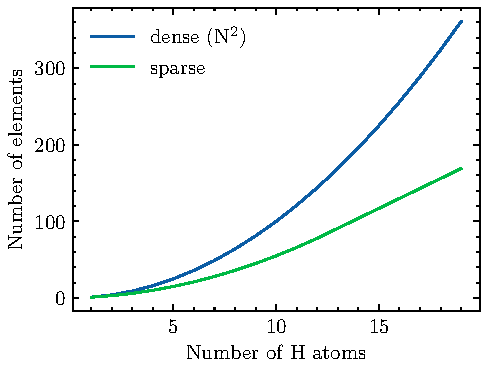
\includegraphics[scale=0.8]{overlap_nze}
\caption{}
\end{subfigure}
\begin{subfigure}{0.45\linewidth}
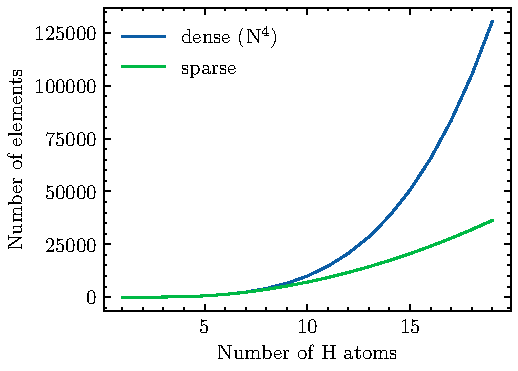
\includegraphics[scale=0.8]{eri_nze}
\caption{}
\end{subfigure}%
\caption{(a) Number of significant entries (green line) in the overlap matrix for a hydrogen atom chain, with a threshold of 1e-10. The blue line shows the total number of elements for the dense matrix, which scale as $N^2$. (b) Number of significant entries (green line) in the electron repulsion integral tensor for a hydrogen atom chain, with a threshold of 1e-10. The blue line shows the total number of elements for the dense tensor, which scale as $N^4$.}
\label{fig:HCHAIN_ERINZE}
\end{figure}

\begin{figure}
\centering
\begin{subfigure}{0.45\linewidth}
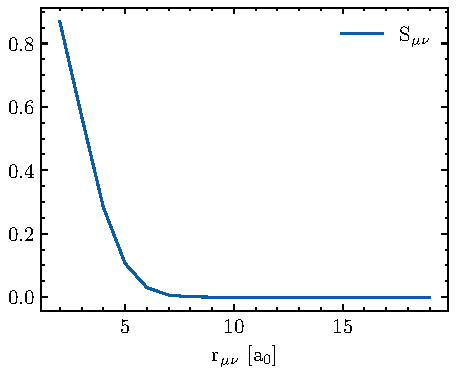
\includegraphics[scale=0.8]{overlap_decay}
\caption{}
\end{subfigure}
\begin{subfigure}{0.45\linewidth}
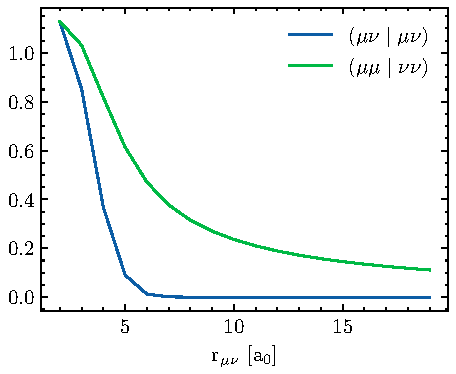
\includegraphics[scale=0.8]{eri_decay}
\caption{}
\end{subfigure}%
\caption{(a) Magnitude of the overlap integral between two Gaussian 1s orbitals as a function of distance $r$ (exponential decay). (b) Magnitude of the electron repulsion integral between two Gaussian 1s orbitals as a function of $r$. The short range interaction $\cn{\mu\nu}{\mu\nu}$ decays at a  much faster rate with $e^{-r^2}$, compared to the long range interaction $\cn{\mu\mu}{\nu\nu}$ with $1/R$.}
\label{fig:HCHAIN_DECAY}
\end{figure}

\subsubsection{Linear Scaling Overlap Integrals}

While the overlap integrals formerly scale with $\ccpx{2}$, it can be shown that the number of significant elements scales \emph{linearly}. First, consider the product of two 1s GTOSs $\chi_{A}$ and $\chi_{B}$, centered at $\mathbf{A}$ and $\mathbf{B}$, with exponents $\alpha$ and $\beta$. The Gaussian product theorem (GPT) states that the result is itself also a (scaled) Gaussian function
\begin{equation}
\chi(A,\alpha) \chi(B,\beta) = e^{-\alpha \left\lvert \mathbf{r} - \mathbf{A} \right\rvert^2} e^{-\beta \left\lvert \mathbf{r} - \mathbf{B} \right\rvert^2} = \kappa \chi(P,\alpha+\beta)  
\end{equation}
\noindent with the scaling factor $\kappa$ 
\begin{equation}
\kappa = e^{-\frac{\alpha\beta}{\alpha+\beta}\left\lvert \mathbf{A} - \mathbf{B} \right\rvert^2}
\end{equation}
\noindent and the center-of-charge coordinate $P$
\begin{equation}
\mathbf{P} = \frac{\alpha \mathbf{A} + \beta \mathbf{B}}{\alpha + \beta}
\end{equation}
\noindent Spatial integration yields the expression for the overlap between $\chi_A$ and $\chi_B$
\begin{equation}
S_{AB} = \int \kappa \chi_{P} dr = \kappa \left(\frac{\pi}{\alpha + \beta}\right)^{3/2}
\end{equation} 
\noindent The magnitude of the overlap integral is proportional to the scaling factor $\kappa$ which decays exponentially with the distance between GTO centers. In the case of the model system given above, where $\alpha = \beta$, the distance at which the integral falls below a certain threshold $\eps$ is given by 
\begin{equation}
d_s = \sqrt{\alpha^{-1} ln \left[ \left( \frac{\pi}{2\alpha}\right)^3 \eps^{-1/2} \right]}
\end{equation} 
\noindent Which in our case is equal to 6.9 $a_0$. Each hydrogen atom therefore only has significant overlap with a finite number $n_{max}$ of other centers. For atom chains with $n > n_{max}$, the number of non-zero elements in the overlap matrix will no longer scale as $n^2$, but \emph{linearly} with $n_{max}$. For more realistic, three-dimnensional molecular systems, the crossover is less clearly defined due to the non-uniform distribution of atoms and different GTO exponents. Nonetheless, if a system grows sufficiently large, the overlap integrals still scale linearly. Similar arguments can be brought forth for the kinetic-energy integrals as well. 

\subsubsection{Quadratic Scaling Electron Repulsion Integrals} 

Using the Gaussian product theorem established above, we can express the two-electron repulsion integrals of four primitive 1s Gaussian functions $s(A,\alpha)$, $s(B,\beta)$, $s(C,\gamma)$ and $s(D,\delta)$ as
\begin{equation}
\begin{split}
g_{ABCD} &= \int s(A,\alpha) s(B,\beta) \frac{1}{\left\lvert \mathbf{r_1} - \mathbf{r_2} \right\rvert} s(C,\gamma) s(D,\delta) dr \\
&= \int \kappa s(P, \alpha+\beta) \frac{1}{\left\lvert \mathbf{r_1} - \mathbf{r_2} \right\rvert} \lambda s(Q, \gamma+\delta)
\end{split}
\end{equation}
\noindent where $s(P,p)$ and $s(Q,q)$ are Gaussian distributions with
\begin{equation}
\mathbf{P} = \frac{\alpha \mathbf{A} + \beta \mathbf{B}}{\alpha + \beta} ; \quad \mathbf{Q} = \frac{\gamma \mathbf{C} + \delta \mathbf{D}}{\gamma + \delta}
\end{equation}
\begin{equation}
\kappa = e^{-p\left\lvert \mathbf{A} - \mathbf{B} \right\rvert^2} ; \quad \lambda = e^{-q\left\lvert \mathbf{C} - \mathbf{D} \right\rvert^2}
\end{equation}
\begin{equation}
p = \frac{\alpha\beta}{\alpha+\beta}; \quad q = \frac{\gamma\delta}{\gamma+\delta}
\end{equation}

\noindent The coulomb integrals can then be evaluated as 
\begin{equation}
g_{ABCD} = \sqrt{\frac{4 \eta}{\pi}} S_{AB} S_{CD} F_0\left(\eta \left\lvert \mathbf{P} - \mathbf{Q} \right\rvert^2 \right)
\end{equation}
\noindent with the Boys function $F_0$ and the reduced exponent $\eta$ given by
\begin{equation}
\eta = \frac{pq}{p+q}
\end{equation}

\noindent The Boys function is an important function appearing in many expressions for molecular integral evaluation. There are two expressions that bound the Boys function
\begin{equation}
\begin{split}
F_n(x) \leq \frac{1}{2n+1} \quad \textrm{for small } x \\
F_n(x) \leq \frac{(2n-1)!!}{2^{n+1}}\sqrt{\frac{\pi}{x^{2n+1}}} \quad \textrm{for large } x 
\end{split}
\end{equation}
\noindent Using the Boys function's upper bounds, we can derive an upper bound for the electron repulsion integrals of our model system
\begin{equation}
g_{ABCD} \leq min \left\lbrace \sqrt{\frac{4\eta}{\pi}} S_{AB} S_{CD}, \frac{S_{AB} S_{CD}}{\left\lvert \mathbf{P} - \mathbf{Q} \right\rvert} \right\rbrace
\end{equation}
\noindent The left-hand upper bound represents the short-range limit of the Boys function, and the right-hand one the long-range limit. In the short-range limit, i.e. for increasing distance $R_{AB}$ or $R_{CD}$, the magnitude of $g$ decreases \emph{exponentially}. As shown in the previous section, the non-zero elements of the overlap integrals $S_{AB}$ and $S_{CD}$ scale linearly with system size, and therefore the number of significant electron repulsion integrals scales with $N^2$ in total. 
It should be noted, that in the long-range limit with increasing distance $R_{PQ}$ between product densities, the number of elements in $g$ will eventually scale linearly. However, the \emph{algebraic} $1/R$ decay of the long-range interactions is so slow that it practically useless for the size of molecules that can be tackled with current technologies. In the case of the hydrogen atom chain, the integrals $\cn{\mu\mu}{\nu\nu}$ only fall below 1e-10 for $R_{PQ}$ greater than 10$^{10}$ $a_0$. While the long-range decay is impractical for use in the case of the electron repulsion integrals, there are instances such as in tomic orbital MP2 (see Chapter $\ref{cha:LOCAL1}$) where \emph{bra} and \emph{ket} decay as $1/R^4$.
Knowing that the electron repulsion integrals are sparse is only the first step. One also has to develop a \emph{screening} method to avoid computing small integrals, by finding a general upper bound. It has been shown \cite{Roo1951} that $g$ is positive-definite, and fulfills the relationship
\begin{equation}
\sum_{abcd} c_{ab} g_{abcd} c_{cd} > 0
\end{equation}
\noindent where $c$ are one-electron orbital distributions. One can then apply the Schwarz inequality \cite{Hf1989} to obtain an upper bound expression for $g$
\begin{equation}
\cn{\mu\nu}{\sigma\lambda} \leq \cn{\mu\nu}{\mu\nu} \cn{\sigma\lambda}{\sigma\lambda} = Q_{\mu\nu} Q_{\sigma\lambda}
\end{equation}
\noindent The matrix $\mathbb{Q}$ contains the square root of the short-range diagonal entries of $g$, and is also known as the Schwarz matrix. $\mathbf{Q}$ can be evaluated quickly with $\ccpx{2}$ effort and individual integrals can be efficiently screened. It should be noted that Schwarz screening does not take into account the $1/R$ decay between product densities, which makes the method less useful in methods like AO-MP2.

\subsection{Element-Wise Sparsity of the Density Matrix}

The decaying behavior of the density matrix has been extensively studied in solids for atom-centred Bloch and Wannier functions \cite{Koh1959,Ism1999,Goe1994,Goe1998,Tar2002}. It was shown that for insulators, i.e. systems with large band-gaps, the contributions $P_{\mu\nu}$ decay exponentially with increasing distance $R_{\mu\nu}$, while for systems with small or no band gaps, such as metals, the elements decay algebraically. This is also known as Kohn's conjecture \cite{Koh1959}.  
The same observations have been made for non-periodic systems using atomic orbitals as basis. For molecules with a large HOMO-LUMO gap, e.g. alkanes, the number of non-zero elements in the atomic orbital density matrix scales linearly with increasing system size. On the other hand, molecules with strong electron delocalization, such as conjugated polyenes, have have a small HOMO-LUMO gap, and the density matrix elements decay much slower. 
Consider again a chain of hydrogen atoms, equally spaced by $a_0$, each with one 1s Gaussian function, this time with $N_{atom}$ atoms. Figure \ref{fig:HCHAIN_DECAY}a shows the MO diagram for an increasing chain length. In the limit where $N_{atom} \rightarrow \infty$, the system takes on a band structure, similar to how they are encountered in a metal, with a smooth transition between occupied (valence) and virtual (conductance) band. In other words, the HOMO-LUMO gap becomes increasingly small. For a hydrogen chain, where each individual atom contributes one electron, the band is half filled, and the system is a conductor. If the Hydrogen atoms are replaced by Helium atoms, with two electrons per site, the band is fully filled and the system becomes an insulator.
The magnitude of the density matrix elements $P_{\mu\nu}$ is plotted in Figure \ref{fig:HCHAIN_DENSITY}b as a function of increasing distance between 1s functions. The elements decay much slower for the conducting hydrogen chain (algebraic decay), while a rapid exponential decay can be observed in the case of the insulating helium chain. An interesting thing to note is the oscillating values of the density matrix for the hydrogen chain. This phenomenon arises due to the hydrogen atoms pairing up into loosely bound $H_2$ molecules. 

\begin{figure}
\centering
\begin{subfigure}{0.45\linewidth}
\centering
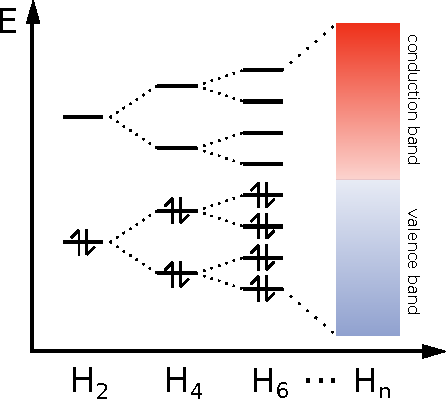
\includegraphics[scale=0.8]{Pics/MOchain}
\caption{}
\end{subfigure}
\begin{subfigure}{0.45\linewidth}
\centering
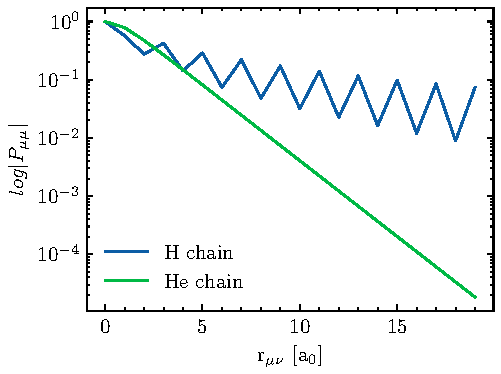
\includegraphics[scale=0.8]{density_decay}
\caption{}
\end{subfigure}
\caption{(a) Molecular orbital diagram for a hydrogen with increasing chain length. (b) Logarithm of the absolute value of the density matrix element $P_{\mu\nu}$ as a function of increasing distance $R_{\mu\nu}$ for a Hydrogen and a Helium atom chain.}
\label{fig:HCHAIN_DENSITY}
\end{figure}


%This sparsity relationship between two AOs is also known as Kohn's conjecture (ref DLMP2).
% exponential decay:
% Koh1959 https://journals.aps.org/pr/abstract/10.1103/PhysRev.115.809
% Ism1999 https://journals.aps.org/prl/abstract/10.1103/PhysRevLett.82.2127
% Goe1994 https://journals.aps.org/prl/pdf/10.1103/PhysRevLett.73.122
% Goe1998 https://journals.aps.org/prb/pdf/10.1103/PhysRevB.58.3501

% algebraic decay
% Tar2002 https://journals.aps.org/prb/abstract/10.1103/PhysRevB.66.233101

\subsection{Diagrammatic Notation}

Hollmann et al. \cite{Hol2017} have introduced a simple graphical representation to show contributing factors to the sparsity of a given matrix, tensor or tensor contraction. Each tensor index is represented as a vertex. Non-connected vertices each contribute $\mathcal{O}(N)$ elements to the overall expression. A sparsity relationship between two indices is represented as an \emph{edge} connecting two vertices. In that case, the number of \emph{pairs} scales as $\mathcal{O}(N)$. Consider the two electron integral tensor $\cn{\mu\nu}{\sigma\lambda}$. From the previous section, we know that the index pairs $\mu,\nu$ and $\lambda,\sigma$ are related by overlap. The diagrammatic representation takes the form:
\begin{center}
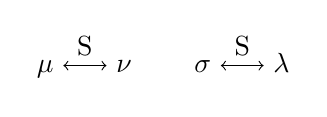
\begin{tikzpicture}

\snode{MU}{0,0}{\mu};
\snode{NU}{1,0}{\nu};
\snode{SIG}{2,0}{\sigma};
\snode{LAM}{3,0}{\lambda};

\draw[<->] (MU) -- (NU) node [midway, above] () {S};
\draw[<->] (SIG) -- (LAM) node [midway, above] () {S};

\end{tikzpicture}
\end{center}
\noindent There are two pairs of connected vertices, which indicates that the integrals can be evaluated with $\ccpx{2}$ effort, which is in agreement with the findings above. The $S$ denotes the overlap relationship between vertices.
For another example, consider the Hartree-Fock expression for the exchange matrix
\begin{equation}
K_{\mu\nu} = \cn{\mu\sigma}{\nu\lambda} P_{\lambda\sigma}
\end{equation}
\noindent Diagrammatically, the expression for $\mathbf{K}$ can be represented as
\begin{center}
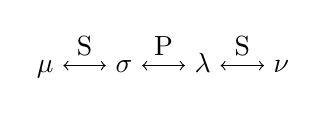
\begin{tikzpicture}

\snode{MU}{0,0}{\mu};
\snode{NU}{3,0}{\nu};
\snode{SIG}{1,0}{\sigma};
\snode{LAM}{2,0}{\lambda};

\draw[<->] (MU) -- (SIG) node [midway, above] () {S};
\draw[<->] (SIG) -- (LAM) node [midway, above] () {P};
\draw[<->] (LAM) -- (NU) node [midway, above] () {S};

\end{tikzpicture}
\end{center}
\noindent The connection between $\sigma$ and $\lambda$ is also known as a "P-junction" \cite{Nee2009}, which represents the sparsity relationship arising due to the exponential decay of density matrix elements. The sparsity graph is fully connected, which suggests that $\mathbf{K}$ can be evaluated with $\mathcal{O}(N)$ effort. This is indeed the case, as shown by the ONX or LinK method. For linear scaling to emerge, indices of an expression therefore need to be fully linked. This simple but important fact is also known the linked index rule (LIR). Diagrams also show which factors can influence the performance of the scaling, such as diffuseness of the atomic orbitals (slower S decay) or size of of the HOMO-LUMO gap (slower P decay). One can therefore conclude that the expression for $\mathbf{K}$ as given above, is less suitable for large basis sets and conducting systems.

\subsection{Rank Sparsity}

A positive semi-definite matrix $\mathbf{A}$ has the property that it can be decomposed as a product 
\begin{equation}
\mathbf{A} = \mathbf{B} \mathbf{B}^T
\end{equation}
\noindent where $\mathbf{A}$ has dimensions $N$ by $N$, and $\mathbf{B}$ has dimensions $N$ by $rank(A)$. The rank represents the number of linearly independent column vectors in matrix, and for $rank(A) < N$, the matrix is said to  be rank-deficient. The decomposition matrix $\mathbf{B}$ therefore is more compact and needs less storage space than $\mathbf{A}$. There are different ways to compute $\mathbf{B}$, such as Cholesky decomposition or QR decomposition.
The tensor $\cn{\mu\nu}{\sigma\lambda}$ can be represented as a $N_{AO}^2$
by $N_{AO}^2$0 matrix with combined row indices $I = \mu + N_{AO}*\nu$ and column indices $J = \sigma + N_{AO}*\lambda$. Because the tensor has been shown to be positive semi-definite, there also exists a decomposition, such that
\begin{equation}
\cn{\mu\nu}{\sigma\lambda} = A_{(\mu\nu)(\sigma\lambda)} = B_{(\mu\nu)X} B_{(\sigma\lambda)X}
\end{equation}
\noindent The rank of $\mathbf{A}$ is in general much smaller than the combined index range $N_{AO}^2$, and scales linearly rather than quadratically with the number of basis sets. The decomposition tensor $\mathbf{B}$ is therefore 3-dimensional, rather than 4-dimensional, which reduces the storage needed by an order of magnitude from $\ccpx{4}$ to $\ccpx{3}$, ignoring sparsity. In the limit of large molecules, the NZEs of $\mathbf{B}$ also scale with $\ccpx{2}$. Rather than for the molecular integrals in the AO basis, decomposition techniques are more useful for reducing the storage size of molecular integrals in the canonical MO basis
\begin{equation}
\cn{ia}{jb} = C_{\mu i} C_{\sigma a} B_{\mu \sigma X} B_{X \nu \lambda} C_{\nu j} C_{\lambda b} = B_{iaX} B_{Xjb}
\end{equation} 
\noindent The AO-MO transformation step is also drastically sped up, but remains a $\ccpx{4}$ effort. Rank sparsity has therefore little impact on the overall scaling, but rather reduces the scaling \emph{prefactor}. Over the years, different methods have been proposed to compute $\mathbf{C}$, such as density fitting, Cholesky decompostion, pseudo-spectral methods, or tensor hypercontraction.
Density matrices at different levels of theory (Hartree Fock, MP2, CC ...) also exhibit rank sparsity. Decomposition of such matrices play an important role in local molecular orbital schemes and low scaling electronic structure methods, as will be shown in later sections.

% pos def Roo1951 C. C. J. Roothaan, Rev. Mod. Phys., 23, 69 (1951).

% Schwarz inequality Has1989 https://onlinelibrary.wiley.com/doi/abs/10.1002/jcc.540100111

% Good explanation for "linked indices rule" https://aip.scitation.org/doi/pdf/10.1063/1.4926879

% Nee2009 https://reader.elsevier.com/reader/sd/pii/S0301010408005089?token=A38BA6311BBE21191E796ADD75EF1602618F281416BBB8E8C22D61B0C75DF4C02EF402A33375738162D7AA02AFAB8685&originRegion=eu-west-1&originCreation=20210707062425

\FloatBarrier

\section{Density Fitting}

The method of choice in this thesis for the decomposition of two-electron molecular integrals is \emph{density fitting} (DF), also known as \emph{resolution of the identity} (RI). For a brief exploration of other popular methods, the reader is referred to Annex \ref{app:ERIDECOMO}.  

\subsection{Basics of Density Fitting}

The two-electron integrals can be expressed in terms of the charge product densities $\rho_{\mu\nu} = \chi_{\mu} \chi_{\nu}$ as
\begin{equation}
\cn{\mu\nu}{\sigma\lambda} = \int \int \frac{\rho_{\mu\nu}(\mathbf{r_1}) \rho_{\sigma\lambda}(\mathbf{r_2}) }{\mathbf{r_1} - \mathbf{r_2}} d\mathbf{r_1} d\mathbf{r_2}
\end{equation}
The charge densities $\rho$ can be approximated by fitting them to a set of atom-centered auxiliary functions $\chi_P$
\begin{equation}
\rho_{\mu\nu}(\mathbf{r}) = C_{P\mu\nu} \chi_{P}(\mathbf{r}) + \Delta \rho_{\mu\nu}
\end{equation}
\noindent Or in the chemist's notation:
\begin{equation}
\cket{\mu\nu} = C_{P\mu\nu} \cket{P} + \cket{\eps_{\mu\nu}} = \cket{\swtilde{\mu\nu}} + \cket{\eps_{\mu\nu}}
\label{eq:DFAPPROX}
\end{equation}
\noindent where $C_{P\mu\nu}$ are the fitting coefficients, and $\Delta \rho_{\mu\nu}$ or $\cket{\eps_{\mu\nu}}$ is the error introduced by the fitting procedure. Equation \ref{eq:DFAPPROX} is known as the density fitting approximation \cite{Whi1973,Bae1973,Vah1993,Sky2000}. The two-electron integrals then take the form
\begin{equation}
\begin{split}
\cn{\mu\nu}{\sigma\lambda} &= (\swtilde{\mu\nu}|\swtilde{\sigma\lambda}) +  \underbrace{(\swtilde{\mu\nu}|\eps_{\sigma\lambda}) + (\eps_{\mu\nu}|\swtilde{\sigma\lambda})}_\textrm{first order} + \underbrace{\cn{\eps_{\mu\nu}}{\eps_{\sigma\lambda}}}_\textrm{second order} \\
&= (\swtilde{\mu\nu}|\swtilde{\sigma\lambda}) + \eps_J^{(1)} + \eps_J^{(2)} 
\end{split}
\label{eq:DFERROR}
\end{equation}
\noindent Here, $\eps_J^{(1)}$ and $\eps_J^{(2)}$ represent the first order (linear) and second order (quadratic) error. The fitting coefficients are then generally found by minimizing $\eps_J^{(2)}$. Substituting $\scbra{\eps_{\mu\nu}} = \scbra{\mu\nu - \swtilde{\mu\nu}}$ gives
\begin{equation}
\frac{\partial}{\partial C^P_{\mu\nu}} \scn{\mu\nu - \swtilde{\mu\nu}}{\sigma\lambda - \swtilde{\sigma\lambda}} = 0
\end{equation}
\noindent which then yields a set of linear equations
\begin{equation}
\scn{\mu\nu}{P} - \sum_Q C^Q_{\mu\nu} \scn{Q}{P} = 0 
\label{eq:DFLLS}
\end{equation}
\noindent Finding the fitting coefficients by minimizing $\eps_J^{(2)}$ has the important feature that $eps_J^{(1)} = 0$, which can be shown by substituting Equation \ref{eq:DFLLS} back into Equation \ref{eq:DFERROR}. The total electron integral error is therefore \emph{quadratic} in the fitting error. Fitting procedures where the coefficients $C^P_{\mu\nu}$ satisfy Equation \ref{eq:DFLLS} are termed $\emph{robust}$ \cite{Dun2000}. Any restrictions posed on $C^P_{\mu\nu}$ makes $\eps_{1}$ different from zero and the error scales linearly. 
Equation \ref{eq:DFLLS} requires the evaluation of the three-centre-two-electron (3c2e) and two-centre-two-electron (2c2e) integrals in the auxiliary basis set $\{P\}$
\begin{equation}
\cn{\mu\nu}{P} = \int \int \chi_{\mu}(\mathbf{r_1}) \chi_{\mu}(\mathbf{r_1}) \frac{1}{\mathbf{r_1} - \mathbf{r_2}} \chi_{P}(\mathbf{r_2}) d\mathbf{r_1} d\mathbf{r_2} 
\end{equation}
\begin{equation}
\cn{P}{Q} = \int \int \chi_{P}(\mathbf{r_1}) \frac{1}{\mathbf{r_1} - \mathbf{r_2}} \chi_{Q}(\mathbf{r_2}) d\mathbf{r_1} d\mathbf{r_2} 
\end{equation}
\noindent The fitting coefficients are generally computed by inverting $\cn{P}{Q}$, which leads to the following approximation for the four-center-two-electron integrals (4c2e)
\begin{equation}
\cn{\mu\nu}{\sigma\lambda} \approx \cn{\mu\nu}{P} \cn{P}{Q}^{-1} \cn{Q}{\sigma\lambda}
\end{equation}
\noindent Matrix inversion is a $\ccpx{3}$ computational effort. For more details on precision and best practices involving matrix inversion, see Annex \ref{app:MATINV}.
% Introduced independently by
% (Coulomb) Whi73 https://aip.scitation.org/doi/10.1063/1.1679012
% (Overlap) Bae1973 https://doi.org/10.1016/S0301-0104(99)00271-2 2, 41 (1973).
% Dunlap improved Baerends by using coulomb instead of overlap
% Dun1979 https://aip.scitation.org/doi/pdf/10.1063/1.438728
% Dun1979a https://doi.org/10.1063/1.438313 71, 4993 (1979).
% Begriff "Robust" erstmals hier
% Dun2000 https://www.sciencedirect.com/science/article/pii/S0166128099004339?via%3Dihub

\subsection{Scaling of the 3c2e Integrals}

Using the diagrammatic representation introduced earlier, the 3c2e integral tensor reduces to
\begin{center}
\begin{tikzpicture}
\snode{MU}{0,0}{\mu};
\snode{NU}{1,0}{\nu};
\snode{X}{2,0}{P};
\draw[<->] (MU) -- (NU) node [midway, above] () {S};
\end{tikzpicture}
\end{center}
The number of non-zero elements therefore scales as $\ccpx{2}$, just like for the 4c2e integrals. Similarly, the Schwarz inequality can be used to screen out small integrals
\begin{equation}
\left\lvert \cn{\mu\nu}{P} \right\rvert \leq \left\lvert \cn{\mu\nu}{\mu\nu} \right\rvert^{1/2} \left\lvert \cn{P}{P} \right\rvert^{1/2}
\end{equation}
\noindent As mentioned above, Schwarz screening does not take into account increasing bra-ket distance. The long-range decay is too slow to be of any advantage in the case of the 4c2e integrals. However, it was found \cite{Hol2015} that for an auxiliary density $\chi_P(\mathbf{r}$ with angular momentum $l_P$, the 3c2e integrals actually decay as $1/R^{-1 - l_P}$ with increasing bra-ket distance, establishing a weak but not insignificant sparsity relationship between $\cbra{\mu\nu}$ and $\cket{P}$ 
\begin{center}
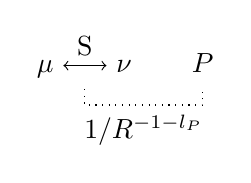
\begin{tikzpicture}
\snode{MU}{0,0}{\mu};
\snode{NU}{1,0}{\nu};
\snode{MUNU}{0.5,0}{};
\snode{X}{2,0}{P};
\draw[<->] (MU) -- (NU) node [midway, above] () {S};
\draw[dotted] (MUNU.south) |- (1.25, -0.5) node [below]{$1/R^{-1-l_P}$} -| (X.south);
\end{tikzpicture}
\end{center}
\noindent In principle, the 3c2e integrals can be evaluated with linear effort. Hollmann et al. \cite{Hol2015} have introduced a tight upper bound, known as the SVQl estimator, to exploit this faster decay. Due to the dependence on $l_P$, the screening is most effective with larger basis sets with high angular momentum functions.

The fitting coefficients evaluated as $C^P_{\mu\nu} = \cn{\mu\nu}{Q} \cn{Q}{P}^{-1}$ formerly scale with $\ccpx{3}$
\begin{center}
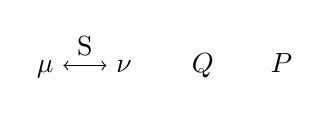
\begin{tikzpicture}
\snode{MU}{0,0}{\mu};
\snode{NU}{1,0}{\nu};
\snode{Q}{2,0}{Q};
\snode{P}{3,0}{P};
\draw[<->] (MU) -- (NU) node [midway, above] () {S};
\end{tikzpicture}
\end{center}
\noindent due to the inverse of $\cn{P}{Q}$ not being sparse. 

\subsection{Local Density Fitting: Principles} 
The long-range behaviour introduced by Equation \ref{eq:DFLLS} is often deemed "unphysical" \cite{Tew2018}. \emph{Local density fitting} (LDF) methods circumvent this problem by forcing a more rapid decay of long-range contributions, either (a) by using a different metric in the fitting procedure or (b) by constructing domains $[\mu\nu]$ that exclude distant fitting functions $P$ a priori. In both cases, Equation \ref{eq:DFLLS} no longer holds and the error in the electron integrals increases linearly with the fitting error. Therefore, the density fitting procedure is no longer robust. Fortunately, LDF methods can use a different expression for the electron integrals which includes the first order terms to remove the linear error
\begin{equation}
\cn{\mu\nu}{\sigma\lambda} \approx (\widetilde{\mu\nu}|\sigma\lambda) + (\mu\nu|\widetilde{\sigma\lambda}) - (\widetilde{\mu\nu}|\widetilde{\sigma\lambda})
\label{eq:DUNLAP}
\end{equation}
\noindent which is known as Dunlap's robust density fitting formula \ref{Dun2000}. It greatly increases accuracy for LDF. 
 
\subsection{LDF (I): Short-Range Metrics}
The first type of LDF methods replaces the fitting procedure in the Coulomb metric in Equation \ref{eq:DFLLS} by a more general expression
\begin{equation}
B_{\mu\nu}^{P} - C_{\mu\nu}^{Q} M_{QP} = 0
\end{equation}  
\noindent where $B_{\mu\nu}^{P}$ and $M_{PQ}$ are the 3c2e and 2c2e integrals given by
\begin{equation}
B_{\mu\nu}^P = \int\int \bfun{\mu}{1}\bfun{\nu}{1} g(\mbf{r_1},\mbf{r_2}) \bfun{P}{2} d\mbf{r_1} d\mbf{r_2}
\end{equation}
\begin{equation}
M_{PQ} = \int\int \bfun{P}{1} g(\mbf{r_1},\mbf{r_2}) \bfun{Q}{2} d\mbf{r_1} d\mbf{r_2}
\end{equation}
\noindent with $g$ being the operator for the local metric. A list of known local metrics is given in Table \ref{tab:DFMETRICS}. Earliest forms of density fitting actually first used an overlap metric to directly minimize the norm of the residual $R_{\mu\nu} = \cbra{\mu\nu} - \cbra{\widetilde{\mu\nu}}$ by the linear least squares methods \cite{Bae1973}, and the fitting coefficients are computed as
\begin{equation}
C^P_{\mu\nu} = S_{PQ}^{-1} (\mu\nu Q)
\label{eq:OVLPMET}
\end{equation}
\noindent where $S_{PQ}$ is the overlap matrix of the auxiliary basis, and $(\mu\nu Q)$ are the 3-center-\textbf{1-electron} overlap integrals. While the overlap metric has the most rapid decay and the quantities in Equation \ref{eq:OVLPMET} can be evaluated in $\mathcal{O}(N)$ time, it has the worst accuracy of all metrics. One solution to this problem is to introduce a metric which is intermediate between overlap and coulomb fitting. Examples include the Yukawa, Coulomb- and Gaussian-attenuated metrics. These intermediate metrics introduce a damping factor $\omega$ to control the sparsity and accuracy of the density fit. In the limit where $\omega \rightarrow 0$, and $\omega \rightarrow \infty$, one recovers the coulomb and overlap metric, respectively. Figure \ref{fig:DFMETRICS} shows the decay behaviour of the Coulomb-attenuated metric, for $\omega$ = 0.01, 0.1 and 1.0, compared to the overlap and the Coulomb metric. 

\begin{table}
\centering
\begin{tabular}{cc}
\hline
Metric & $g(r_{12})$ \\ \hline
\multirow{2}{*}{Overlap \cite{Bae1973}} & \multirow{2}{*}{1} \\ & \\
\multirow{3}{*}{Coulomb-Attenuated \cite{Jun2005}} & \multirow{3}{*}{$\dfrac{erfc(\omega r_{12})}{r_{12}}$} \\ & \\ & \\
\multirow{3}{*}{Yukawa \cite{Gil2005}} & \multirow{3}{*}{$\dfrac{e^{-\omega r_{12}}}{r_{12}}$} \\ & \\ & \\
\multirow{3}{*}{Gaussian-Damped \cite{Rei2008}} & \multirow{3}{*}{$\dfrac{e^{-\omega r_{12}^2}}{r_{12}}$} \\ & \\ & \\ \hline
\end{tabular}
\caption{Expressions for the operator $g$ in different local metrics.}
\label{tab:DFMETRICS}
\end{table}

\begin{figure}
\centering
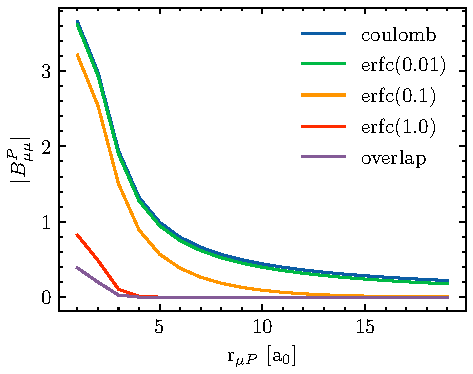
\includegraphics[scale=1.0]{ldf.pdf}
\caption{Absolute value of the 3c2e integral $B_{\mu\mu P}$ between two 1s GTOs $\mu$ and $P$ with $\alpha$ = 1.0 using different metrics.}
\label{fig:DFMETRICS}
\end{figure}

% A:
% Bae1973 https://www.sciencedirect.com/science/article/pii/030101047380059X?via%3Dihub
% Vah1993 https://www.sciencedirect.com/science/article/pii/0009261493891517?via%3Dihub
% Sky2000 https://www.sciencedirect.com/science/article/pii/S0166128099004340?via%3Dihub
% B: Jun2005 https://www.pnas.org/content/102/19/6692 
% C: Gil2005 https://aip.scitation.org/doi/10.1063/1.2000867 
% D: Rei2008 https://aip.scitation.org/doi/10.1063/1.2956507

% Hol2015 D.S. Hollman, H.F. Schaefer, and E.F. Valeev, J. Chem.Phys.142(2015)

\subsection{LDF (II): Local Domains}

The second method to force locality in density fitting consists in constructing local domains for each atom, pair of atoms or local molecular orbital, and excluding any auxiliary functions that lie outside, which can drastically reduce the dimension of the fitting procedure. 

\subsubsection{Atomic Resolution of the Identity}

The simplest example of a domain is one that includes a single atom. The atomic resolution of the identity (ARI) \cite{Sod2008} uses a fitting procedure where the sum over auxiliary function $Q$ only includes those which are centered on the same atom $A$ as the atomic orbital $\mu$
\begin{equation}
\cket{\widetilde{\mu\nu}} = \sum_{Q \cup A_{\mu}} \cn{P}{Q}_{A_{\mu}}^{-1} \cn{\mu\nu}{Q}
\end{equation}
\noindent Each atom $X$ has its own metric matrix inverse $\cn{P}{Q}_X^{-1}$ which takes the form 
\begin{equation}
\cn{P}{Q}_X^{-1} = B_X \left( \cn{P}{Q}_D + B_X \cn{P}{Q}_{OD}B_X\right)^{-1}B_X
\end{equation}
\noindent where $\cn{P}{Q}_D$ and $\cn{P}{Q}_{OD}$ are the diagonal and off-diagonal part of $\cn{P}{Q}$ respectively. $B_X$ is a so-called \emph{bump matrix} which imposes a fast, but smooth decay between functions $P$ and $Q$ in order to avoid using all functions $P$ for the fitting. For further details, the reader is referred to the original publication. The bump matrix uses multiple distance-dependent criteria which make the ARI less of a black-box method.

% Sod2008 https://aip.scitation.org/doi/pdf/10.1063/1.2828533

\subsubsection{Pair-Atomic Resolution of the Identity}

A more popular and simple variant of atomic density fitting is the pair-atomic resolution of the identity (PARI) method \cite{Mer2013}. As the name implies, the domains include atom \emph{pairs} rather than a single atom. Again expressing it in terms of the fitting procedure
\begin{equation}
\cn{P}{\mu\nu} = \sum_{Q \in A \cup B} \cn{P}{Q} C^Q_{\mu\nu} \quad \forall P \in A \cup B
\end{equation}
\noindent The number of linear equations is equal to the number of non-zero pairs $\mu\nu$, which scales linearly. However, the PARI approach enforces heavy constraints on the fitting coefficients, which leads to large integral errors. Merlot et al. proposed to increase the atomic pair domain with any atoms which lie between A and B. Alternatively, larger and more diffuse basis sets can be used. In both cases, performance is sacrificed for increased accuracy. The absence of any distance dependent parameters or thresholds still make it an attractive method both for Hartree Fock and Post-Hartree Fock methods \cite{Man2015,For2020}.

% Mer2013 https://onlinelibrary.wiley.com/doi/full/10.1002/jcc.23284

\subsubsection{LDF using Local Molecular Orbitals}

Finally, domains can also be formed using local molecular orbitals instead of AOs. LMOs are larger than AOs, but are still generally centered on only a few atoms. The exact atomic sites can be determined for example by using a Mulliken population analysis. Consider the density fitting procedure as proposed by Polly et al. for their LDF-Hartree Fock method \ref{Pol2004}
\begin{equation}
\cn{\mu i}{P} = \sum_{Q \in [i]_{fit}} \cn{P}{Q} C^Q_{\mu i}
\end{equation}
The fitting coefficients are determined individually for each AO-LMO pair $\cket{\mu i}$, and include only those auxiliary functions centred on atoms in the fitting domain $[i]_{fit}$ for which the Mulliken charges are above a given threshold. Although the fitting coefficients need to be recomputed for each update of the MO coefficients, the number of $\cket{\mu i}$ pairs scales linearly with system size. This type of local density fitting and variations thereof are predominantly used in pair-orbital specific local correlation methods, and will be explained in more detail further below. 

% Pol2004 Fast Hartree–Fock theory using local densityfitting approximations

\subsection{LDF (III): Quasi-Robust Density Fitting}

Local density fitting imposes constraints on the fitting procedure, and the integral error consequently scales linearly with the fitting error. Using Dunlap's robust formula is deemed necessary in most cases to achieve acceptable accuracy, but reintroduces the slowly decaying 3c2e integrals. Furthermore, replacing the 4c2e integrals by Equation \ref{eq:DUNLAP} greatly increases the complexity of expressions in electronic structure theory, which is still manageable for ground state methods, but quickly becomes cumbersome for excited states.

Quasi-robust density fitting (QRDF) \cite{Tew2018} aims to combine the exponential decay behavior of LDF with an accuracy comparable to standard density fitting, without the use of Dunlap's formula. Again, consider the fitting procedure 
\begin{equation}
\sum_Q \cn{P}{Q} C^Q_{\mu\nu} = \cn{P}{\mu\nu}
\end{equation}
\noindent The sets of auxiliary functions $\{P\}$ and $\{Q\}$ have different roles. The functions $Q$ fit the charge density $\cket{\mu\nu}$, while the $P$ functions act as \emph{test functions} where the electron integrals should be accurate, i.e. where $\cn{X}{\widetilde{\mu\nu}} \approx \cn{X}{\mu\nu}$. For two functions $\mu$ and $\nu$ not located on the same atom, their charge density $\cket{\mu\nu}$ lies in the vacuum between them, and the atom-centered auxiliary functions may be ill-suited to fit $\cket{\mu\nu}$. For this reason, the fitting procedure draws from all fitting functions $\{P\}$ spanning the whole molecule to cancel out the linear error, which in consequence introduces long-range contributions in $C_{\mu\nu}^P$ in the coulomb metric, even if $\cket{P}$ is not close to $\cket{\mu\nu}$. 
The basic idea of QRDF is to only chose fitting functions $\{P\}$ close to $\cket{\mu\nu}$ via overlap criteria, but still perform the fitting procedure in the coulomb metric.

\subsubsection{The QRDF Fitting Procedure}

For a set of given $\mu,\nu$, select a set of \emph{fitting function} $\{P_{\mu\nu}\} \in \{P\}$ close to $\cket{\mu\nu}$ according to the criteria
\begin{equation}
\left\lvert \sum_R S_{PR}^{-1} (R\mu\nu) \right\rvert > T 
\label{eq:QRDF_FIT}
\end{equation} 
\noindent where $S$ is the auxiliary overlap matrix, and $(R\mu\nu)$ are the 3-centre-1-electron overlap integrals. Next, choose a set of test functions $\{Q_{\mu\nu}\} \in \{P\}$ using
\begin{equation}
f(Q_{\mu\nu},P_{\mu\nu}) < R
\label{eq:QRDF_TEST}
\end{equation}
\noindent with
\begin{equation}
f(A,B) = \frac{\alpha \beta}{\alpha + \beta} \left\lvert \mathbf{A} - \mathbf{B} \right\rvert^2
\end{equation}
\noindent where for two auxiliary functions $A$ and $B$, the values $\alpha$, $\beta$ are their smallest primitive exponents and $\mathbf{A}$, $\mathbf{B}$ are their respective positions. The fitting coefficients are then determined via
\begin{equation}
\sum_P \cn{Q_{\mu\nu}}{P_{\mu\nu}} C^P_{\mu\nu} = \cn{Q_{\mu\nu}}{\mu\nu}
\label{eq:QRDFLLS}
\end{equation}
\noindent where the fitting coefficients are accurate within the set of test functions $\{Q_{\mu\nu}\}$. The linear equations in Equation \ref{eq:QRDFLLS} can be solved via QR decomposition or singular value decomposition (SVD) of the rectangular matrix $\cn{Q_{\mu\nu}}{P_{\mu\nu}}$.
The QRDF scheme depends on two parameters, $T$ and $R$. In the limit where $T \rightarrow 0$ and $R \rightarrow \infty$, the standard fitting procedure in the coulomb metric is recovered. 

The fitting functions $\{P_{\mu\nu}\}$ are selected via overlap criteria and therefore scale linearly with the number of pairs $\cket{\mu\nu}$, and consequently the same holds true for the number of test functions $\{Q_{\mu\nu}\}$ close to $\{P_{\mu\nu}\}$ chosen by Equation \ref{eq:QRDF_FIT}. In the limit of large molecules, the size of the rectangular matrix in Equation \ref{eq:QRDF_TEST} becomes constant and the fitting procedure can be evaluated with $\mathcal{O}(N)$ effort. However, a QR decomposition needs to be computed for each set of $\cket{\mu\nu}$, leading to relatively high prefactor which makes the method not competitive for dense 3D structures like water clusters, as will be discussed in the results section.
The QRDF method has been shown to deliver accuracies comparable to standard density fitting, without the use of Dunlap's formula, making it a very attractive alternative to other LDF schemes, especially if one wishes to reduce the complexity of expressions involving LDF.

\subsection{Auxiliary Basis Sets}

The density fitting approximation does not make any assumptions about the size or shape of the auxiliary basis set used. In principle, the fit is exact for the basis set containing all $N_{AO}^2$ Gaussian products $\chi_P = \chi_{\mu} \chi_{\nu}$. In practice, the product space is over-complete and can be represented by much smaller basis sets. Accurate results can be obtained for auxiliary basis sets which are about 4 times larger than the principal basis set they are used with. 

Auxiliary basis sets generally need more higher angular momentum functions than standard basis sets. Consider an isolated, unperturbed atom, with electrons occupying atomic orbitals with highest angular momentum $l_{occ}$. A minimal basis set for this atom contains functions of angular momenta 0 to $l_{occ}$. However, a minimal auxiliary basis set for fitting the product space $\chi_{\mu}^{0...l_{occ}} \chi_{\nu}^{0...\l_{occ}}$ needs functions with maximum angular momentum $2l_{occ}$. For example, 2nd row elements ($l_{occ}$ = 1) need an auxiliary basis set containing d-functions, and first row transition metals ($l_{occ}$ = 2) even need g-functions. Similarly to standard basis sets, to describe atoms in molecules where the orbitals are subject to polarization effects, even higher angular momentum functions are needed to fit polarization functions. In practice, a principal basis set with maximum angular momentum $l_{bas}$ is paired with an auxiliary basis set with highest angular momentum $l_{bas} + l_{occ}$. 

Auxiliary basis sets have the drawback of being method-specific. There are two categories: auxiliary basis sets for density fitted Hartree-Fock (DF-HF) and for density fitted correlated methods (e.g. DF-MP2, DF-CCSD, DF-ADC(2)). Auxiliary basis sets for DF-HF not only need to reproduce Hartree Fock energies, but also need to minimize negative impact on post-Hartree methods. An ill-suited auxiliary basis set leads to a deterioration of the virtual orbital space, and hence an increased error for correlated methods. 

Optimization procedures often try to minimize the energy differences between the standard method and its density fitting approximation in a series of atomic calculations. For example, the jkfit family of basis sets (cc-pVXZ-JKFIT \cite{Wei2002}, def-XVP-JKFIT \cite{Wei2008}) minimize the error
\begin{equation}
\Delta E_{HF} = E_{HF} - E_{DF-HF}
\end{equation}
The RI basis set family (cc-pVXZ-RIFIT \cite{Wei1998}, def2-XVP-RIFIT \cite{Ber1998}) minimizes the same energy difference but for MP2 or Coupled Cluster. 

Another disadvantage of auxiliary basis sets is that the accuracy of the fitting procedure cannot be easily controlled as a function of its composition (number of functions, angular momenta...), but rather extensive benchmarks are needed for each basis set that is introduced. An alternative approach was proposed by Aquilante et al. \cite{Aqu2007} where the fitting basis sets are generated automatically by Cholesky decomposition of the atomic 2-electron integrals
\begin{equation}
\cn{\mu\nu}{\sigma\lambda} = L^X_{\mu\nu} L^X_{\sigma\lambda}
\end{equation}
\noindent The Choleksy vectors $\mathbf{L}_{\mu\nu}$ indicate which product densities should be taken to construct the auxiliary basis. This type of atomic Cholesky decomposition (aCD) basis sets has the advantage that the accuracy can be rigorously controlled by the decomposition threshold $\theta$. To remove linear dependencies in the aCD basis set, another Cholesky decomposition can be performed to yield the atomic compact Cholesky decomposition (acCD) auxiliary basis set \cite{Aqu2009}.

% Dunning JKFIT (1): Wei2002 https://pubs.rsc.org/en/content/articlepdf/2002/cp/b204199p
% Karlsruhe JKFIT (2): Wei2007 https://onlinelibrary.wiley.com/doi/full/10.1002/jcc.20702
% MP2 Karlsruhe Wei1998 https://www.sciencedirect.com/science/article/pii/S0009261498008628
% Dunning (MP2) Ber1998 https://aip.scitation.org/doi/pdf/10.1063/1.476732
% Aqu2007 https://aip.scitation.org/doi/10.1063/1.2777146
% Aqu2009 https://aip.scitation.org/doi/10.1063/1.3116784

\section{Multipole Expansion of the Electron Integrals}

The slow $1/R$ between the product densities $\Omega_{\mu\nu}$ and $\Omega_{\lambda\sigma}$ in the coulomb integrals is a major obstacle for achieving linear scaling in cases where no other sparsity relationship can be established between indices belonging to separate charge densities, e.g. in the evaluation of the coulomb matrix $\mathbf{J}$ versus the exchange matrix $\mathbf{K}$. Luckily, there are approximate methods for integral evaluation that can be computed with $\mathcal{O}(N)$ effort, known as \emph{multipole methods}.

\subsection{Classical and Non-Classical Electron Integrals}

First, consider the concept of classical and non-classical interactions. Two electron integrals are said to be \emph{non-classical} if the two charge densities $\Omega_{\mu\nu}$ and $\Omega_{\sigma\lambda}$ overlap, and \emph{classical} if the charge densities are well separated. In the latter case, the electron integrals represent classical interactions between disjoint point charges, and can be approximated using multipole methods, whereas the non-classical contributions must be evaluated using the more expensive standard integral codes such as McMurchie-Davidson or Obara-Saika. 

Two Gaussian distributions $\Omega_P$ and $\Omega_Q$ are considered \emph{well-separated} up to a target accuracy 10$^{-k}$, if their center-to-center distance $R_{PQ}$ is larger than the sum of their extents $ext_P$ and $ext_Q$:
\begin{equation}
R_{PQ} > ext_P + ext_Q
\end{equation} 
\noindent with the extent of a Gaussian product $P$ defined as 
\begin{equation}
r_P = \frac{1}{\sqrt{p}} erfc^{-1}(10^{-k})
\end{equation}
\noindent where $p$ is the reduced exponent. Another important thing to note is that the number of significant non-classical and classical integrals scale as $\mathcal{O}(N)$ and $\ccpx{2}$ respectively \cite{Hel2000}, which has important consequences as will be shown further below. 

\subsection{Multipole Expansion}

For two well-separated charge distributions $P$ and $Q$, the inverse inter-electronic distance can be expanded in terms of Legendre polynomials $\mathcal{P}$ as
\begin{equation}
\frac{1}{r_{12}} = \sum_{l=0}^{\infty} \frac{\Delta r_{12}^l}{R_{PQ}^l} \mathcal{P}_{l} cos \theta
\label{eq:PARTIALWAVE}
\end{equation}
\noindent with 
\begin{equation}
cos \theta = \frac{\Delta \mathbf{r}_{12}^l \mathcal{R}_{QP}}{\Delta r_{12} R_{QP}} 
\end{equation}
\begin{equation}
\Delta \mathbf{r}_{12} = \mathbf{r}_{1P} \mathbf{r}_{2Q}
\end{equation}
\noindent where $\mathbf{r}_{1P}$ and $\mathbf{r}_{2Q}$ are the distance between electron 1,2 and the centers $P$,$Q$. Equation \ref{eq:PARTIALWAVE} is also known as the partial-wave expansion of the coulomb operator \cite{Arf2012}. Plugging Equation \ref{eq:PARTIALWAVE} into the expression for the two-electron repulsion integrals gives the bipolar multipole expansion of the two-electron integrals
\begin{equation}
g_{abcd} = \sum_{l=0}^{\infty} \sum_{m=-l}^l \sum_{j=0}^{\infty} \sum_{k=-j}^{j} M_{ab}^{lm}(P) T_{lm,jk} M_{cd}^{jk}
\end{equation}
\noindent where $\mathbf{M}_{ab}^{lm}(P)$ is the multipole moment of the charge distribution $P$ with total moment $l+k$, and $\mathbf{T}$ is the so-called interaction matrix. As such, the complicated 6-dimensional evaluation of $g$ can be simply substituted by two 3-dimensional integrations of the multipole moments $\mathbf{M}$ at a much lower cost. For the lowest order expansion, where $l$ = $m$ = 0, and $j$ = $k$ = 0, the multipole moments and the interaction matrix become 
\begin{equation}
M_{ab}^{00} = S_{ab}
\end{equation}
\begin{equation}
M_{cd}^{00} = S_{cd}
\end{equation}
\begin{equation}
T_{00,00} = 1/R_{PQ}
\end{equation}
\noindent The zero order term of the multipole expansion therefore takes the form
\begin{equation}
g_{abcd} \approx \frac{S_{ab}S_{cd}}{R_{PQ}}
\end{equation}

\subsection{Fast Multipole Method}

While the number of individual non-zero integrals still scales with $\ccpx{2}$, the total contribution of all pair-wise interactions to the total energy (Hartree Fock, MP2 ...), can actually be evaluated in $\mathcal{O}(N)$.

For the sake of simplicity, consider a system with point-charge particles with charge $Z$, in a 2-dimensional plane. The total interaction energy is given by
\begin{equation}
U = \sum_{i>j} \frac{Z_i Z_j}{r_{ij}}
\label{eq:INTERENERGY}
\end{equation}
\noindent Evaluating Equation \ref{eq:INTERENERGY} as is takes a quadratic effort. In a first approximation, one can divide the plane into a grid of blocks of equal size, where each block contains a certain number of particles (Figure \ref{fig:FMM1}). Consider the interaction of a single particle $i$ in its source block $C$ with the other particles in the system. The interaction has two contributions: near-field (NF) contributions $U_{NF}$ from the other particles in the source block, and the blocks immediately surrounding it, and far-field (FF) contributions $U_{FF}$ from boxes that are well-separated from $C$. The NF interactions are evaluated directly by summing over all particles $j$ in the near-field
\begin{equation}
U^{NF}_i = \sum_{j \in NF} \frac{Z_i Z_j}{R_{ij}}
\end{equation}
\noindent while FF interactions are computed using multipole expansions $\mathbf{q}_{iC}$ and $\mathbf{q}_A$ of the FF boxes and the particle $i$
\begin{equation}
U^{FF}_i = \sum_{A \in FF} \mathbf{q}_{iC} \mathbf{T}_{CA} \mathbf{q}_A
\end{equation}
\noindent While evaluating the interaction energy at block-level rather than particle-level can considerably reduce the prefactor, the cost of this \emph{single-level multipole method} is still quadratic, since for each particle $i$, there is a system-dependent number of FF boxes. The granularity of the blocks is the same, independent of how far away the blocks are. To achieve linear scaling, the crucial point to realize is that, the further one gets from the source block $C$, the smaller the single-particle interaction $U_i$ becomes, and the less accurately it actually needs to be evaluated. This means that the farther one moves away from C, the larger the FF boxes can be. For this reason, \emph{multi-level multipole methods} introduce a hierarchy of boxes (Figure \ref{FMM2}), where at level 0, the whole system is in a single box, and for each subsequent level, the field is divided into fourths. FF boxes that are closest to C are evaluated at the highest level/granularity $S$. The region of FF boxes sourrounding the closest FF boxes are then treated at a lower level $S-1$, and so on, until all interactions have been computed. Because the multipole expansion is evaluated for increasing box size, it can be shown that the total number of boxes is constant for a single particle $i$. This is the basic idea on which the \emph{Fast Multipole Method} (FMM) operates \cite{Gre1987,Gre1994,Din1992}, and it has quickly become one of the most important algorithms in scientific computing, as the problem of particle-particle interaction is not limited to the field of quantum chemistry. FMM can evaluate the total interaction energy $U$ with linear computational complexity.

\begin{figure}
\centering
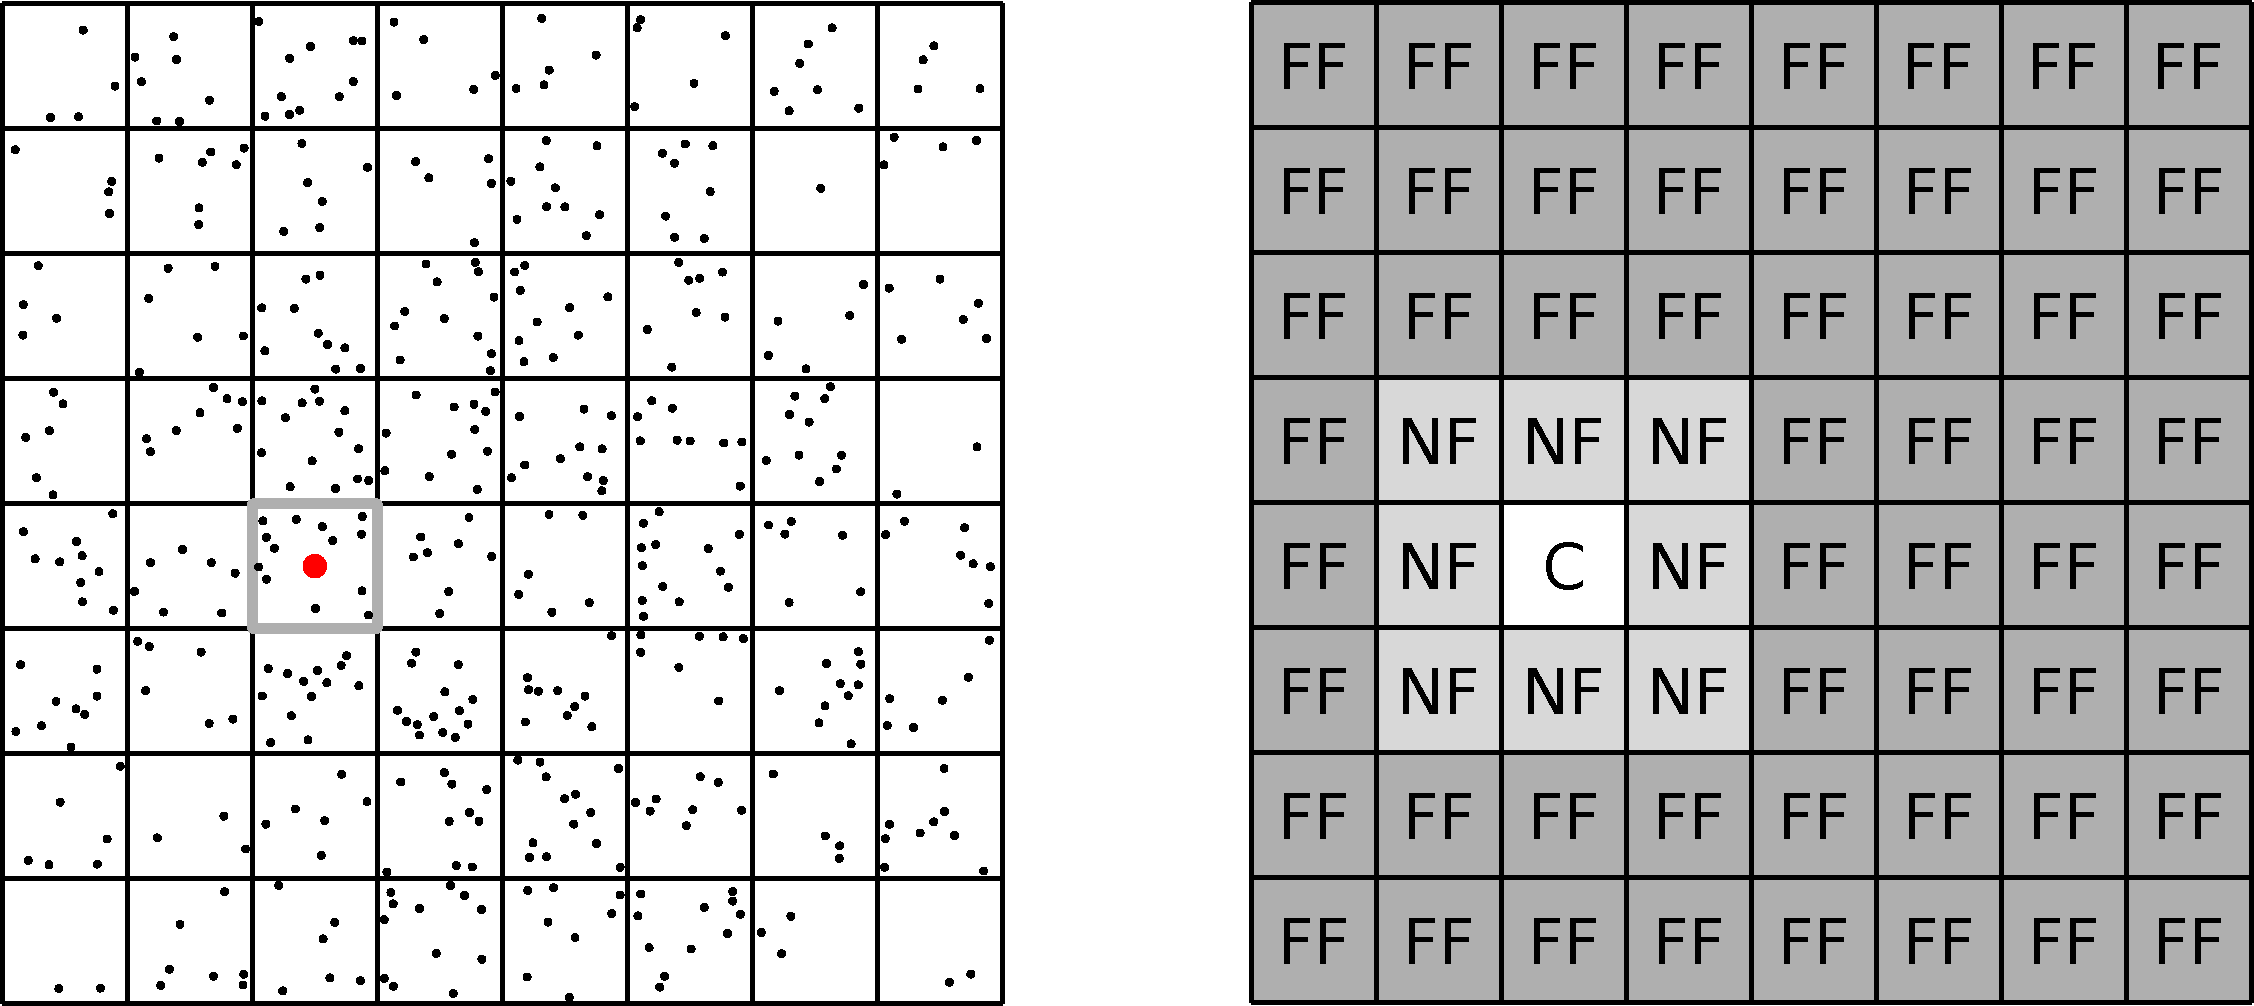
\includegraphics[scale=0.35]{Pics/FMM1}
\caption{In multipole methods, the system is subdivided into blocks of equal size containing one or more particles. For a reference block $C$, its surrounding blocks are categorized into near-field and far-field contributions which are treated using separate methods.}
\label{fig:FMM1}
\end{figure}

\begin{figure}
\centering
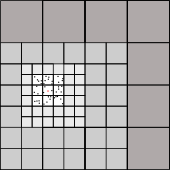
\includegraphics[scale=0.35]{Pics/FMM2}
\caption{In the fast multiple method, the granularity of the boxes becomes coarser the further away they are from the source blocks.}
\label{fig:FMM2}
\end{figure}

% Ark1970 https://www.sciencedirect.com/book/9780123846549/mathematical-methods-for-physicists
% Gre1987 L. Greengard and V. I. Rokhlin, J. Comput. Phys. 73, 325 (1987)
% Gre1994 L. Greengard, Science 265, 909, (1994)
% Din1992 H. Q. Ding, etc.... look at 28, 29 p. 426 big book

\subsection{Continuous Fast Multipole Method}

The fast multipole method does not work for continuous charge distrbutions like Gaussian functions, as their extents can be quite different from one another, making the separation into NF and FF contributions more difficult. Nonetheless, FMM has been generalized to the continous case, known as the continuous fast multipole method (CFMM) \cite{Whi1996}. The principle is the same as in multi-level multipole methods, only special care needs to be taken to only include classical contributions into the FMM treatment. For further details, the reader is referred to the original publication. 

\section{The ABCs of LMOs and NOs: Orbital Representations \label{sec:ABCLMO}}

To solve the Hartree-Fock equations in a computationally efficient way, it is favorable to choose the set of molecular orbitals such that they diagonalize the Fock matrix $\mbf{F}$. In other words, they are eigenfunctions of the Fock operator
\begin{equation}
\hat{f}\sket{\phi_i} = \eps_i \sket{\phi_i}
\end{equation} 
\noindent Here, $\{\phi_i\}$ are also known as the \emph{canonical molecular orbitals}. CMOs are not unique in the sense that there are infinitely many alternative molecular representations which yield the same electron density $\mathbf{P}$. Quantities like the total wave function energy or the electronic density are said to be \emph{orbitally invariant}. Non-observables like the MO energies are not preserved under orbital rotation. Let $\mbf{C}$ be the CMO coeffcient matrix. A new solution to the HF equations can then be generated by applying a unitary transformation such that
\begin{equation}
C^{new}_{\mu \olj} = U_{ji} C_{\mu i} \qquad \mbf{UU}\pdg = \mbf{1}
\end{equation} 
\noindent There are different reasons why one would want to use another MO basis: they can (a) offer a more intuitive picture for the interpretation of chemical phenomena and (b) help to achieve are more localized and compact representation of the wave function which is helpful for local correlation methods.

There are two significant types of molecular representations besides CMOs: local molecular orbitals (LMOs) and natural orbitals (NOs). The following sections will introduce both  types in more detail.

\subsection{Local Molecular Orbitals}

In contrast to canonical molecular orbitals, which are generally delocalized over the whole molecule, local molecular orbitals are confined to a relatively small volume and span only a few atoms (except in large conjugated systems). LMOs are well suited for a qualitative description of chemical reaction in terms of molecular bonds, lone pairs and $\pi$ systems \cite{Ste2019}. Moreover, they are often used in local correlation methods due to their reduced orbital span. There are several different ways for generating LMOs.

\subsubsection{LMOs by Reducing a Functional}
% (0) https://aip.scitation.org/doi/full/10.1063/1.2360264
% (1) https://journals.aps.org/rmp/abstract/10.1103/RevModPhys.32.296
% (2) https://journals.aps.org/rmp/abstract/10.1103/RevModPhys.35.457
% (3) https://aip.scitation.org/doi/10.1063/1.456588
% (4) J. E. Subotnik, Y. Shao, W. Z. Liang, and M. Head-Gordon, J. Chem. Phys. https://doi.org/10.1063/1.1790971 121, 9220 (2004).
% (5) https://aip.scitation.org/doi/10.1063/1.2033687

One of the most popular methods for finding LMOs consists in maximizing a localization function $\eta(\phi)$ by successive rotation of the orbital space. The most prominent examples are Foster-Boys (FB) \cite{Boy1960}, Edmiston-Ruedenberg (ER) \emph{Edm1963} and Pipek-Mezey (PM) \cite{Pip1989}. Their functionals can be written as

\begin{eqnarray}
\zeta_{FB}(\chi) = \sum_i \bra{\chi_i} \mathbf{r} \ket{\chi i}^2 \\
\zeta_{ER}(\chi) = \sum_i \cn{\chi_i \chi_i}{\chi_i \chi_i} \\
\zeta_{FB}(\chi) = \sum_i \sum_A \bra{\chi_i} \mathbf{P}_A \ket{\chi i}^2 
\end{eqnarray}

The problem is generally solved using an iterative procedure consisting in consecutive pair-wise rotations, known as Jacobi sweeps (Section \ref{sec:LOCORB}). These sweeps are repeated until convergence is reached, which may be slow. The methods differ within the procedure by how the rotational angle is computed, and scale differently with system size, with $\ccpx{3}$ for FB, $\ccpx{5}$ for ER and $\ccpx{4}$ for PM. A faster alternative to Jacobi sweeps does also exist \cite{Sub2004}. 

Over the years, PM has been the more popular choice of the three: like ER and unlike FB, it conserves $\sigma$-$\pi$ separation \cite{Aqu2006}, but scales more favorably than ER.

Functional localization methods are most often used for rotating occupied MOs. Virtual MOs are often plagued by convergence issues and have a steep computational cost simply due to being much more numerous than occupied MOs \cite{Sub2005}. It is crucial that molecular localization should not take longer than the methods they are used for, and hence VMOs are often localized using separate methods (e.g. PAO).

% EXAMPLES!! Ethylene (?)

\subsubsection{Projected Atomic Orbitals \label{sec:PAO}}
% (0) https://www.annualreviews.org/doi/10.1146/annurev.pc.44.100193.001241
% (1) https://aip.scitation.org/doi/full/10.1063/1.2173249

A set of highly localized molecular orbitals can be obtained by projecting the CMOs onto the atomic orbital basis, known as projected atomic orbitals (PAO) \cite{Sae1993}. For a set of orthonormal occupied and virtual molecular orbitals $\{\Psi_i\}$ and $\{\Psi_a\}$, the projection operators $\hat{P}$ and $\hat{Q}$ are defined as \cite{Chr2006}

\begin{eqnarray}
\hat{P} &= \ket{\Psi_i} \bra{\Psi_i} &= \ket{\chi_{\mu}} C_{\mu i} C_{\nu i} \bra{\chi_{\nu}} \\
\hat{Q} &= \ket{\Psi_a} \bra{\Psi_a} &= \ket{\chi_{\mu}} C_{\mu a} C_{\nu a} \bra{\chi_{\nu}}
\end{eqnarray}

\noindent which are then applied to the atomic orbitals $\chi$ 

\begin{eqnarray}
\hat{P} \ket{\chi_{\mu'}} &= \sum_{\mu} P_{\mu\nu} S_{\nu\mu'} \ket{\chi_{\mu'}} &= \sum_{\mu} \ovl{P}_{\mu \mu'} \ket{\chi_{\mu'}} = \ket{\chi_{\ulgm}} \\
\hat{Q} \ket{\chi_{\mu'}} &= \sum_{\mu} Q_{\mu\nu} S_{\nu\mu'} \ket{\chi_{\mu'}}  &= \ovl{Q}_{\mu \mu'} \ket{\chi_{\mu'}} = \ket{\chi_{\olgm}}
\end{eqnarray} 

The projection operators $\hat{P}$, $\hat{Q}$ and the non-symmetric PAO coefficient matrices $\mathbf{\ovl{P}}$, $\mathbf{\ovl{Q}}$ are \emph{idempotent}
\begin{equation}
\mbf{\ovl{P}}\mbf{\ovl{P}} = \mbf{\ovl{P}} \qquad
\mbf{\ovl{Q}}\mbf{\ovl{Q}} = \mbf{\ovl{Q}}
\end{equation}

\noindent and \emph{mutually orthogonal} 
\begin{equation}
\mbf{\ovl{P}}\mbf{\ovl{Q}} = \mbf{0} \qquad \mbf{\ovl{P}} + \mbf{\ovl{Q}} = \mbf{1} 
\end{equation} 

\noindent But not orthogonal within themselves
\begin{equation}
\sbraket{\chi_{\ulgm}}{\chi_{\ulgn}} = S^{PAO}_{\ulgm\ulgn} \qquad \bra{\chi_{\olgm}} \sket{\chi_{\olgn}} = S^{PAO}_{\olgm\olgn}
\end{equation}
\noindent Here, the indices $\ulgm,ulgn,...$ and $\olgm,\olgn,...$ are used for occupied and virtual projected atomic orbitals, respectively. The number of PAOs (occupied or virtual) is equal to the number of AOs, and are therefore linearly dependent (redundant). CMOs are transformed to PAOs by using
\begin{eqnarray}
\sket{\chi_{\ulgm}} &= (\mathbf{SC})_{\mu i}  \sket{\Psi_i} &= \ovl{C}_{\mu i} \ket{Psi_i} \\
\sket{\chi_{\olgm}} &= (\mathbf{SC})_{\mu a} \sket{\Psi_a} &=  \ovl{C}_{\mu a} \ket{\Psi_a}
\label{CMO2PAO}
\end{eqnarray}
\noindent The back-transformation is defined as
\begin{eqnarray}
\sket{\Psi_{i}} &= C_{\mu i} \sket{\ulgm} \\
\sket{\Psi_{a}} &= C_{\mu a} \sket{\olgn} 
\label{PAO2CMO}
\end{eqnarray}
PAOs are centred on the atom on which their corresponding AO is localized, but can still be delocalized over multiple atoms, depending on the sparsity of the density matrix. Methods which are entirely formulated in PAOs are rare but possible \cite{Chr2006}. The projection method is most often used on the virtual orbital space, where standrad localization procedures fail. In literature, the following alternative formular is often used for expression the virtual PAO coefficient matrix in terms of the occupied LMOs:
\begin{equation}
\mbf{\ovl{Q}} = \left( \mbf{1} - \mbf{LL}^{\dagger} \mbf{S} \right) \mbf{C} 
\end{equation}
\noindent where $\mbf{L}$ is the coefficient matrix of the occupied LMOs.

\subsubsection{Cholesky Molecular Orbitals}

Sparsity of the atomic density matrix is crucial for achieving low-scaling electronic structure methods. Aquilante et al. proposed \cite{Aqu2006} to define a set of occupied molecular orbitals by Cholesky decomposition of the density matrix. Analysis of the resulting Cholesky molecular orbitals (CholMOs) showed their localized character inherited from the sparsity of the density matrix.
\begin{equation}
\mathbf{P} = \mathbf{LL^T}
\end{equation}
Figure \ref{fig:LOCORB_CHOL} shows the sparsity of the occupied density matrix and the occupied Cholesky molecular coefficient matrix of the linear alkane H$_{322}$C$_{160}$. The number of CholMOs is equal to the rank of the density matrix, which is equal to the number of occupied orbitals. The CholMOs are computed by an incomplete Cholesky decomposition with full row and column pivoting (Section \ref{fig:CHOLDEC}. The unitary transformation matrix is given by

\begin{equation}
U_{i\uli} = C_{\mu i} S_{\mu \nu} L_{\nu \uli}
\end{equation}

The decomposition algorithm scales with $\ccpx{3}$ but can be made linearly scaling by using sparse matrix algebra. CholMOs have several advantages: the Cholesky decomposition is fast and non-iterative, and an initial guess for molecular orbitals is not needed. 

The scheme can be extended to virtual orbitals as well, by CD of the virtual atomic density matrix $\mathbf{Q}$. The rank of $\mathbf{Q}$ is equal to the number of virtual orbitals $n_vir$, therefore the prefactor of the incomplete CD increases with basis set size. Especially in the presence of diffuse functions, the rank reduction might not offer much of an advantage compared to simpler localization methods such as PAOs.  

Moreover, orbitals obtained by CD are less localized than FB or ER LMOs, especially for small molecules. Low scaling is still possible using CholMOs in the context of LMO correlation methods, albeit with a larger prefactor.

CD is also used in the context of AO-MP2 to reduce the prefactor of integral transformation by using the rank sparsity of the pseudo-density matrices, as will be shown further below. CholMOs can also used as an initial guess for iterative localization schemes to achive faster convergence.

\begin{figure}[h]
\centering
\begin{subfigure}{0.5\linewidth}
\centering
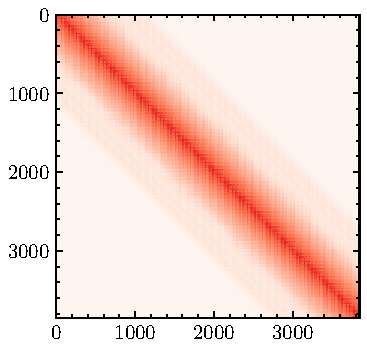
\includegraphics[scale=1.0]{densityO}
\end{subfigure}
$\Longrightarrow$
\begin{subfigure}{0.4\linewidth}
\centering
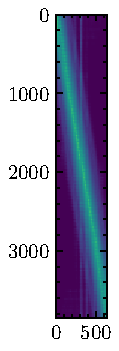
\includegraphics[scale=1.0]{choleskyO}
\end{subfigure}%
\hfill
\centering
\begin{subfigure}{0.5\linewidth}
\centering
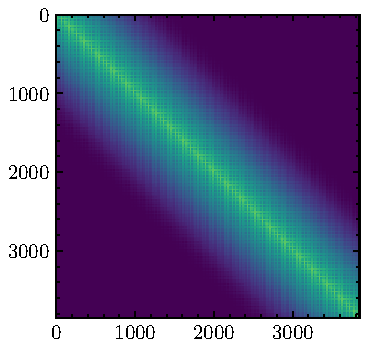
\includegraphics[scale=1.0]{densityV}
\end{subfigure}
$\Longrightarrow$
\begin{subfigure}{0.4\linewidth}
\centering
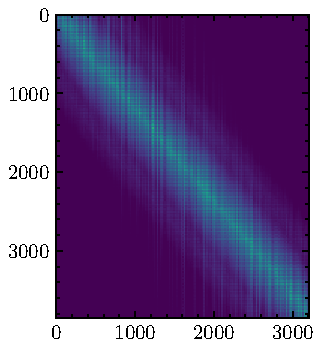
\includegraphics[scale=1.0]{choleskyV}
\end{subfigure}%
\caption{Cholesky decomposition, the occupied and virtual density matrices (left) yields a set of coefficients that describe a localized MO basis in the orbital and virtual space, respectively (right). The matrices are represented in terms of a heat map which inidicates the magnitude of $log_{10}(abs(a_{ij}))$.}
\label{fig:LOCORB_CHOL}
\end{figure} 

\subsection{Natural Orbitals}

While the schemes described above try to generate a set of occupied and/or virtual molecular orbitals localized in space, natural orbital (NOs) methods try to generate a set of "compact" orbitals, i.e. a minimal set of orbitals that can describe the problem at hand. The concept of natural orbitals was first introduced by Löwdin \cite{Low1956}. The natural orbitals $\Theta_i$ of a wave function $\Psi$ are defined as the eigenfunctions of the one-particle density operator $\hat{n}$

\begin{equation}
\hat{n}\ket{\Theta_i} = n_i \ket{\Theta_i} 
\end{equation}

\noindent where $n_i$ are the occupation numbers of the associated orbital $\Theta_i$. One can then choose a reduced orbital space $\{\tilde{\Psi}_i\}$ by only taking into account those orbitals with an occupation number above a certain threshold $\tau$. The orbitals are "natural" in the sense that they are determined purely using $\Psi$, and are intrinsic to the system. NOs are computed by diagonalizing the one-particle density matrix at the desired level of theory (Hartree-Fock, MP, CIS, CC). 

%NOs are state-specific (Pok2019), meaning that NOs computed from the ground state densities may not be well suited to describe excited states, and NOs of different excited states might also greatly differ. As such, as will be later shown for local flavours of ADC, NOs need to be recomputed for each state.

% CIS(D) density matrices https://aip.scitation.org/doi/pdf/10.1063/1.4983277

\subsubsection{Natural Orbitals in Hartree Fock Theory}

In Hartree Fock theory, natural orbitals are mostly reserved for qualitative population and bond order analysis. 

Natural atomic orbitals (NAOs) are computed by diagonalizing the blocks $P_{\mu_A\nu_A}$ of the atomic density matrix, where ${\mu_A}$, ${\nu_A}$ are basis functions centred on atom $A$. NAOs are optimal for describing the electron density around individual atom centres. NAOs are also useful for obtaining a set of guess orbitals from densitiy matrices formed from the superposition of atomic densities (SAD) guess (Annex \ref{app:SCFGUESS}). 

Furthermore, NAOs serve as the starting point for obtaining natural hybrid orbitals (NHOs), which in turn are used for constructing natural bond orbitals (NBOs). NBOs are a useful orbital representation for  analyzing molecular bonds (e.g. bond order, bond polarity). They are conceptually close to the traditional Lewis structure of a molecule \cite{Ree1983,Wei2001,Gle2012}.

% (ref: https://pubs.acs.org/doi/pdf/10.1021/ja00544a007)
% NBOs https://aip.scitation.org/doi/pdf/10.1063/1.445134
% NAOs, NBOs https://pubs.rsc.org/en/content/articlepdf/2001/rp/b1rp90011k
% (Recent) NBOs https://onlinelibrary.wiley.com/doi/epdf/10.1002/wcms.51
% https://goldbook.iupac.org/terms/view/NT07076

\subsubsection{Frozen Natural Orbitals}

For large basis sets, the number of occupied canonical MOs is several times lower than the number of virtual canonical orbitals. Furthermore, NOs do not considerably reduce the number of occupied orbitals. It is therefore sufficient to only compute the eigenfunctions of the virtual-virtual block of the one-particle density matrix, in what is known as the frozen natural orbitals (FNOs) approach \cite{Bar1970}. FNOs need information of the correlated wave function, and are therefore typically computed at a lower level of theory. For example, the easiest way to obtain a set of FNOs for CCSD or CCSD(T) computation is to diagonalize the virtual-virtual block  of the MP2 density matrix \cite{Sos1989, Tau2005, Tau2008}
\begin{equation}
D_{ab} = \frac{1}{2} sum_{cij} \frac{K_{ij}^{cb} K_{ij}^{ca}}{\eps_{ij}^{ab} \eps_{ij}^{ca}}
\end{equation}
\noindent with
\begin{equation}
K_{ij}^{ab} = 2 \cn{ia}{jb} - \cn{ib}{ja}
\end{equation}
\begin{equation}
\eps_{ij}^{ab} = \eps_i + \eps_j - \eps_a - \eps_b 
\end{equation}
The FNOs are then canonicalized (\ref{app:CANON}). The combined set of occupied CMOs and virtual FNOs forms a very compact representation suitable for CC ground state and excited state calculations.

% MP2 NOs:
% Jor1988 J. Chem. Phys. 88, 3834 (1988); https://doi.org/10.1063/1.453884
% D. M. Silver and R. J. Bartlett,Phys. Rev. A13,1 1976.
% D. M. Silver, S. Wilson, and R. J. Bartlett,Phys. Rev. A16,477 1977.

% FNOs: 
% Bar1970 Phys. Rev. A 1, 644 – Published 1 March 1970

% FNO CC: 
% Sos1989 https://doi.org/10.1016/0009-2614(89)87399-3
% Tau2005 Taube, Andrew G.; Bartlett, Rodney J. (2005). Frozen Natural Orbitals: Systematic Basis Set Truncation for Coupled-Cluster Theory. Collection of Czechoslovak Chemical Communications, 70(6), 837–850. doi:10.1135/cccc20050837  
% A. G. Taube and R. J. Bartlett,  Frozen natural orbital coupled-cluster theory:  Forces andapplication to decomposition of nitroethane,  J. Chem. Phys.128, 164101 (2008)
% CCLR NO  A. Kumar and T. D. Crawford,   Frozen virtual natural orbitals for coupled-cluster linear-response theory,  J. Phys. Chem. A121, 708 (2017).

% Have a look at Pok2019 https://chemrxiv.org/articles/preprint/Extension_of_Frozen_Natural_Orbital_Approximation_to_Open-Shell_References_Theory_Implementation_and_Application_to_Single-Molecule_Magnets/10308053/1

\subsubsection{Natural Transition Orbitals}

Consider the CIS eigenvalue problem for finding the excitation energies $\omega_n$ and their associated transition density matrices $R_n$

\begin{equation}
\mathbf{A_{CIS}} R_n = \omega_n R_n 
\end{equation}

The matrices $\mathbf{R}_n$ contain $n_{occ}n_{vir}$ expansion coefficients $c_{ia}$ which show how much an orbital-virtual MO pair $ia$ contributes to the excitation $n$. The number of non-negligible coefficients can be far from zero, making interpretations of the computed results difficult for some systems.

Natural transition orbitals (NTOs) were introduced to facilitate the qualitative description of an excited state and finding connections to experimental spectra \cite{Luz1976, Mar2003}. NTOs are typically obtained by computing the singular value decomposition (SVD) of the state densities $\mathbf{R}_n$

\begin{equation}
\mathbf{R} = \mathbf{U} \mathbf{\Sigma} \mathbf{V}^{\dagger}  
\end{equation} 

\noindent where $\mathbf{U}$ and $\mathbf{V}$ are unitary matrices with dimension $n_{occ} n_{NTO}$ and $n_{vir}n_{NTO}$, and $\Sigma$ is a $n_{NTO}$ by $n_{NTO}$ matrix containing the singular values $s$ on its diagonal. The CMOs $\{\Psi^{occ}_i,\Psi^{vir}_a\}$ are transformed to the NTO basis $\{\overline{\Psi}^{occ}_k,\overline{\Psi}^{vir}_k\}$ using

\begin{equation}
\ket{\overline{\Psi}^{occ}_k} = U_{ki} \ket{\Psi^{occ}_i}
\end{equation}
\begin{equation}
\ket{\overline{\Psi}^{vir}_k} = V_{ka} \ket{\Psi^{vir}_a}
\end{equation}

\noindent The singular value $s_k$ show the contribution of an NTO pair $k$ to the excited state. In most cases, the number of significant NTO pairs is significantly lower than $n_{occ}n_{vir}$ and at most equal to $n_{occ}$. NTOs are not limited to CIS, but can also be obtained by SVD decomposition of the singles-singles block of excited state densities from higher order methods such as ADC or CCLR. 

Natural transition orbitals have also found use in local excited  state correlation methods \cite{Bau2017,Hof2017}, where CIS NTOs are combined with MP2 NOs to obtain a compact orbital representation for ground and excited state coupled cluster calculations.

EXAMPLE!!! phenylalanine

% Luz1976 https://link.springer.com/article/10.1007%2FBF00526670

% Mar2003 https://aip.scitation.org/doi/pdf/10.1063/1.1558471

% https://www.sciencedirect.com/science/article/pii/S0009261407002072?via%3Dihub

% CornFlex: Bau2017 https://aip.scitation.org/doi/pdf/10.1063/1.4984820

% Hof2017 Natural transition orbitals for the calculation of correlation andexcitation energies

\subsection{Specific Virtual Orbitals}

In most cases, using LMOs instead of CMOs does not offer any a priori advantage in terms of the computational complexity associated with correlated methods, and additional approximations are necessary. In local correlation methods, this is often done by truncating the VMO space. Truncation of the VMOs has been an active field of research for several decades. A naive approach to truncate the virtual space would be to eliminate VMOs with orbital energies above a certain threshold; however, this proved to be unusable in most contexts \cite{Sen2011}. More successful methods for VMO truncation use the concept of what will referred to as \emph{specific virtual orbitals} (SVOs). SVOs are specific in the sense that each individual occupied MO $i$ or each pair of MOs $ij$ has their own set of SVOs $a_i$ (orbital specific virtual orbitals) or a$_{ij}$ (pair specific virtual orbitals) associated to it.
The concept of SVOs naturally arises in the context of correlated methods such as the coupled electron pair approximation (CEPA) where the total energy is computed is computed as the sum of electron pair energies $e$
\begin{equation}
E_{CEPA} = \sum_{ij} e_{ij}
\end{equation}
The electron pair energy decays rapidly as a function of the distance $r$ between MO centers in an LMO basis. Distant virtual orbitals contribute less to the electron pair energy as virtual orbitals close to ${ij}$. It has been shown early on that instead of using the whole virtual orbital span, one can correlate only a subset or reduced set of virtual orbitals with each electron pair \cite{Sae1985,Edm1965,Mey1971,Mey1973}
%(0,1,2,3) 
and still recover most of the correlation energy. In the limit of large molecules, the number of significant virtual orbitals for an electron pair becomes independent of system size \cite{Kra2012} (see also Chapter 4). There are different ways to choose how to define the VMO subsets, either by using local molecular orbitals or natural orbitals.

% 0 BASIS FOR LMO-PAO S. Saebø and P. Pulay , Chem. Phys. Lett., 1985, 113 , 13
% 1 BASIS FOR PNOs Edmiston, C.; Krauss, M. Configuration-interaction calculation of H3 and H2. J. Chem. Phys. 1965, 42, 1119– 1120,  DOI: 10.1063/1.1696050 
% 2 OTHER Meyer, W. Ionization energies of water from PNO-CI calculations. Int. J. Quantum Chem. 1971, 5, 341– 348,  DOI: 10.1002/qua.560050839 
% 3 ALSO Meyer, W. PNO-CI Studies of electron correlation effects. I. Configuration expansion by means of nonorthogonal orbitals, and application to the ground state and ionized states of methane. J. Chem. Phys. 1973, 58, 1017– 1035,  DOI: 10.1063/1.1679283
% 4 https://pubs.rsc.org/am/content/articlehtml/2012/cp/c2cp40231a#cit51

\subsubsection*{Domain Specific Virtual Orbitals}

The term \emph{domain specific virtual orbitals} (DSVOs) will be used to denote any type of virtual orbitals where the subsets are formed \emph{a priori} by distance or partial charge criteria. Examples include the local MP2 and local CCSD implementations by Schütz et al. \cite{Sch1999,Sch2001,Sch2000}.%(AA,AB,AC)

First, occupied CMOs are localized by one of the methods described above, e.g. FB or ER. Virtual CMOs are transformed into the PAO basis. Each individual occupied LMO $\ket{\Psi_i}$ is then assigned a subset $[i]$ of PAOs, chosen by a Boughton-Pulay (BP) criterion \cite{Bou1993} or by population analysis \cite{Mat2008}. 

For a given electron pair $ij$, the pair domain is then formed by taking the union $[ij]$ = $[i] \cup [j]$. The set of all virtual pair domains $[ij]$ forms the DSVOs.

Alongside AOs, DSVOs were among the first orbital representations in which linear scaling correlated methods were formulated. Their dependency on distance criteria for selecting the pair domains makes them less rigorous than other methods, and they have fallen out of favor over the years.

% Local LMO-PAO
% AA M. Schütz , G. Hetzer and H.-J. Werner , J. Chem. Phys., 1999, 111 , 5691
% AB M. Schütz and H.-J. Werner , J. Chem. Phys., 2001, 114 , 661
% AC M. Schütz and H.-J. Werner , Chem. Phys. Lett., 2000, 318 , 370 
% AD https://onlinelibrary.wiley.com/doi/abs/10.1002/jcc.540140615
% AE R. A. Mata, H.-J. Werner, S. Thiel and W. Thiel, J. Chem. Phys., 2008, 128, 025104

\subsubsection*{Pair Natural Orbitals}
% Review: https://pubs.rsc.org/am/content/articlehtml/2012/cp/c2cp40231a
First introduced under the guise of "pseudo-natural orbitals" \cite{Edm1965}, then rediscovered by Neese \cite{Nee2009a,Nee2009b,Han2011}, projected natural orbitals (PNOs) have risen in popularity in the recent years. Similarly to DSVMOs, each electron pair has a set of PNOs associated to it. PNOs are formed by diagonalizing the MP2 pair density matrix for each MO pair $ij$ (hence "pair-natural")

\begin{equation}
\mathbf{D}^{ij} = \frac{1}{1+\delta_{ij}} \left(\tilde{\mathbf{t}}^{ij} \mathbf{t}^{ij} + tilde{\mathbf{t}}^{ij} \mathbf{t}^{ij\dagger} \right)
\end{equation}

\noindent with 

\begin{equation}
\mathbf{\tilde{t}}^{ij}_{ab} = 2 \mathbf{t}^{ij}_{ab} - \mathbf{t}^{ji}_{ab} 
\end{equation}

\noindent The eigenvalue decomposition of $\mathbf{D}$ then gives

\begin{equation}
\mathbf{D}^{ij} \mathbf{Q}^{ij} = n^{ij} \mathbf{Q}^{ij} 
\end{equation}

\noindent where $\mathbf{Q^{ij}}$ are the pair specific transformation matrices, and $n^{ij}$ their occupation numbers. The Fock matrix in the LMO representation is not diagonal, and the MP2 amplitudes are approximated by

\begin{equation}
t_{ij}^{ab} = \frac{\cn{ia}{jb}}{\eps_a + \eps_b - f_{ii} - f_{jj}}
\end{equation}

\noindent where $f_{ii}$ are the diagonal entries of the Fock matrix in the LMO basis. The pair domains $[ij]$ are chosen by keeping the PNOs with an occupation number larger than a threshold $\tau_{PAO}$. Therefore, accuracy is controlled by a single, distance-independent parameter, which is an advantage over other methods like DSVOs. 

However, computing the PNOs requires a full MP2 calculation, and with density fitting scales with $\ccpx{5}$. Moreover, even if the PNO basis is compact, the fact that each LMO pair has its own virtual orbital basis may lead to a prohibitively large number of PNOs for large molecules.

The concept of PNOs can be combined with the domain-based approach using LMOs, in what is known as local pair-natural orbitals (LPNOs) \cite{Rip2013}. 

% CA F. Neese, F. Wennmohs and A. Hansen, J. Chem. Phys., 2009, 130, 114108 CrossRef .
% CB F. Neese, A. Hansen and D. G. Liakos, J. Chem. Phys., 2009, 131, 064103 CrossRef .
% CC A. Hansen, D. G. Liakos and F. Neese, 2011, 135, 214102.

%Local PNOs:
% https://aip.scitation.org/doi/10.1063/1.4773581

\subsubsection*{Orbital Specific Virtuals}

Closely related to PNOs are the orbital specific virtual orbitals (OSVs) \cite{Yan2011}. The OSVs for an LMO $\ket{\Psi_i}$ are obtained by taking the diagonal PNOs for the domain $[ii]$. The MP2 density matrix reduces to

\begin{equation}
\mathbf{D}^{ii} = 4 \mathbf{t}^{ii} \mathbf{t_{ii}}
\end{equation}

Instead of reducing the density matrix, one can just diagonalize $\mathbf{t}^{ij}$ instead. 

\begin{equation}
\mathbf{t}^{ii} \mathbf{Q}^{ii} = t^{ii} \mathbf{Q}^{ii}
\end{equation}

\noindent where $t^{ii}$ are the eigenvalues, which are used to compute the compute the occupation numbers $n^{ii} = \left( t^{ii} \right)^2$. OSVs for which $n^{ii} > \tau_{OSV}$ are included into the orbital specific domain $[i]$. Pair domains $[ij]$ are then formed as the union of $[i]$ and $[j]$ similar to DSVOs. 

OSVs have the advantage that the can be constructed with $\ccpx{3}$ scaling provided that density fitting is used. However, OSVs are less compact than PNOs.

OSVs can be used to lower the computational complexity to construct PNOs. Several hybrid OSV-PNO schemes have been proposed whith a computaional complexity of $\ccpx{4}$ \cite{Kra2012}, $\ccpx{3}$ \cite{Sch2013} and finally $\mathcal{O}(N)$ \cite{Rip2013}.

%\subsubsection{Local Pair Natural Orbitals}

% Rip2013 https://aip.scitation.org/doi/pdf/10.1063/1.4773581

%NAFs: \url{https://aip.scitation.org/doi/full/10.1063/1.4905005}
% DLPNO: relationship between i and X https://aip.scitation.org/doi/pdf/10.1063/1.4926879



\chapter{Local Correlation: Ground State}

Some choice words here.......

\section{Low-Scaling Hartree Fock Methods}

Talk about bottle necks
DF, CFMM, LinK, CADF, PARI, ...

\subsection{Density Purification}


\section{Local Ground State Correlation Methods: MP2}

Second-Order M{\o}ller Plesset is one of the simplest post-Hartree Fock methods available, but still scales as $\ccpx{5}$. Since the seminal work of Saebo and Pulay (Pul1983,Sae1985), several different methods have been proposed which drastically reduce the computational complexity. Attempts can generally be grouped into two categories: AO-MP2 and LMO-MP2. While both schemes do have their differences, they share some of the problems assciated with computing the MP2 energy in a local basis.

First, the energy denominator in the MP2-amplitudes $t$ make it difficult to reformulate the MP2 energy expressions in a different basis. AO-MP2 and LMO-MP2 take different approaches: AO-MP2 solves the problem using the Laplace quadrature, while LMO-MP2 methods usually use an orbital-invariant formulation of MP2 using the Hylleraas functional.

Second, steps involving the transformation of the AO 2-electron integrals to the Pseudo-AO or LMO basis still remain a major bottle-neck, even with sparsity involved. Both AO- and LMO-MP2 use screening criteria, additional domain restrictions, density fitting or similar methods to lower the cost of integral transformation. These additional procedures are crucial if one wishes to achieve a truly linear scaling MP2 method with a reduced overhead.

We will now address each point in detail in the next sections.

\subsection{Atomic Orbital MP2}

MP2 was first formulated in the AO basis in 1993 by Häser , and a linear scaling algorithm was presented by Scuseria and Ayala in 1999 (ref). AO-MP2 has since then been extended to DF-MP2 (ref) and SOS-MP2 (ref). 

\subsubsection{The Laplace Transform}

In 1991, Almlöf showed (Alm1991) that the energy denominator in the MP2 amplitudes can be removed using an integral transform called the \emph{Laplace Transform}

\begin{equation}
\frac{1}{\eps_a + \eps_b - \eps_i - \eps_j} = \int_0^{\infty} e^{-\left(\eps_a + \eps_b - \eps i - \eps_j\right)t} dt
\end{equation}

The t-integration can be replaced (Has1993) by a finite summation using a functional approximation:

\begin{equation}
\frac{1}{\eps_a + \eps_b - \eps_i - \eps_j} \approx \sum_{\alpha}^{n} w\pa e^{-\left(\eps_a + \eps_b - \eps i - \eps_j\right)t\pa}
\end{equation} 

\noindent where $w\pa$ and $t\pa$ are the Laplace weights and exponents at the Laplace points $\alpha$. Accuracy can be controlled by the number of Laplace points $n$. An efficient AO-MP2 implementation heavily relies on an accurate quadrature scheme to achive the desired accuracy using as few Laplace points as possible to reduce overhead caused by the repeated AO transformation at each step. In general, 5-8 Laplace points are needed to achieve milli-Hartree accuracy, and 10 to 15 points for $\mu$Hartree accuracy. For more details, the reader is referred to section ... .

\subsubsection{AO MP2 Equations}

Using the Laplace transform, the energy expression for restricted canonical MP2 can be expressed as
\begin{equation}
\begin{split}
E_{MP2} &= - \sum_{iajb} \frac{\cn{ia}{jb} \left[2 \cn{ia}{ib} - \cn{ib}{ja} \right]}{\eps_a + \eps_b - \eps_i - \eps_j} \\
&\approx - \sum_{\alpha}^n \sum_{iajb} \cn{ia}{jb} \left[2 \cn{ia}{ib} - \cn{ib}{ja} \right] w\pa e^{-\left(\eps_a + \eps_b - \eps i - \eps_j\right)t\pa}
\end{split}
\end{equation}

\noindent We can then proceed to factor out the coefficient matrices 
\begin{equation}
\begin{split}
&- \sum_{\alpha}^n \sum_{iajb} \cn{ia}{jb} \left[2 \cn{ia}{ib} - \cn{ib}{ja} \right] w\pa e^{-\left(\eps_a + \eps_b - \eps i - \eps_j\right)t\pa} \\
= &- \sum_{\alpha}^n \sum_{iajb} \sum_{\substack{\mu\nu\lambda\sigma \\ \mu'\nu'\lambda'\sigma'} } w\pa e^{-\left(\eps_a + \eps_b - \eps i - \eps_j\right)t\pa} C_{\mu' i} C_{\sigma' a} \cn{\mu'\sigma'}{\nu'\lambda'} C_{\nu' j} C_{\lambda' b} \\ 
 & \qquad \cross \left\lbrace C_{\mu i} C_{\sigma a} \left [ 2\cn{\mu\sigma}{\nu\lambda} -  \cn{\mu\lambda}{\nu\sigma} \right] C_{\nu j} C_{\lambda b} \right\rbrace  \\
= & - \sum_{\alpha}^n \sum_{\substack{\mu\nu\lambda\sigma \\ \mu'\nu'\lambda'\sigma'}} \unl{P}\pa_{\mu\mu'} \ovl{P}\pa_{\sigma\sigma'} \cn{\mu'\sigma'}{\nu'\lambda'} \unl{P}\pa_{\nu\nu'} \ovl{P}\pa_{\lambda\lambda'} \left [ 2\cn{\mu\sigma}{\nu\lambda} -  \cn{\mu\lambda}{\nu\sigma} \right] 
\end{split}
\end{equation}

\noindent with the occupied and virtual \emph{pseudo} or \emph{Laplace} density matrices 
\begin{equation}
\begin{split}
\unl{P}\pa_{\mu\mu'} = \sum_i C_{\mu i} e^{0.25 ln(w\pa) + \eps_i t\pa} C_{\mu' i} \\
\ovl{P}\pa_{\mu\mu'} = \sum_i C_{\sigma a} e^{0.25 ln(w\pa) - \eps_a t\pa} C_{\sigma' i}
\end{split}
\end{equation}

\noindent Introducing the \emph{pseudo-AO} transformed electron integrals
\begin{equation}
\cn{\ulgm\olgs}{\ulgn\olgl}\pa = \unl{P}\pa_{\mu\mu'} \ovl{P}\pa_{\sigma\sigma'} \cn{\mu'\sigma'}{\nu'\lambda'} \unl{P}\pa_{\nu\nu'} \ovl{P}\pa_{\lambda\lambda'}
\end{equation}

\noindent the energy expression for AO-MP2 reads
\begin{equation}
E_{AO-MP2} = - \sum_{\alpha}^n \sum_{\mu\nu\lambda\sigma} \cn{\ulgm\olgs}{\ulgn\olgl}\pa \left [ 2\cn{\mu\sigma}{\nu\lambda} -  \cn{\mu\lambda}{\nu\sigma} \right]
\end{equation}

\noindent For t = 0, $\unl{\mathbf{P}}\pa$ and $\ovl{\mathbf{P}}\pa$ are equal to the Hartree Fock density matrices. The Laplace matrices also fulfill similar relationships
\begin{equation}
\unl{\mathbf{P}}\pa \mathbf{S} \ovl{\mathbf{P}}\pa = \mathbf{0}
\end{equation}
\begin{equation}
\unl{\mathbf{P}}\pa \mathbf{S} + \ovl{\mathbf{P}}\pa \mathbf{S} = \mathbf{I}_{exp}
\end{equation}
\noindent where $\mathbf{I}_{exp}$ is a diagonal matrix with trace
\begin{equation}
Tr[\mathbf{I}_{exp}] = \sum_i e^{0.25 ln(w\pa) + \eps_i t\pa} + \sum_a e^{0.25 ln(w\pa) - \eps_a t\pa}
\end{equation}

The entries of the pseudo-density also decay exponentially as function of the distance between pseudo-AO centres. 

\subsubsection{Quadratic Scaling AO-MP2}

Using the linked index rule, we can easily find the computational complexity of the AO-MP2 method. From the energy expression in Eq. we find that we compute the dot product between two different tensors, the AO-ERIs $\cn{\mu\sigma}{\nu\lambda}$ and the pseudo-AO-ERIs $\cn{\ulgm\olgs}{\ulgn\olgl}\pa$. The scaling is thus determined by the sparsity of those two tensors. We know from a previous discussion that the ERIs can be computed with $\ccpx{2}$ effort. The pseudo-AO ERIs are computed by transforming the ERIs with the pseudo-density matrices, whose indices $\mu,\nu$ are connected by a P junction. The diagrammatic expression for the pseudo-AO ERIs in Eq. ... is given by
\begin{equation}
\begin{split}
\mu \xlr{P} \mu' \xlr{S} \sigma' \xlr{P} \sigma \\
\nu \xlr{P} \nu' \xlr{S} \lambda' \xlr{P} \lambda
\end{split}
\end{equation}

\noindent Two vertices indicate an $\ccpx{2}$ effort for evaluating Eq. ... . Therefore, the inherent asymptotic scaling of AO-MP2, without any other further approximations, is $\ccpx{2}$ as well. Similarly to the AO ERIs, a quadratic scaling evaluation of the pseudo-AO ERIs can be achived using a Schwarz-like screening, as first advocated by Almlöf. Defining the screening matrices

\begin{equation}
\begin{split}
Q_{\mu\nu} &= \mid \cn{\mu\nu}{\mu\nu} \mid ^{1/2} \\
X_{\mu\nu} &= \mid \cn{\ulgm\nu}{\ulgm\nu} \mid ^{1/2} \\
Y_{\mu\nu} &= \mid \cn{\mu\olgn}{\mu\olgn} \mid ^{1/2} \\
Z_{\mu\nu} &= min\left( \sum_{\sigma} A_{\mu\sigma} \mid \ovl{P}_{\sigma\nu} \mid; \sum_{\sigma} B_{\mu \sigma} \mid \unl{P}_{\sigma\nu} \mid \right)
\end{split}
\end{equation} 

\noindent gives an upper-bound for each transformation step in Eq. ..., for example 

\begin{equation}
\cn{\mu'\sigma'}{\nu'\lambda'} \leq Q_{\mu'\sigma'}Q_{\nu'\lambda'}
\end{equation}
\begin{equation}
\cn{\ulgm\sigma'}{\nu'\lambda'} \leq X_{\mu'\sigma'}Q_{\nu'\lambda'}
\end{equation}
\begin{equation}
\cn{\ulgm \olgs}{\ulgn\olgl} \leq Z_{\mu\sigma} Z_{\nu\lambda}
\end{equation}

\noindent and an eficient screening protocol can be devised (Has1993) to get quadratic scaling AO-MP2.

\subsubsection{Linear Scaling AO-MP2}

For the two-electron repulsion integrals, the $1/R$ decay between the charge densities $\cbra{\mu\sigma}$ and $\cket{\nu\lambda}$ is too slow to be of any use even for large systems. However, it has been shown (Aya1999) that $bra$ and $ket$ in the Laplace integral tensor $e\pa$ decays much faster with $1/R^3$. Here, we follow the discussion in Ref Lam2005a. 

For two non-overlapping charge densities $\cbra{\mu\sigma}$ and $\cket{nu\lambda}$ the following inequality holds
\begin{equation}
\cn{\mu\sigma}{\nu\lambda} = \cbra{\mu\sigma}\frac{1}{\mathbf{r}_{12}}\cket{\nu\lambda} \leq \frac{1}{R} \left\lvert \sum_{n=0}^{\infty} \frac{\cbra{\mu\sigma} \left( \mathbf{r}_1 - \mathbf{r}_2 \right)^n \cket{\nu\lambda}}{R^n} \right\rvert
\end{equation}

\noindent We then introduce the following abbreviation for the $n$th order 1-centre multipole integrals
\begin{equation}
M^{(n)}_{\mu\sigma} = \int \chi_{\mu}(r_1) \mathbf{r}_1^n \chi_{\sigma}(r_1) dr
\end{equation}

\noindent where $M^{0}$ are the overlap integrals, $M^{1}$ are the dipole integrals etc. We can then rewrite equation (...) as a multipole expansion
\newcommand{\mpole}[2]{M_{#1}^{(#2)}}
\begin{equation}
\begin{split}
\cn{\mu\sigma}{\nu\lambda} &\leq R^{-1} \left\lvert \mpole{\mu\sigma}{0} \mpole{\nu\lambda}{0} \right\rvert + R^{-2} \left\lvert \mpole{\mu\sigma}{1} \mpole{\nu\lambda}{0} - \mpole{\mu\sigma}{0} \mpole{\nu\lambda}{1} \right\rvert \\
&+ R^{-3} \left\lvert \mpole{\mu\sigma}{2} \mpole{\nu\lambda}{0} - 2 \mpole{\mu\sigma}{1} \mpole{\nu\lambda}{1} + \mpole{\mu\sigma}{0} \mpole{\nu\lambda}{2}\right\rvert \\
&+ R^{-4} \left\lvert \mpole{\mu\sigma}{3} \mpole{\nu\lambda}{0} - 3\mpole{\mu\sigma}{2} \mpole{\nu\lambda}{1} + 3\mpole{\mu\sigma}{1} \mpole{\nu\lambda}{2} - \mpole{\mu\sigma}{0} \mpole{\nu\lambda}{3}\right\rvert \\
&+ \mathcal{O}(R^{-5})
\end{split}
\end{equation}

From equation ..., we know that $M_{\ulgm\olgs}^{(0)} = S_{\ulgm\olgs} = 0$. The multipole expansion for the pseudo-AO ERIs $e\pa$ is therefore reduced to
\begin{equation}
\begin{split}
\cn{\ulgm\olgs}{\ulgn\olgl} &\leq R^{-3} \left\lvert - 2 \mpole{\ulgm\olgs}{1} \mpole{\ulgn\olgl}{1} \right\rvert \\
&+ R^{-4} \left\lvert - 3\mpole{\ulgm\olgs}{2} \mpole{\ulgn\olgl}{1} + 3\mpole{\ulgm\olgs}{1} \mpole{\ulgn\olgl}{2} \right\rvert + \mathcal{O} \\
&+ \mathcal{O}(R^{-5})
\end{split}
\end{equation}

\noindent which shows the $1/R^3$ dependence of the tensor $\cn{\ulgm\olgs}{\ulgn\olgl}$. Combined with the $1/R$ decay of the AO ERIs, this leads to an overall $1/R^4$ behaviour for the AO-MP2 energy. This long-range decay can be exploited to introduce a sparsity relationship between the bra and ket quantities, and reduce the scaling of AO-MP2 from $\ccpx{2}$ to $\ccpx{1}$. In the original paper by Ayala and Scuseria, this decay was accounted for by introducing an interaction domain centred on each atomic orbital $\mu$ in the form of a sphere. For the integrals $\cn{\ulgm\olgm}{\ulgn\olgn}$, the domain $\mathcal{D}(\mu)$, comprises all charge distributions $\sigma\lambda$ for which 
\begin{equation}
\left( \unl{P}_{\mu\sigma} S_{\sigma\lambda} \ovl{P}_{\lambda\mu} \right) \geq \epsilon 
\end{equation}
\noindent The radius $R_{\mu}$ of the interaction sphere is defined by the maximum distance between $\mu$ and the charge density $\sigma\lambda$ in its domain. One can then screen long-range behaviour for the interaction sphere $\mu$ and $\nu$ by the distance criterium
\begin{equation}
r_{\mu\nu} - R_{\mu} - R_{\nu} \geq r_0
\end{equation}
\noindent The biggest drawback of the scheme above is that the thresholding parameters $r_0$ and $\epsilon$ are system-dependent. 
A more rigorous screening method has been proposed by Lambrecht et al. known as multipole based integral estimates (MBIE) (Lam2005,Lam2005a). MBIEs offer a tight upper bound for the AO and pseudo-AO electron integrals by using the multipole expansion in Eq. ... and replacing the higher order terms $\mathcal{O}(R^{-5})$ by lower-order ones. 
ALternative: QQR screening

% Pul1983 P. Pulay,Chem. Phys. Lett., 1983,100, 151.27 S. 
% Sae1985 Saebø and P. Pulay,Chem. Phys. Lett., 1985,113, 13
% Alm1991 J. Almlo ̈f, Chem. Phys. Lett.181, 319~1991!
% Has1992 https://aip.scitation.org/doi/abs/10.1063/1.462485
% Has1993 https://link.springer.com/article/10.1007%2FBF01113535
% Aya1999 https://aip.scitation.org/doi/pdf/10.1063/1.478256
% First MBIE Paper: Lam2005 https://aip.scitation.org/doi/pdf/10.1063/1.2079967
% Second MBIE Paper: Lam2005a https://aip.scitation.org/doi/pdf/10.1063/1.2079987
% Improved MBIE Paper: Lam2008 https://pubs.rsc.org/en/content/articlepdf/2008/cp/b804110e

\subsubsection{Cholesky Decomposition of Pseudo-Densities}

As with any method formulated entirely in an AO basis, AO-MP2 suffers from $\ccpx{4}$ scaling with increasing basis set $N$. The cost associated with larger basis sets can be mitigated by Cholesky decomposition of the pseudo-density matrices (CDD) (Zie2009). Similar to the orbital localization technique described in Section ..., where the (incomplete) CD of the occupied and virtual Hartree Fock density matrices yields a set of occupied and virtual Cholesky molecular orbitals, the CD of the pseudo-density matrices $\unl{P}\pa$ and $\ovl{P}\pa$ yields a set of Cholesky pseudo-molecular orbitals: 
\begin{equation}
\mathbf{\unl{P}}\pa = \mathbf{\unl{L}}\pa \mathbf{\unl{L}}^{(\alpha)T}
\end{equation}
\begin{equation}
\mathbf{\ovl{P}}\pa = \mathbf{\ovl{L}}\pa \mathbf{\ovl{L}}^{(\alpha)T}
\end{equation} 
\noindent The pseudo-molecular orbitals show a local behaviour inherited from the sparsity of the pseudo-density matrices. It has been observed however (Lue2017), that the pseudo-MOs $L$ are not always very well localized. A more localized set of MOs can be obtained by using the orthogonalized pseudo-density matrices, for example in the case of $\mathbf{\unl{P}}\pa$:
\begin{equation}
\mathbf{\unl{P}}\pa_{orth} = \mathbf{S}^{1/2} \mathbf{\unl{P}}\pa \mathbf{S}^{1/2}
\end{equation}
\noindent The pseudo-MO coefficients are then obtained as
\begin{equation}
\unl{L}\pa = \mathbf{S}^{-1/2} \mathbf{\unl{L}}\pa_{orth}
\end{equation}
\noindent The square root and inverse square root of the overlap matrix $\mathbf{S}$ are most reliably found by cholesky decomposition. The number of occupied and virtual pseudo-MOs is given by the rank of the occupied/virtual pseudo-density matrices, which in turn is equal or less than the number of occupied/virtual CMOs. 

One can then formulate the CDD-AO-MP2 energy expression
\begin{equation}
E_{CDD-AO-MP2} = - \sum_{\alpha}^n \sum_{\uli\ola\ulj\olb} \cn{\uli\ola}{\ulj\olb}\pa \left [ 2\cn{\uli\ola}{\ulj\olb}\pa -  \cn{\uli\olb}{\ulj\ola}\pa \right]
\end{equation}
\noindent whith the pseudo-MO integrals
\begin{equation}
\cn{\uli\ola}{\ulj\olb}\pa = \unl{L}\pa_{\mu\uli} \ovl{L}\pa_{\sigma\ola} \cn{\mu\sigma}{\nu\lambda} \unl{L}\pa_{\nu\ulj} \ovl{L}\pa_{\lambda\olb}
\end{equation}
\noindent CDD-AO-MP2 therefore reduces the sizes of the tensors from $N^{4}_{AO}$ to $N_{occ}^2N_{vir}^2$, while still being sparse. Similar to AO-MP2, Schwarz screening and interaction domain can be introduced to obtain quadratic and linear scaling CDD-AO-MP2.

% first appearence of CDD-MP2 Zie2009 https://aip.scitation.org/doi/pdf/10.1063/1.3142592
% AO-RPA Lue2017 https://pubs.acs.org/doi/abs/10.1021/acs.jctc.6b01235

\subsubsection{Density Fitting in AO-MP2}

To reduce the prefactor associated with integral transformation, either from AOs to pseudo-AOs, or from AOs to pseudo-MOs, on can furthermore introduce density fitting (Zie2009,Mau2014).The transformed 3c2e integrals are given at each Laplace point $\alpha$ by
\begin{equation}
\cn{X}{\ulgm\olgn}\pa = \cn{X}{\mu'\nu'} \unl{P}\pa_{\mu\mu'} \ovl{P}\pa_{\nu\nu'}  
\end{equation}
\noindent which are evaluated with $\ccpx{2}$ cost. Using local density fitting approxaimations, this step can be reduced to linear. 

\subsubsection{SOS-AO-DF-MP2}

From section ..., we know that SOS-MP2 is a cost-efficient variant of MP2 with excellent accuracy. Starting from equation ..., we omit the same-spin contributions and also apply the density fitting approximation to arrive at the energy expression for the AO-DF-SOS-MP2 (Mau2014,Gla2020)
\begin{equation}
\begin{split}
E_{AO-DF-SOS-MP2} &= - c_{os} \sum^{nlap}_{\alpha=1} \sum_{\mu\nu\sigma\lambda} \cn{\ulgn\olgs}{X}\pa \cn{X}{Y}^{-1} \cn{Y}{\ulgn\olgl}\pa \\
& \cn{\mu\sigma}{X'} \cn{X'}{Y'} \cn{Y'}{\nu\lambda}
\end{split}
\end{equation}
\noindent Introducing the intermediates
\begin{equation}
Z\pa_{XY} = \cn{X}{\ulgm\olgs}\pa \cn{\mu\sigma}{Y}
\end{equation}
\begin{equation}
\tilde{Z}\pa_{XY} = \cn{X}{R}^{-1} Z\pa_{RX}
\end{equation}
\noindent we arrive at a very compact expression
\begin{equation}
E_{AO-DF-SOS-MP2} = - c_{os} \sum^{nlap}_{\alpha=1} \sum_{XY} \tilde{Z}\pa_{XY} \tilde{Z}\pa_{YX} 
\end{equation}
\noindent Without local density fitting, the time determining step is the computation of $\mathbf{Z}\pa$ The sparse map of the intermediate is given by 
%\begin{equation}
%\tikzmark{X}X \quad \mu \xlr{P} \tikzmark{MUP}\mu' \xlr{S} \nu' \xlr{P} \nu; \quad Y 
%\end{equation}
%\begin{tikzpicture}[overlay,remember picture]
%\node (b) at ($(X)!0.5!(MUP)$) {};
%\draw let \p{1}=(b) in node (c) at (\x1,-0.5) {c}; 
%\draw[->,black] (X.south) |- (c.south) -| (MUP.south) ;
%\end{tikzpicture}
\begin{center}
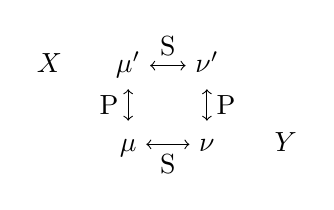
\begin{tikzpicture}

\snode{X}{-1,0}{X};

\snode{MUP}{0,0}{\mu'};
\snode{MU}{0,-1}{\mu};

\snode{NUP}{1,0}{\nu'};
\snode{NU}{1,-1}{\nu};

\snode{Y}{2,-1}{Y};

\draw[<->] (MUP) -- (MU) node [midway, left] () {P};
\draw[<->] (NUP) -- (NU) node [midway, right] () {P};
\draw[<->] (MU) -- (NU) node [midway, below] () {S};
\draw[<->] (MUP) -- (NUP) node [midway, above] () {S};

\end{tikzpicture}
\end{center}
\noindent which suggests that the AO-DF-SOS-MP2 has an overall asymptotic scaling of $\ccpx{3}$. With local density fitting, the graph can however become fully connected
\begin{center}
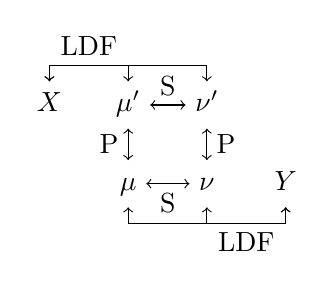
\begin{tikzpicture}

\snode{X}{-1,0}{X};

\snode{MUP}{0,0}{\mu'};
\snode{MU}{0,-1}{\mu};

\snode{NUP}{1,0}{\nu'};
\snode{NU}{1,-1}{\nu};

\snode{Y}{2,-1}{Y};

\draw[<->] (MUP) -- (MU) node [midway, left] () {P};
\draw[<->] (NUP) -- (NU) node [midway, right] () {P};
\draw[<->] (MU) -- (NU) node [midway, below] () {S};
\draw[<->] (MUP) -- (NUP) node [midway, above] () {S};

\draw[<->] (X.north) |- (-0.5,0.5) node[above] {LDF} -| (MUP.north);
\draw[<->] (X.north) |- (-0.5,0.5) node[above] {} -| (NUP.north);

\draw[<->] (Y.south) |- (1.5,-1.5) node[below] {LDF} -| (MU.south);
\draw[<->] (Y.south) |- (1.5,-1.5) node[below] {} -| (NU.south);

\end{tikzpicture}
\end{center}

\noindent where "LDF" is the sparsity relationship introduced between the auxiliary density $X$ and the product density $\cbra{\mu\nu}$, which is metric-specific. In the case of quasi-robust density fitting, LDF = S, and the intermediates $\mathbf{Z}\pa$ can be constructed with linear effort. For weaker decay behaviour, such as the error function coulomb-attenuated metric, the scaling is intermediate between linear and quadratic (Gla2020). 

% Mau2014 https://aip.scitation.org/doi/full/10.1063/1.4881144
% Gla2020 https://pubs.acs.org/doi/abs/10.1021/acs.jctc.0c00600

% QQR screeening:
% S. A. Maurer, D. S. Lambrecht, D. Flaig, and C. Ochsenfeld, J. Chem. Phys. 136, 144107 (2012). https://doi.org/10.1063/1.3693908
%  S. A. Maurer, D. S. Lambrecht, J. Kussmann, and C. Ochsenfeld, J. Chem. Phys. 138, 014101 (2013). https://doi.org/10.1063/1.4770502

\subsection{Local Molecular Orbital MP2}

Problems with PAO based methods: %NJ Russ, TD Crawford J. Chem. Phys., 2004, 121, 691

While linear scaling MP2 was first achived using an atomic orbital formulation, the first low-scaling MP2 implementations were actually formulated in a local molecular orbital basis with domain-specific virtual orbitals (Pul1983-Sae1987). SEPA, electron pairs etc, NESBETS theorem ....

% Pul1983 https://www.sciencedirect.com/science/article/pii/0009261483807039?via%3Dihub
% Sae1985 https://www.sciencedirect.com/science/article/pii/000926148585003X
% Pul1986 https://link.springer.com/article/10.1007/BF00526697 (ORBITAL INVARIANT)
% Sae1987 https://aip.scitation.org/doi/abs/10.1063/1.452293
% Sae1988 https://aip.scitation.org/doi/abs/10.1063/1.454111

\subsubsection{Laplace LMP2}

In the local molecular orbital basis, the Fock matrix is no longer diagonal, and the amplitudes $t_{ia}^{jb}$ can no longer be easily expressed in a local basis, due to the energy denominator. AO-MP2 tackle this problem by virtue of the Laplace transform. Similarly, one can obtain an energy expression in the LMO basis. The Laplace decomposed MP2 energy is given by
\begin{equation}
E_{MP2} = \sum_{\alpha}^{n} \sum_{iajb} |w\pa| e^{(\eps_i + \eps_j - \eps_a - \eps_j)t\pa} \left[2\cn{ia}{jb} - \cn{ib}{ja}\right] \cn{ia}{jb}  
\end{equation}
\noindent Introducing the unitary occupied and virtual LMO-MO transformation matrix $\mathbf{U}$ 
\begin{equation}
\ket{i} = U_{i\uli} \ket{\uli}
\end{equation} 
\begin{equation}
\ket{a} = U_{i\ola} \ket{\ola}
\end{equation}
\noindent which is factorized out, Equation ... becomes
\begin{equation}
\begin{split}
E_{MP2} &= \sum_{\alpha}^{n} \sum_{iajb} \sum_{\uli\ola\olb} \sum_{\ulk\olc\ull\old} |w\pa| e^{(\eps_i + \eps_j - \eps_a - \eps_j)t\pa} U_{i\uli} U_{a\ola} \left[2\cn{\uli\ola}{\ulj\olb} - \cn{\ulj\olb}{\ulj\olb}\right] U_{j\ulj} U_{b\olb} \\
& \qquad \qquad U_{i\ulk} U_{a\olc} \cn{\ulk\olc}{\ull\old} U_{j\ull} U_{b\old} \\  
&= \sum_{\alpha}^{n} \sum_{\uli\ola\olb} \left[2\cn{\uli\ola}{\ulj\olb} - \cn{\ulj\olb}{\ulj\olb}\right] \sum_{\ulk\olc\ull\old} X_{\uli\ulk}\pa Y_{\ola\olc}\pa \cn{\ulk\olc}{\ull\old} X_{\ulj\ull}\pa Y_{\olb\old}\pa \\
&= \sum_{\uli\ola\olb} \left[2\cn{\uli\ola}{\ulj\olb} - \cn{\ulj\olb}{\ulj\olb}\right] \mathcal{T}_{\uli\ola\ulj\olb}
\end{split}
\end{equation}
\noindent with the Laplace amplitudes $\mathcal{T}$ and the Laplace matrices
\begin{equation}
X_{\uli\ulk}\pa = \sum_i U_{i\uli} |w\pa|^{1/4} e^{\eps_i t\pa} U_{k\ulk}
\end{equation}
\begin{equation}
Y_{\ola\olc}\pa = \sum_a U_{a\ola} |w\pa|^{1/4} e^{-\eps_a t\pa} U_{c\olc}
\end{equation}
\noindent Equation ... is the general expression for the MP2 energy in a local molecular orbital basis, where both the occupied and virtual orbitals are \emph{orthogonal}. The situation changes slightly when using non-orthogonal PAOs, as PAOs and CMOs are no longer related by a unitary transformation:
\begin{equation}
\ket{I} = P_{Ii} \ket{i}
\end{equation} 
\begin{equation}
\ket{i} = P_{Ii} S_{IJ}^{-1} \ket{J} 
\end{equation}
\noindent with $\mathbf{S}$ being the overlap matrix in the PAO basis. Due to the non-orthogonality of the PAOs, entries in the overlap matrix can become very small which might lead to numerical instability when computing its inverse. For this reason, the inverse $\mathbf{S}^{-1}$ is substituted by a more general \emph{pseudo-inverse} $\mathbf{V}$ with the property (see ...)
\begin{equation}
\mathbf{SVS} = V
\end{equation}
\noindent The Laplace matrices will then take the following form instead (Kat2008)
\begin{equation}
\mathbf{X}\pa = \mathbf{V} \mathbf{A}\pa \mathbf{V} \pdg 
\end{equation}
\begin{equation}
\mathbf{Y}\pa = \mathbf{V} \mathbf{B}\pa \mathbf{V} \pdg 
\end{equation}
\begin{equation}
A_{IK}\pa = \sum_i P_{Ii} |w\pa|^{1/4} e^{\eps_i t\pa} P_{kK}
\end{equation}
\begin{equation}
B_{AB}\pa = \sum_a Q_{Aa} |w\pa|^{1/4} e^{-\eps_a t\pa} Q_{Aa}
\end{equation}
\noindent In practice, only the virtual orbital space is transformed to PAOs, while the occupied space is kept in an orthogonal local orbital representation.


% Kat2008 https://pubs.rsc.org/en/content/articlepdf/2008/cp/b802993h

NESBETS THEOREM

\subsubsection{Orbital Invariant MP2}

Alternatively, the local MP2 amplitudes can be determined iteratively via an \emph{orbital-invariant} formulation of the MP2 energy expression. Orbital-invariant MP2 predates LT-MP2 by a decade and is based on the \emph{Hylleraas functional} (Hyl,Pul1986). The  Hylleraas functional form of the energy is given by minimizing 
\begin{equation}
E^{(2)} = min \left[ 2\bra{\Psi^{(1)}} \mathbf{H} - E_0  \ket{Psi^{(0}} - \bra{\Psi^{(1)}} \mathbf{H}_0 - E_0 \ket{\Psi^{(1)}} \right]
\end{equation}
\noindent In the case of MP2, the qunatities in Equation ... take the form
\begin{equation}
\bra{\Psi^{(1)}} \mathbf{H} - E_0  \ket{\Psi^{(0}} = \frac{1}{4} \sum_{ijab} t_{ijab} \bra{ij}\ket{ab}
\end{equation}
\begin{equation}
\bra{\Psi^{(1)}} \mathbf{H}_0 - E_0 \ket{\Psi^{(1)}} = \frac{1}{8} \sum_{ijabc} t_{iajb} f_{cb} t_{iajc} - \frac{1}{8} \sum_{ijkab} t_{iajb} f_{jk} t_{iakb}
\end{equation}
\noindent Minimization of the MP2 Hylleraas functional, with respect to the amplitudes $\mathbf{t}$ yields a set of linear equations given by
\begin{equation}
\begin{split}
R_{iajb} = \bra{ij} {} \ket{ab} + \sum_c \left(t_{ijab} f_{cb} + f_{ac} t_{iacb} \right) - \sum_k \left( t_{iakb} f_{kj} + f_{ik} t_{kajb} \right) = 0
\end{split}
\end{equation}
\noindent where $\mathbf{R}$ is the residual. The amplitudes $\mathbf{t}$ are then no longer computed directly by a closed expresion, but iteratively by solving the system of equations, in a similar vein to coupled cluster. This method is said to be orbital invariant, because any molecular orbital representation can be used. For a set of orthogonal MOs $\uli$ and $\ola$, the quantities in Equation ... are simply replaced by their local equivalent. As was the case in LT-LMP2, if PAOs are to be used for the virtual orbital space, the non-orthogonality needs to be taken into consideration. For a mixed LMO-PAO basis, Equation ... reads
\begin{equation}
\begin{split}
R_{\uli A \ulj B} = & \bra{\uli\ulj}{}\ket{AB} + \sum_C \left( f_{AC} t_{\uli C \ulj L} S_{L B} + S_{AC} t_{\uli C \ulj D} f_{DB} \right) \\
&-  \sum_{\ulk} \left( f_{\uli \ulk} S_{AC} t_{\ulk C \ulj D} S_{D B} + f_{\ulk \ulj} S_{AC} t_{\uli C \ulj D} S_{DB} \right) = 0
\end{split} 
\end{equation}
\noindent For specific virtual orbitals, the equations are solved individually for each electron pair $ij$ to obtain their amplitude $\mathbf{t}_{ij}$ and then compute the pair correlation energy. 

why not AO?

\subsubsection{Quadratic Scaling LMP2}

Similar to CEPA, the MP2 energy can be computed as a sum of electron pair energies
\begin{equation}
E_{MP2} = \sum_ij e_{ij}
\end{equation}
\begin{equation}
e_{ij} = \left( 2t_{ij}^{ab} - t_{ij}^{ba} \right) \cn{ia}{jb} 
\end{equation}
\noindent where the amplitudes $t_{ijab}$ are computed according to Eq. ... . The occupied molecular orbitals $ij$ are localized using e.g. Foster-Boys, Pipiek-Mezey or a Cholesky decomposition of the density matrix. Virtual orbitals are generally localized by projection onto the atomic orbital space (PAOs) and subsequently assigning them to pair domains $[ij]$ (domain specific virtuals), or by diagonalizing the MP2 density matrix for each electron pair (pair natural orbitals).  In all cases, the number of SVOs scales as $\mathbf{O}(1)$ for each electron pair $ij$, in the limit of large molecules (see ...). 
 
For well localized orbitals, the electron pair correlation $e_{ij}$ decays with $1/r_{ij}^6$ whith the distance between orbital centres. Electron pairs are generally divided into four groups: strong pairs ($r_{ij} < 1a_0$), weak pairs ($1 < r_{ij} \leq 8 a_0$), distant pairs ($8 < r_{ij} \leq 15 a_0$), and very distant pairs ($15 < r_{ij}$) (Sch1999). Other than by distance criteria, electron pairs can also be grouped by their pair energy (Nee2009). Figure ... shoes the number of significant electron pairs in each category for glycine chains. The number of strong, weak and distant pairs scale as $\mathcal{O}(N)$, while the number of very distant pairs scales quadratically. 

The major bottle-neck in LMP2 is, as usual, the transformation of the 2 electron integrals from the AO basis into the local basis
\begin{equation}
\cn{\uli\ola}{\ulj\olb} = L_{\mu \uli} L_{\sigma \ola} \cn{\mu\sigma}{\nu\lambda} L_{\nu \ulj} L_{\lambda \olb}
\end{equation}
\noindent The expression above translates into the sparsity diagram
\begin{center}
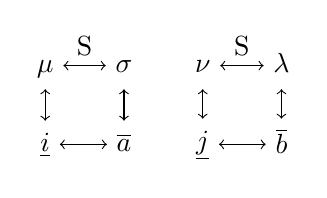
\begin{tikzpicture}

\snode{MU}{0,0}{\mu};
\snode{SIG}{1,0}{\sigma};
\snode{NU}{2,0}{\nu};
\snode{LAM}{3,0}{\lambda};

\snode{I}{0,-1}{\uli};
\snode{A}{1,-1}{\ola};
\snode{J}{2,-1}{\ulj};
\snode{B}{3,-1}{\olb};

\draw[<->] (MU) -- (SIG) node [midway, above] () {S};
\draw[<->] (NU) -- (LAM) node [midway, above] () {S};
\draw[<->] (I) -- (MU) node [midway, below] () {};
\draw[<->] (A) -- (SIG) node [midway, below] () {};
\draw[<->] (J) -- (NU) node [midway, below] () {};
\draw[<->] (B) -- (LAM) node [midway, below] () {};
\draw[<->] (I) -- (A) node [midway, below] () {};
\draw[<->] (J) -- (B) node [midway, below] () {};

\end{tikzpicture}
\end{center}
\noindent which indicates that the MO integrals can be evaluated with $\ccpx{2}$ effort without further approximations. One thing to note is that the quadratic scaling is also obatined, even if the sparsity relationships $i \leftrightarrow a$ and $j \leftrightarrow b$ did not exist, i.e. where virtual orbitals are localized, but not grouped into (apir) domains. The major disadavantage of such non-pair specific methods is that the virtual orbital space is less compact, which leads to a high overhead for integral transformation involving virtual orbitals, which could be the reason that there are no examples in literature using such a scheme. Establishing an a priori sparsity relationship between occupied and virtual space allows to more easily reach the low-scaling regime. 

\begin{figure}
\centering
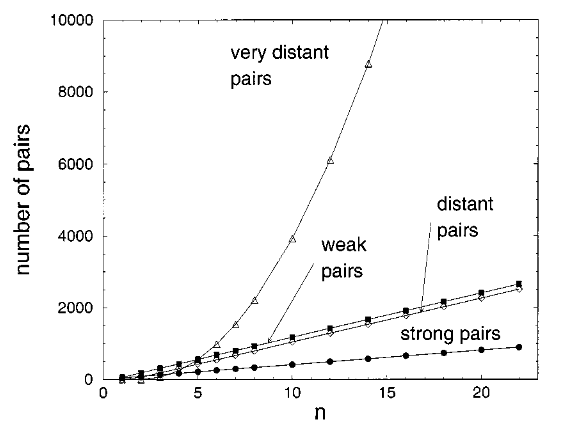
\includegraphics[scale=0.5]{Pics/electron_pairs.png}
\caption{Taken from Sch1999}
\end{figure}

\subsubsection{Linear Scaling LMP2}

It has been found [Sae1987] early on that the quadratic scaling very distant electron pairs can safely ignored without major impact on the total correlation energy. (Distance or Connectivity ciriteria) Distant pairs can also be approximated either by a multipole expansion (Het1998) or empirically (Rau1995), which further lowers the prefactor of the method. As a consequence, this establishes a sparsity relationship between $i$ and $j$, and the sparsity diagram for the MO integrals becomes fully connected
\begin{center}
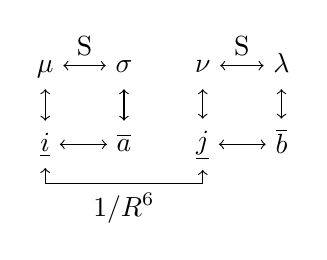
\begin{tikzpicture}

\snode{MU}{0,0}{\mu};
\snode{SIG}{1,0}{\sigma};
\snode{NU}{2,0}{\nu};
\snode{LAM}{3,0}{\lambda};

\snode{I}{0,-1}{\uli};
\snode{A}{1,-1}{\ola};
\snode{J}{2,-1}{\ulj};
\snode{B}{3,-1}{\olb};

\draw[<->] (MU) -- (SIG) node [midway, above] () {S};
\draw[<->] (NU) -- (LAM) node [midway, above] () {S};
\draw[<->] (I) -- (MU) node [midway, below] () {};
\draw[<->] (A) -- (SIG) node [midway, below] () {};
\draw[<->] (J) -- (NU) node [midway, below] () {};
\draw[<->] (B) -- (LAM) node [midway, below] () {};
\draw[<->] (I) -- (A) node [midway, below] () {};
\draw[<->] (J) -- (B) node [midway, below] () {};
\draw[<->] (I) |- (1,-1.5) node [below] {$1/R^6$} -| (J);

\end{tikzpicture}
\end{center}
\noindent and linear scaling LMP2 therefore becomes possible (Sch1999).

% Sch1999 https://aip.scitation.org/doi/pdf/10.1063/1.479957

% distant pairs multipole approximate very distant pairs by multipole expansion Het1998 https://www.sciencedirect.com/science/article/pii/S0009261498004916

% distant pairs Empirically Rau1995 G. Rauhut, J. W. Boughton, and P. Pulay, J. Chem. Phys., 103, 5662 1995 .

Instead of using distance criteria, can use screening: 
%https://aip.scitation.org/doi/10.1063/1.4773581

\subsubsection{Density Fitting for LMP2}

While specific virtual orbitals form a very compact representation of the virtual space, the fact that each electron pair has their own orthogonal vitual orbital basis means that the total number of virtuals can become exceedingly large, and consequently increases the cost associated with the AO-MO transformation step. The most expensive step then becomes
\begin{equation}
\cn{\uli\ola}{P} = L_{\mu\uli} \cn{\mu\nu}{P} L_{\nu\ola}
\end{equation}
\noindent Transformation of the 3c2e integrals scales with $\ccpx{2}$. Linear scaling can be achieved by instroducing an orbital-specific fitting domain $[i]_fit$, e.g. by assigning all auxiliary functions $P$ on atoms with a Mulliken charge above a given threshold for the local orbital $i$ (Pin2015), or by using a Boughton-Pulay like scheme (Wer2015). This yields the sparsity diagramm
\begin{center}
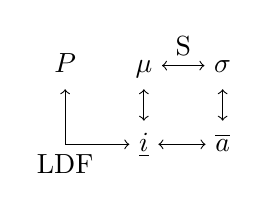
\begin{tikzpicture}

\snode{P}{-1,0}{P};
\snode{MU}{0,0}{\mu};
\snode{SIG}{1,0}{\sigma};

\snode{I}{0,-1}{\uli};
\snode{A}{1,-1}{\ola};

\draw[<->] (MU) -- (SIG) node [midway, above] () {S};
\draw[<->] (I) -- (MU) node [midway, below] () {};
\draw[<->] (A) -- (SIG) node [midway, below] () {};
\draw[<->] (I) -- (A) node [midway, below] () {};
\draw[<->] (I) -- (-1,-1) node [below] {LDF} -- (P);

\end{tikzpicture}
\end{center}
\noindent As opposed to SOS-AO-MP2, where density fitting can give a more favourable factorization of the energy expression, the MO integrals need to fully assembled for LMP2 in order to solve the linear equations (...). The assembly is done in two steps
\begin{equation}
B^{X}_{\uli\ola} = \sum_{Y \in [i]_{fit} \cup [j]_{fit}} \cn{X}{Y}^{-1/2} \cn{Y}{\uli\ola}
\end{equation}
\begin{equation}
\cn{\uli\ola}{\ulj\olb} = \sum_{X \in [i]_{fit} \cup [j]_{fit}} B^{X}_{\uli\ola} B^{X}_{\ulj\olb} 
\end{equation}
\noindent The two steps are repeated for each electron pair $ij$, and the sum runs over all auxiliary functions $P$ in the unified fitting domain $[i]_{fit} \cup [j]_{fit}$, which enforces linear scaling for these steps as well. 

% Pin2015 https://aip.scitation.org/doi/pdf/10.1063/1.4926879
% Wer2015 https://pubs.acs.org/doi/pdf/10.1021/ct500725e

\subsection{Atomic Orbital Coupled Cluster}

\subsection{Local Coupled Cluster}

\subsection{FNO Coupled Cluster ??}

% Hylleraas functional: 
% Hyl1930 https://link.springer.com/article/10.1007/BF01397032

% First use of LMO+PNOs with Hylleraas 
% Pul1986 https://link.springer.com/article/10.1007%2FBF00526697

% LInear scaling of the functional
% Linear scaling of electron inetgrals
% linear scaling of MO-AO transformation -> or density fitting



\chapter{Local Correlation Methods (III): Excited States}

While local correlation methods for the ground state have been around since the 1980s, the extension of the local treatment of electron correlation to excited states is relatively new. With the earliest attempts dating back to the 2000s, many new approaches and approximations have emerged over the last decade, building on the concepts of LMOs, NOs and PNOs. One of the major obstacles that makes a straight-forward extension to excited states difficult is the long-range character of certain excitations, such as charge transfer states. In contrast to the description of electron correlation in the ground state, the occupied and virtual orbitals involved in electron transitions can be very far apart. This means that the optimal molecular orbital space for the excited state can be very different from that of the ground state. 

This chapter presents the state of the art for local correlated excited state methods (ADC, CCLR, EOM-CC) for LMOs, NOs, PNOs, and combinations thereof. Atomic orbital approaches are discussed as well. 

% Bau2017 CornFlex https://aip.scitation.org/doi/pdf/10.1063/1.4984820

% Linear‐scaling self‐consistent field methods for large molecules
% https://aip.scitation.org/doi/pdf/10.1063/1.2961039

\section{Low-Scaling Correlated Excited State Methods}

All of the existing low-scaling implementations of ADC, CCLR and EOM use some form of local or compact molecular orbital representation, to varying degrees of success. As mentioned above, the major problem that these methods face is the non-locality of certain excited states such as charge transfer states, which can involve occupied and virtual orbitals which are localized on entirely different parts in the system. Clearly, truncating virtual orbitals spatially is no longer a valid option, and makes a straight-forward extension of LMO-methods difficult, because they cut out far-away contributions. Similar problems are encountered in NO formulations, as the excited state is often not properly described by the electronic ground state (pair-)densities and their associated (pair) natural representation. Over the years, various strategies have been proposed to adapt existing LMO and NO schemes to excited states as well. 

\subsection{Orbital Invariance of the Matrix Expressions}

Correlated excited state methods involve some form of symmetric or non-symmetric eigenvalue problem, which is generally solved using the Davidson procedure. The time-determining step is given by the computation of the matrix-vector product of the ADC, CC response, or EOM-CC matrix $\mbf{A}$ with the Davidson trial vectors $\mbf{u}$
\begin{equation}
\mbf{r} = \mbf{A} \mbf{u}
\end{equation}
\noindent Closed expressions can be derived for the MVPs, with the matrix elements computed on the fly. The MVPs and trial vectors are divided into blocks of singles, doubles, triples, ... ($u_i^a$, $u_{ij}^{ab}$, $u_{ijk}^{abc}$) depending on the level of approximation of the underlying methods. In the case of ADC(2), the MVP is split according to
\begin{align}
r_{ia} &= A_{ia,jb} u_{jb} + A_{ia,jbkc} u_{jbkc} \\
r_{iajb} &= A_{iajb,kc} u_{kc} + A_{iajb,kcld} u_{kcld} 
\end{align}
\noindent The eigenvalue problem is generally solved in the canonical molecular orbital basis, but other orbital representations can also be used, by swapping all the CMO quantities $\cn{ia}{jb}$, $t_{iajb}$, ... by their local counterparts $\cn{\uli\ola}{\ulj\olb}$, $t_{\uli\ola\ulj\olb}, ...$. The eigenvalue problem can then be solved e.g. in an LMO basis, or the MVPs can be computed in the LMO basis and transformed to the CMO basis using the transformation matrix $\mbf{U}$:
\begin{equation}
r_{ia} = U_{i\uli} r_{\uli\ola} U_{\ola a} 
\end{equation}
\noindent The eigenvalues of the LMO matrix appear to not differ from the ones obtained via a CMO formalism \cite{Kat2009}.

For local EOM-CC and CCLR, the singles and doubles amplitudes $t_{\mu_1}$ and $t_{\mu_2}$ are determined iteratively from a local ground state calculations using the techniques in the previous chapter for reduced scaling. For the approximate EOM-CC2 and CC2-LR methods, as well as ADC(2), the MP2 amplitudes may also be computed iteratively in the local basis using the Hylleraas functional, or using a closed form expression via the Laplace transform techniques.   

EOM-CC2, CC2-LR and ADC(2) allow for an on-the-fly computation of the doubles part (see section \ref{sec:ADC_DAV}). Here, the orbital invariant formulation becomes less straight-forward because the doubles-doubles block of the non-canonical ADC and CC2 Jacobian matrix is not diagonal. Fortunately, the Laplace transform can be applied to circumvent this problem. Using the ADC(2) eigenvalue problem as an example, the doubles-folded MVP expression is given by
\begin{equation}
\begin{split}
r_{ia}(\omega) &= A_{ia,jb} u_{jb} + A_{ia,jbkc} \frac{A_{iajb,kc} u_{kc}}{\omega - \eps_a - \eps_b + \eps_i + \eps_j} \\
&= A_{ia,jb} u_{jb} - \sum_{\alpha}^{n} |w\pa| e^{\left(\omega - \eps_a - \eps_b + \eps_i + \eps_j\right) t\pa} A_{ia,jbkc} A_{,kc} u_{kc} 
\end{split}
\end{equation}
After transforming to the LMO basis, the local ADC(2) equations read
\begin{equation}
r_{\uli \ola}(\omega) = A_{\uli \ola, \ulj \olb} u_{\ulj \olb} - A_{\uli \ola, \ulj \olb \ulk \olc} \sum_{\alpha}^{n} e^{\omega t\pa} X_{\ulj \ulj'}\pa Y_{\olb \olb'}\pa A_{\ulj' \olb' \ulk' \olc', \ull \old} u_{\ull \old} X_{\ulk \ulk'}\pa Y_{\olc \olc'}\pa  \\
\end{equation}
\noindent with the Laplace matrices $\mathbf{X}$ and $\mathbf{Y}$ 
\begin{equation}
X_{\uli\ulk}\pa = \sum_i U_{i\uli} |w^{'(\alpha)}|^{1/4} e^{\eps_i t^{'(\alpha)}} U_{k\ulk}
\end{equation}
\begin{equation}
Y_{\ola\olc}\pa = \sum_a U_{a\ola} |w^{'(\alpha)}|^{1/4} e^{-\eps_a t^{'(\alpha)}} U_{c\olc}
\end{equation}
\noindent Note that the optimal Laplace parameters $w^{'(\alpha)}$ and $t^{'(\alpha)}$ are different from the ones used in the MP2 amplitudes, due to the presence of the eigenvalue $\omega$ in the denominator. Each time the eigenvalue changes, the Laplace parameters need to be recomputed to obtain an accurate approximation. 

An orbital invariant reformulation is not needed by every method. NOs, PNOs and NTOs can be \emph{canonicalized} by diagonalizing the occupied-occupied and virtual-virtual block of the Fock matrix in the truncated NO/PNO/NTO basis to get a smaller set of canonical molecular orbitals and orbital energies. Because these types of representations generally do not depend on distance criteria, they are unaffected by the delocalized nature of the canonical basis, as they seek compactness rather than locality. 

\subsection{Local Molecular Orbitals and Domains}

The most challenging part in extending domain-specific virtual orbital methods to excited states lies in determining a suitable excitation domain in which to expand the virtual space. The first implementations of local excited state EOM-CCSD \cite{Cra2002,Kor2003} and CC2-LR \cite{Kat2006} constructed the domains using a Mulliken-charge like analysis of the CIS coefficients $r_{ia}$. The CIS coefficients are first transformed to the LMO-PAO basis
\begin{equation}
r_{\uli \olgm} = U_{\uli i } r_{ia} \bar{C}_{\mu a} 
\end{equation}
\noindent To determine the importance $w$ of each LMO/PAO, the squares of the norms of the coefficients are summed up row- and column-wise
\begin{equation}
\begin{split}
w_{\uli} &= \sum_{\mu} |r_{\uli \olgm}|^2 \\
w_{\olgm} &= \sum_{\uli} |r_{\uli \olgm}|^2
\end{split}
\end{equation}
\noindent The LMOs/PAOs are then ordered by decreasing weight. Their weights are then summed up until a certain threshold $T_{LMO}$/$T_{PAO}$ is reached (typically around 0.995 to 0.9999). The excited state orbital domains $[\uli]_{ES}$ containing the relevant virtual orbitals are then constructed by applying the Boughton-Pulay algorithm to a set of "excited natural orbitals" \cite{Kor2003}
\begin{equation}
\phi_{\uli}^* = \sum_{\ola} r_{\uli \olgm} \phi_{\olgm}  
\end{equation} 
\noindent The full orbital domain of $i$ is then given as the union of its ground-state and excited state domain $[\uli]$ = $[i]_{GS} \cup [i]_{ES}$. The virtual orbital weights $w_{\olgm}$ can be used to impose further restrictions on the virtual orbital space. Finally, the pair domains $ij$ are formed as the union $[\uli] \cup [\ulj]$. In general, only the computation of the doubles part, which is time-determining, is subject to domain-restrictions, while the singles part is computed without domain lists.

The method however has the major flaw that the orbital domains are highly sensitive to the CIS transition density, which does not describe the excited state very accurately. Some orbitals can be dropped in the domain construction which might become important for doubles contributions. LMO methods face an interesting chicken-or-egg problem where they need information from the excited state wave function, to accurately compute properties of said function. There are several ways to address this problem. In their local CC2-LR implementation, Kats and Schütz \cite{Kat2009} use Laplace transformed doubles folding to recompute the doubles amplitudes on the fly, which allows to adapt the excited state domains dynamically during the optimization procedure. Starting from the CIS transition density, the domains are recomputed at each step by analyzing the state vector $r_{\uli \olgm}(\omega)$ as described above. This greatly increased accuracy compared to canonical calculations with energy differences well below 0.1 eV.

Mester et al. \cite{Mes2017} proposed a more pragmatic approach, where they first analyze the CIS state vector to extract the important LMOs and PAOs. They then augment the domains $[i]_{EX}$ by adding all remaining molecular orbitals that have a significant Mulliken charge on an atom that is also significant for $i$. This is based on the assumption that, although CIS might not be a good approximation, the important orbitals should still be close by. 

Nonetheless, the LMO method is again plagued by spurious distance dependent thresholds and Mulliken charge thresholds. Nowadays, low scaling excited state methods are mostly dominated by PNOs, NOs, or NTOs.

% Kor2003 First EOM-CCSD Korona, T.; Werner, H.-J. Local treatment of electronexcitations in the EOM-CCSD method.J. Chem. Phys.2003,118,3006.
% Also first EOM-CCSD Cra2002 Crawford, T. D.; King, R. A. Locally correlated equation-of-motion coupled cluster theory for the excited states of largemolecules.Chem. Phys. Lett.2002,366, 611.
% https://aip.scitation.org/doi/10.1063/1.3237134

\subsection{Natural Orbitals}

NO methods achieve performance by dropping virtual natural orbitals with low occupation numbers. The first implementations of EOM-CC and CCLR in the NO representation used natural orbitals obtained from the diagonalization of the ground state MP2 density matrix \cite{Lan2010}. A reasonable speed-up could be observed, although the excited state character was not taken into account. However, it was shown \cite{Kum2017} that properties like the polarizability are much more sensitive to the truncation of the virtual orbitals than the ground state correlation energy, with the error increasing linearly as a function of the number of dropped virtual natural orbitals. While VNOs with low occupation numbers, i.e. diffuse character, can be safely  ignored for the ground state correlation energy, diffuse VNOs play a much more important role for response properties, and hence fewer VNOs can be omitted. Better results could be obtained by simply truncating the virtual CMOs instead, which invalidates the use of VNOs. 

In their NO-CC2 and NO-ADC(2) implementations, Mester et al. \cite{Mes2017, Mes2018, Mes2019} proposed to compute a set of occupied and virtual NOs by diagonalizing the occupied and virtual state-averaged densities
\begin{equation}
\mathbf{D}_{ij} = \frac{1}{2} \left( \mathbf{D}_{ij}^{MP2} + \mathbf{D}_{ij}^{CIS(D)} \right)
\end{equation}
\begin{equation}
\mathbf{D}_{ab} = \frac{1}{2} \left( \mathbf{D}_{ab}^{MP2} + \mathbf{D}_{ab}^{CIS(D)} \right)
\end{equation}
\noindent where $\mathbf{D}^{MP2}$ is the MP2 ground state density and $\mathbf{D}^{CIS(D)}$ is the state-specific CIS(D) excited state density. Their restricted expressions read
\begin{equation}
D_{ij}^{MP2} = \sum_{kab} \left( 2 t_{ik}^{ab} t_{jk}^{ab} - t_{ik}^{ab} t_{jk}^{ab} \right) 
\end{equation}
\begin{equation}
D_{ab}^{MP2} = \sum_{ijc} \left( 2t_{ij}^{ca} t_{ij}^{cb} - t_{ij}^{ca}t_{ij}^{bc} \right)
\end{equation}
\begin{equation}
D_{ij}^{CIS(D)} = \sum_{a} c_i^a c_j^a  + \sum_{kab} \left( 2 t_{ik}^{ab} t_{jk}^{ab} - t_{ik}^{ab} t_{jk}^{ab} \right) 
\end{equation}
\begin{equation}
D_{ab}^{CIS(D)} = \sum_{i} c_i^a c_i^b + \sum_{ijc} \left( 2c_{ij}^{ca} c_{ij}^{cb} - c_{ij}^{ca}c_{ij}^{bc} \right)
\end{equation}
\noindent where $c_i^a$ are the CIS coefficients and the $c_{ij}^{ab}$ are the CIS(D) doubles coefficients
\begin{equation}
c_{ij}^{ab} = \frac{\sum_c \left[ \cn{ac}{bj} c_i^c + \cn{ac}{bi} c_j^c \right] - \sum_k \left[ \cn{kj}{ai} c_k^b + \cn{kj}{bj} c_k^a \right]}{D_{ij}^{ab} + \omega_{CIS}}
\end{equation}
\noindent The state-averaged density needs to be recomputed and diagonalized for each state because $\mathbf{D}^{CIS(D)}$ depends on the excitation energy $\omega$. While the CIS(D) density is much easier to compute than the ADC(2) or CC2-LR state density, it still scales with $\ccpx{5}$. To reduce the computational complexity, the density is constructed in a truncated orbital space: first, a set of occupied and virtual LMOs are chosen according to the CIS weighting criteria $w$ described in the previous section. The basis is augmented by spatially close orbitals, and then canonicalized to yield a highly compact orbital molecular space which lowers the cost of constructing the CIS(D) densities. 

In combination with natural auxiliary functions, this hybrid NO-LMO scheme can reduce the timings for CC2 and ADC(2) to such a drastic extent that the CIS pre-iterations become the time-determining step (Figure \ref{fig:MESTER}), with an additional error of only 2-4 meV. The reduced scaling however comes at a high prefactor when computing multiple different excitation energies. 

\begin{figure}
\centering
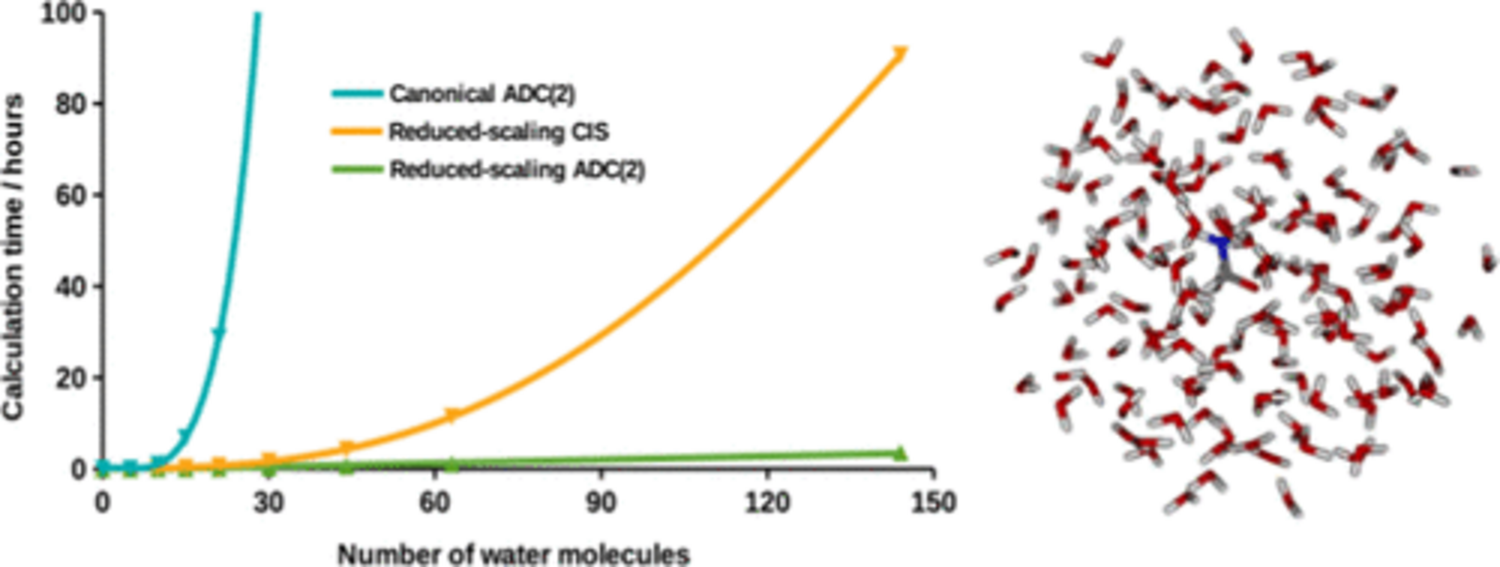
\includegraphics[scale=1.0]{Pics/mester_adc.png}
\caption[Wall times of CIS compared to NO-ADC(2) as a function of system size of hydrated formamide.]{Wall times of CIS compared to NO-ADC(2) as a function of system size of hydrated formamide. Taken from \cite{Mes2019}.}
\label{fig:MESTER}
\end{figure}

% Reduced NO CC2 Mes2017 https://aip.scitation.org/doi/10.1063/1.4983277
% EOM NO Lan2010 https://aip.scitation.org/doi/10.1063/1.3276630
% CCLR NO Kum2017 https://pubs.acs.org/doi/10.1021/acs.jpca.6b11410
% Reduced ADC(2) Mes2018 https://aip.scitation.org/doi/10.1063/1.5021832
% Reduced ADC(2) Mes2019  https://pubs.acs.org/doi/pdf/10.1021/acs.jctc.9b00735
% CIS(D) Hea1994 https://www.sciencedirect.com/science/article/pii/0009261494000700?via%3Dihub

\subsection{Pair Natural Orbitals}

Pair natural orbital methods face the same problems as NOs, where PNOs with low occupation numbers are considerably more important for response properties than for ground state properties \cite{McA2016}. In a similar vein, excited state PNOs can be generated by considering lower level excited state electron pair densities \cite{Hel2011}. PNO methods have been successfully extended to ADC(2), CC2-LR \cite{Hel2013}, ADC(2)-x \cite{Hel2014} and CCSD-LR \cite{Fra2018} by using CIS(D) or CIS(D)-like densities
\begin{equation}
D_{ij}^{ab} = \sum_c \left( 2b_{ij}^{ab} - b_{ij}^{ba} \right) b_{ij}^{ab} + \left( 2b_{ij}^{ab} - b_{ij}^{ba} \right) b_{ij}^{ba}
\end{equation}
\noindent where $\mathbf{b}_{ij}$ are state-specific modified pair amplitudes which are not uniquely defined. Again, these methods come at the cost of a higher prefactor due to the relatively high cost of constructing PNOs. %Nonetheless, it was shown that the computational complexity can be lowered to $\ccpx{3}$ for PNO-CCSD-LR. 

Efforts have also been made to develop PNO response methods which are more economical for computing larger excitation manifolds by removing the state-specificity. Instead of taking individual excited state densities, Peng et al. \cite{Pen2018} proposed to generate a set of \emph{state-averaged} PNOs obtained by diagonalization of the average excited state density over an $N$-state manifold 
\begin{equation}
\mathbf{D}_{ij} = \frac{1}{N} \sum_k^N \mathbf{D}_{ij}^{(k)}
\end{equation}
\noindent A production-quality implementation has not yet been shown which uses this approach.

In their perturbed pair-natural orbital (PNO++) approach for CCLR, Cunha and Crawford \cite{DCu2021} incorporate the external perturbation into the electron pair density
\begin{equation}
D_{ij}^{ab} = \sum_c \left( 2x_{ij}^{ab} - x_{ij}^{ba} \right) x_{ij}^{ab} + \left( 2x_{ij}^{ab} - x_{ij}^{ba} \right) x_{ij}^{ba}
\end{equation}
\noindent where $\mathbf{x}$ are perturbed amplitudes given by
\begin{equation}
x_{ij}^{ab} = \frac{\overline{B}}{\ovl{H}_{aa} + \ovl{H}_{bb} - \ovl{H}_{ii} - \ovl{H}_{jj} + \omega}
\end{equation}
\noindent with an external perturbation $\ovl{B}$ and the similarity transformed Hamiltonian $\ovl{H}$. This gives a set of "perturbation-aware" PNOs customized for a given external perturbation \cite{Cra2019}. 

Finally, there are also the \emph{back-transformed} PNOs, or bt-PNOs, where the ground state PNO-quantities like the amplitudes are transformed back to the canonical basis and used in the canonical working equations \cite{Dut2016}.

In the end, most local excited state methods using natural orbitals differ by how they redefine the amplitudes $\mathbf{b}$ for the individual excited states or the whole perturbed molecular system. It is still an active field of research.

% PNO-CIS(D) Hel2011 https://aip.scitation.org/doi/10.1063/1.3664902 [Uses CIS(D) pair density]
% PNO-CC2 Hel2013 https://aip.scitation.org/doi/10.1063/1.4819071 [Uses Excited state OSVs to construct PNOs] 
% PNO-ADC(2)-x: Hel2014 https://www.sciencedirect.com/science/article/pii/S2210271X14001194?via%3Dihub [Also use excited state specific desnity to get OSVs using modified CIS(D) like desnities CC2/ADC(2)-x densities Dii_ab
% PNO-CCSD https://aip.scitation.org/doi/full/10.1063/1.5018514 [Also CIS(D) like density] 

% PNOs have similar Problem than NOs: Har2016  https://pubs.acs.org/doi/10.1021/acs.jctc.5b00898
% Because diffuseness. Solution: Cra2019 PNO++ https://onlinelibrary.wiley.com/doi/10.1002/wcms.1406
% PNO++-CCSD-LR Cun2021 https://pubs.acs.org/doi/pdf/10.1021/acs.jctc.0c01086

% State-averaged Pen2018 https://arxiv.org/pdf/1802.06738.pdf
% bt-PNOs Dut2016 https://aip.scitation.org/doi/pdf/10.1063/1.4958734
 
\subsection{Natural Transition Orbitals}

The last method to obtain a compact representation of excited states is via natural transition orbitals. NTOs are the equivalent of NOs for excited states, and represent a compact representations of their dominant contribution (Figure \ref{fig:NTO}). Baudin and Kristensen have developed two different CC2-LR schemes based on NTOs called LoFEX (local framework for calculating excitation energies) \cite{Bau2016} and CornFLEX (correlated natural transition orbital framework for calculating excitation energies) \cite{Bau2017} 

Again, one needs information about the excited state to efficiently compute its properties. The LoFEX method starts with a time-dependent Hartree Fock calculation and generates a set of NTOs by decomposition of the TDHF transition vectors $\mathbf{r}$ by diagonalization
\begin{align}
\mathbf{r} \mathbf{r}^{\dagger} \mathbf{U} &= \lambda_o \mathbf{U} \\
\mathbf{r}^{\dagger} \mathbf{r} \mathbf{V} &= \lambda_v \mathbf{V}
\end{align}
\noindent which is just an alternative way to compute the occupied and virtual NTO transformation matrices $\mathbf{U}$ and $\mathbf{V}$, rather than by singular value decomposition. A set of dominant NTO pairs is then chosen for which their occupation numbers are above a given threshold $\tau_{LoFEX}$. The non-dominant NTOs are not discarded, but rather localized. The idea is to construct a surrounding excitation orbital space (XOS) containing LMOs that are important for correlation effects of the NTOs. A first guess to the XOS is chosen based on distance criteria and Löwdin charges. The CC2-LR eigenvalue problem is then solved in that basis, and new NTOs are computed from the CC2 transition vector and added to the XOS. This procedure is repeated until the excitation energy $\omega$ for that state has converged. While the guess XOS is first formed using distance criteria, the subsequent optimization procedure makes the method much more robust and black-box. Even for relatively small molecules, LoFEX can obtain considerable speed-ups. The main disadvantage is that LoFEX does not give any leverage for very delocalized excitations. 

The improved CornFLEX method constructs a set of CIS(D)-like NTOs (CIS(D')-NTOs) which is obtained from diagonalizing a CIS(D)-like density matrix in the CIS-NTO basis. As opposed to CIS-NTOs, the CIS(D') NTOs also include correlation effects and are a more robust representation that the simple ad-hoc extension of CIS-NTOs using LMOs. Speed-ups can be observed in CornFLEX even for delocalized excitations.

% Bau2016 https://aip.scitation.org/doi/pdf/10.1063/1.4953360
% Bau2017 https://aip.scitation.org/doi/pdf/10.1063/1.4984820

\begin{figure}
\centering
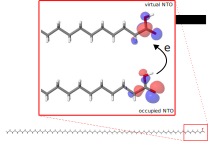
\includegraphics[scale=0.6]{Pics/NTOACID}
\caption[Dominant natural transition orbital pair for the lowest excitation of the carboxylic acid C$_{79}$H$_{159}$COOH.]{Dominant natural transition orbital pair for the lowest excitation of the carboxylic acid C$_{79}$H$_{159}$COOH ($\pi \rightarrow \pi^*$ transition). The span of the NTOs is very small compared to the rest of the molecule, and the compactness can be used to drastically speed up excited state calculations.}
\label{fig:NTO}
\end{figure}

\section{Atomic Orbital Configuration Interaction Singles}

%-> AO TDSCF (Kussmann)
%-> TDHF and RPA are equivalent in linear response regime. % see https://www.frontiersin.org/articles/10.3389/fphy.2019.00020/full

The methods presented in the previous section all work similarly. They first start by approximating the targeted excited states with a lower level of theory using CIS or CIS(D). They then solve higher order equations in the basis obtained from that approximation and may also dynamically augment the correlation domain while optimizing the excitation energies. The methods work on the principle of orbital \emph{compactness} rather than sparsity

At the moment of writing, CIS is the only excited state method which is routinely evaluated using an AO approach. While CIS does not give qualitatively good results, it is still a very important stepping stone for higher order methods, as was demonstrated in the previous section. Omitting the zero-order contributions, the CIS working equations are given by
\begin{equation}
r_{ia} = \left[ 2 \cn{ia}{jb} - \cn{ib}{ja} \right] u_{jb}
\end{equation}
\noindent Factoring out the MO coefficient matrices:
\begin{equation}
\begin{split}
r_{ia} &= C_{\mu i} C_{\sigma a} \left[ 2 \cn{\mu\sigma}{\nu\lambda} - \cn{\mu\lambda}{\nu\sigma} \right] C_{\nu j} C_{\lambda b} u_{jb} \\ 
&= C_{\mu i} C_{\sigma a} \left[ 2 \cn{\mu\sigma}{\nu\lambda} - \cn{\mu\lambda}{\nu\sigma} \right] P_{\nu\lambda} 
\end{split}
\end{equation} 
\noindent where $\mathbf{P}$ is the non-symmetric transition density in the AO basis. The CIS working equations can be reduced to the construction of a "pseudo"-Fock matrix which has a Coulomb and an exchange part. The Fock matrix is then transformed to the MO basis:
\begin{align}
F_{\mu\nu} &= J_{\mu\nu} + K_{\mu\nu}  \\ 
r_{ia} &= C_{\mu i} F_{\mu\nu} C_{\mu a}  
\end{align}
\noindent For localized excitations, the AO transition density is sparse (Figure \ref{fig:CISDENSE}), and similar approximation can be used as in Hartree Fock, e.g. LinK, CFMM, or LDF. CIS can therefore be evaluated with $\mathcal{O}(N)$ computational effort. Strictly speaking, it is not a "pure" AO formulation, because the AO intermediates still need to be transformed to the MO basis.

\begin{figure}
\centering
\begin{subfigure}{0.3\linewidth}
\centering
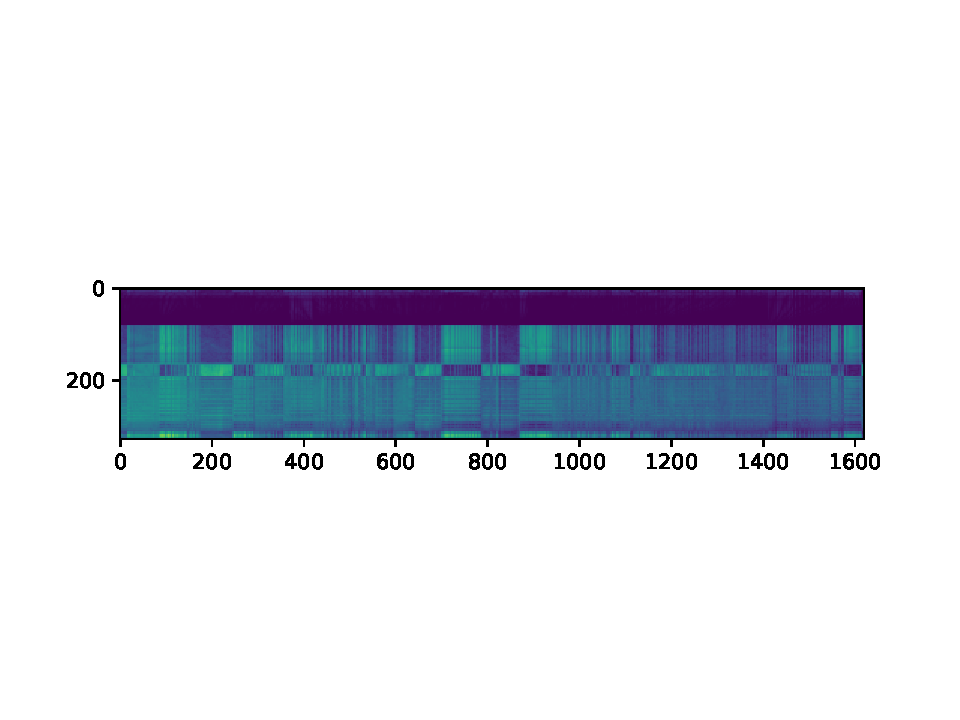
\includegraphics[scale=0.6]{Pics/CISDENSE}
\caption{}
\end{subfigure}
$\Longrightarrow$
\begin{subfigure}{0.6\linewidth}
\centering
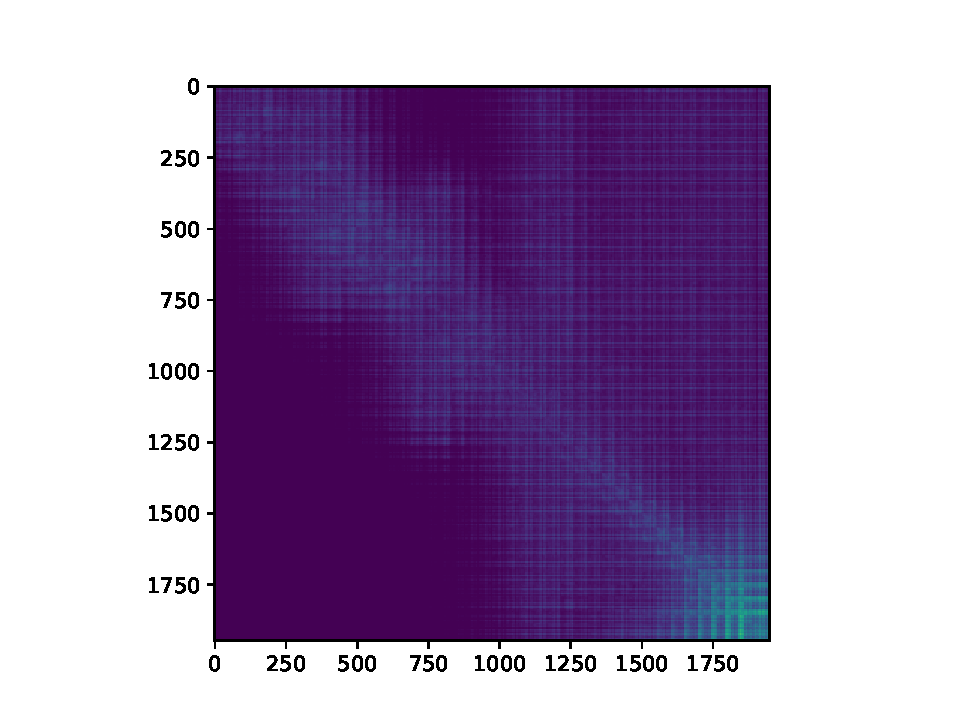
\includegraphics[scale=0.6]{Pics/CIS}
\caption{}
\end{subfigure}
\caption[Logarithm of the absolute values of the matrix elements in the transition densities in the MO and AO basis for the lowest excited state for the carboxylic acid C$_{79}$H$_{159}$COOH.]{Logarithm of the absolute values of the matrix elements in the transition densities in the MO (left) and AO basis (right) for the lowest excited state for the carboxylic acid C$_{79}$H$_{159}$COOH. The excitation domain is entirely localized on the carboxylic group. Using sparse matrix algebra, significant speed-ups can be obtained for CIS in the AO basis.}
\label{fig:CISDENSE}
\end{figure}

% PAO CCLR not good! Look at Gunnar review article perhaps

% First appearance of local EOM-CCSD 
% Cra2002 https://aip.scitation.org/doi/pdf/10.1063/1.1537718

% First appearance of local CCLR CC2 (no doubles wrapping) Kat2006 https://aip.scitation.org/doi/pdf/10.1063/1.2339021
% Flaw: Domains dtermined from CCS, bad if not correponding to good approximat. ALso fixed during davidson

% Kat2009 https://aip.scitation.org/doi/pdf/10.1063/1.3237134
% FIxes Problem by refreshing domains

% state-specific PNOs from CIS(D) Hel2011 https://aip.scitation.org/doi/10.1063/1.3664902

% Hel2013 PNO-CC2 https://aip.scitation.org/doi/10.1063/1.4819071

% Hel2014 PNO-ADC2 https://www.sciencedirect.com/science/article/pii/S2210271X14001194?via%3Dihub

%PURE AO FORMULATION THOULESS INTEGRAL
%PROBLEM: MO ENERGIES ARE NEEDED. if a pure ao algorithm, most likely a whole other approach that tries to get "density metrix perturbation"

\section{Molecular Orbital-free Approaches}

Maybe if I have time
%https://aip.scitation.org/doi/full/10.1063/1.2961039?casa_token=XyapU_j1S9YAAAAA%3A6MKC3CuVoVEGS1bR-G3uHzyMo_UMcvArZKA2EkxO8Pwzc1gJWI0qwUWF6GB1PL7XEjDQH2lwrDniBQ
% https://aip.scitation.org/doi/10.1063/1.2965535

OTHER: \url{https://www.kth.se/blogs/pdc/2018/11/scalability-strong-and-weak-scaling/}

\part{Annex}

- ERI deomposition: cholesky, THC, pseudo-spectral
% cholesky https://link.springer.com/article/10.1007/s00214-009-0608-y
- The evil matrix inversion: considerations
% see https://www.johndcook.com/blog/2010/01/19/dont-invert-that-matrix/ 
% also https://epubs.siam.org/doi/abs/10.1137/1.9780898718027.ch14
- mulliken, boughton pulay

\end{document}